\documentclass[11pt,letterpaper]{article}
\ifdefined\pdfminorversion\pdfminorversion=7\fi
\usepackage[T1]{fontenc}
\usepackage[utf8]{inputenc}
\usepackage{lmodern}
\usepackage[margin=0.88in,headheight=14pt]{geometry}
\usepackage{microtype}
\usepackage{amsmath,amssymb,amsthm,mathtools}
\usepackage{graphicx,booktabs,array,longtable,tabularx}
\usepackage[dvipsnames]{xcolor}
\usepackage{listings}
\usepackage[numbers,sort&compress]{natbib}
\usepackage{enumitem}
\usepackage{fancyhdr}
\usepackage{placeins}
\usepackage{flafter}
\usepackage[colorlinks=true,linkcolor=MidnightBlue,citecolor=MidnightBlue,
  urlcolor=MidnightBlue,breaklinks=true]{hyperref}
\hypersetup{pdftitle={Computing Quantiles of Weighted Bernoulli Sums},
  pdfsubject={Exact algorithms, conservative inequalities, and reproducible R code},
  pdfauthor={}}
\numberwithin{equation}{section}
\newtheorem{theorem}{Theorem}[section]
\newtheorem{proposition}[theorem]{Proposition}
\newtheorem{lemma}[theorem]{Lemma}
\newtheorem{corollary}[theorem]{Corollary}
\theoremstyle{definition}
\newtheorem{definition}[theorem]{Definition}
\theoremstyle{remark}
\newtheorem{remark}[theorem]{Remark}
\newcommand{\E}{\mathbb E}
\newcommand{\Pbb}{\mathbb P}
\DeclareMathOperator{\Var}{Var}
\DeclareMathOperator{\supp}{supp}
\definecolor{CodeBackground}{HTML}{F5F7FA}
\definecolor{CodeBorder}{HTML}{D9E0E8}
\definecolor{CodeComment}{HTML}{516471}
\definecolor{CodeString}{HTML}{8B3D29}
\lstdefinestyle{Rcode}{language=R,
  basicstyle=\ttfamily\fontsize{8.5}{10.4}\selectfont,
  keywordstyle=\color{MidnightBlue},commentstyle=\color{CodeComment},
  stringstyle=\color{CodeString},backgroundcolor=\color{CodeBackground},
  frame=single,rulecolor=\color{CodeBorder},framerule=0.3pt,
  framesep=6pt,aboveskip=10pt,belowskip=10pt,
  showstringspaces=false,upquote=true,keepspaces=true,
  columns=fullflexible,breaklines=true,breakatwhitespace=false,
  tabsize=2,captionpos=b}
\lstdefinestyle{output}{style=Rcode,language={},
  backgroundcolor=\color{white},frame=leftline}
\lstset{style=Rcode}
\setlist{topsep=4pt,itemsep=3pt,parsep=0pt}
\setlength{\parskip}{4pt}
\setlength{\parindent}{0pt}
\setlength{\emergencystretch}{2em}
\pagestyle{fancy}
\fancyhf{}
\fancyhead[L]{\small Weighted Bernoulli quantiles}
\fancyhead[R]{\small Theory and R implementation}
\fancyfoot[C]{\thepage}
\renewcommand{\headrulewidth}{0.3pt}
\title{\vspace{-1.2em}\textbf{Computing Quantiles of\\Weighted Bernoulli Sums}\\[0.55em]
  \large Exact algorithms, conservative bounds, and reproducible R code}
\author{}
\date{October 7, 2026}

\begin{document}
\maketitle
\vspace{-1.6em}
\begin{abstract}
This note gives one standalone R function for quantiles of sums of
independent Bernoulli variables with nonnegative weights and possibly
unequal success probabilities. Its default \texttt{max\_length = 25}
requires an exact finite-distribution calculation for at most 25 active
random summands. For longer vectors it first recognizes affordable exact
structure, then otherwise computes the applicable conservative candidates
and returns their minimum. All engines are local to the same function;
there is no method-selection argument.

The conservative candidates combine upward grid rounding, binomial count
aggregation, conditional moment and generating-function refinements,
and concentration inequalities. We prove the distribution recurrences,
coupling bounds, conditional calculations, elementary inequalities, and
inversions needed for quantile computation. Specialized Gaussian and
binomial comparison theorems are stated with their hypotheses and citations.
For fair Bernoulli variables, the Montgomery-Smith $K$-functional combines
with sharp Gaussian comparisons to handle uneven weights. For Bernoulli
summands, the skewness--kurtosis refinement of Bentkus and Ju\v skevi\v cius
reduces to the exact individual variance and does not improve that comparator.

Code fragments are interlaced with the mathematics. Reproducible comparisons
show the actual returned quantiles, exact structural exceptions, and the
individual conservative candidates. The motivating randomized two-sided
cutoffs $c_+,c_-$ and their mixing probability are treated separately with
the required attention to atoms. The complete single function is printed
at the end and supplied as one source file.
\end{abstract}
\vspace{0.3em}
\noindent\textbf{Software.} Only base R and its standard packages are
required. Source \texttt{qweighted\_bernoulli.R} to define the one public
function. The files \texttt{usage\_examples.R}, \texttt{reproduce.R}, and
\texttt{verify\_quantiles.R} provide examples, numerical comparisons, and
regression checks. All R string literals use double quotes.
\clearpage
\begingroup
\fontsize{9.5}{11}\selectfont
\setlength{\parskip}{0pt}
\tableofcontents
\endgroup
\clearpage

\section{The problem and the probability convention}
\label{sec:setup}

Let
\begin{equation}
  G=\sum_{i=1}^{B}w_i\xi_i,\qquad
  \xi_i\sim\operatorname{Ber}(\pi_i)\ \text{independently},\qquad
  w_i\ge0,\quad 0\le\pi_i\le1.
  \label{eq:model}
\end{equation}
Both the weights and the success probabilities are specified inputs. The
fair-coin case has every $\pi_i=1/2$. The support of $G$ is finite, but it
can contain as many as $2^B$ distinct subset sums; this is why a single
computational strategy is insufficient.

For $0<p<1$, use the leftmost distributional quantile
\begin{equation}
  q_G(p)=\min\{x\in\supp(G):F_G(x)\ge p\},
  \qquad F_G(x)=\mathbb P(G\le x).
  \label{eq:quantile-definition}
\end{equation}
At $p=0$ and $p=1$, define $q_G(p)$ to be the lower and upper support
endpoints, respectively. When there is no ambiguity write $q(p)$.
This agrees with the documented binomial quantile convention in R
\cite{rbinomial}, with the explicit support-endpoint convention at zero.

For an upper-tail level $0<\alpha<1$, an exact answer is $q_G(1-\alpha)$.
A \emph{conservative quantile} is any deterministic number $\widehat q$
satisfying
\begin{equation}
  \widehat q\ge q_G(1-\alpha),
  \quad\text{equivalently}\quad
  \mathbb P(G>\widehat q)\le\alpha.
  \label{eq:conservative-definition}
\end{equation}
Indeed, $\mathbb P(G>\widehat q)=1-F_G(\widehat q)$, and monotonicity
of a finite-support distribution gives the equivalence. A conservative
answer may fall between support points. Reducing such an answer to a
nearby number without knowing the support can invalidate the guarantee.

\paragraph{Atoms and inequalities.}
The guarantee in \eqref{eq:conservative-definition} is for a strict upper
tail. If a statistical procedure rejects when $G\ge\widehat q$, then the
atom at $\widehat q$ must be counted separately. For example, if
$G\sim\operatorname{Ber}(1/2)$, then $q_G(1/2)=0$,
$\mathbb P(G>0)=1/2$, and $\mathbb P(G\ge0)=1$. Section~\ref{sec:randomized}
handles the inclusive two-sided randomization in the motivating problem.

\paragraph{Deterministic and signed summands.}
Terms with $w_i=0$ or $\pi_i=0$ contribute zero; those with $\pi_i=1$
contribute the offset $a=\sum_{i:\pi_i=1}w_i$. Remove them, compute the
quantile of the remaining sum, and add $a$. An empty remaining sum is a
constant. After this reduction, we relabel the active count as $B$, so that
$w_i>0$ and $0<\pi_i<1$ in the derivations.

Nonnegative weights lose no distributional generality for known signed
weights. If $w_i<0$, then
$w_i\xi_i=w_i+|w_i|(1-\xi_i)$, where
$1-\xi_i\sim\operatorname{Ber}(1-\pi_i)$; the transformation preserves
independence. The public function accepts nonnegative weights, and a signed
input can be reduced explicitly:
\begin{lstlisting}[language=R]
source("qweighted_bernoulli.R")
signed_w <- c(-3, 1, 2)
success <- c(0.2, 0.5, 0.8)
negative <- signed_w < 0
offset <- sum(signed_w[negative])
success[negative] <- 1 - success[negative]
# Quantile of the original signed sum:
q_signed <- offset + qweighted_bernoulli(
  0.95, weights = abs(signed_w), prob = success
)
\end{lstlisting}

\paragraph{What is proved here.}
The finite-distribution recurrences, coupling and quantile-error results,
elementary inequalities, numerical inversion formulas, and randomization
identity are proved in the note. The specialized Rademacher and binomial
comparison results are stated with all hypotheses and precise citations;
they are explicitly identified as imported theorems. Their quantile
consequences are proved here. ``Exact'' in the computational discussion
means an exact finite-distribution algorithm evaluated in floating-point
arithmetic; it does not mean a symbolic or interval-arithmetic certificate.
Section~\ref{sec:numerical-resources} makes this distinction precise.

\section{One function and its automatic policy}
\label{sec:usage}

The source file defines exactly one public function. Every exact engine,
concentration calculation, grouping routine, and numerical helper is local
to that function. Source the file once:
\begin{lstlisting}[language=R]
source("qweighted_bernoulli.R")
\end{lstlisting}
The complete interface is
\begin{lstlisting}[style=output]
qweighted_bernoulli(
  p, weights, prob = 0.5, max_length = 25,
  lower.tail = TRUE, log.p = FALSE,
  details = FALSE, control = list()
)
\end{lstlisting}
No method name, grouping function, or manual comparison is needed.

\begin{table}[htbp]
\centering
\caption{Arguments of the single public function.}
\label{tab:arguments}
\begin{tabularx}{\linewidth}{@{}lX@{}}
\toprule
Argument & Meaning \\
\midrule
\texttt{p} & A vector of requested CDF probabilities. With
\texttt{lower.tail = FALSE}, supply upper-tail levels $\alpha$;
the target is $q_G(1-\alpha)$. \\
\texttt{weights} & Finite nonnegative weights with finite total. \\
\texttt{prob} & One success probability or one per weight. These are
Bernoulli parameters, distinct from the quantile levels in \texttt{p}. \\
\texttt{max\_length} & An integer from 0 to 52; default 25. Generic exact
subset-sum computation is required at or below this active dimension.
Affordable exact structure is recognized at any dimension. \\
\texttt{log.p} & Interpret \texttt{p} as logarithms of the specified
lower- or upper-tail probabilities. \\
\texttt{details} & Return a numeric vector when false; when true, also
return the selected engine, candidate table, and computational diagnostics. \\
\texttt{control} & Named work limits, documented in
Section~\ref{sec:numerical-resources}. They control numerical effort,
not a separate choice of method. \\
\bottomrule
\end{tabularx}
\end{table}

\subsection{Dispatch: exact up to 25, then the smallest bound}

The function follows the following order.
\begin{enumerate}
\item Remove zero terms and deterministic summands, retaining their
constant offset; handle distribution endpoints directly.
\item Use an affordable exact structural representation if one is
recognized: a binomial distribution, fair rank weights, a verified modest
integer lattice, or repeated weight--probability classes represented by
independent binomial counts.
\item If the active count is at most \texttt{max\_length}, compute the
exact finite-law quantile. A meet-in-the-middle calculation covers general
nonlattice weights and unequal success probabilities. With the default
threshold, one half contains at most $2^{13}=8192$ states.
\item Otherwise, do not attempt generic subset-sum enumeration. Compute
the applicable conservative candidates within the documented work limits
and return the smallest for each requested probability level.
\end{enumerate}
Thus every input vector of length at most 25 takes an exact route by
default. A longer vector with at most 25 genuinely random nonzero terms
also does so after the deterministic reduction. The structural exception
is useful: a thousand equal weights need only a binomial quantile,
not a thousand-variable subset-sum enumeration.

The conservative collection includes grid rounding, automatic binomial
count envelopes and their conditional refinements, Chernoff, Hoeffding,
Cantelli, Bernstein, and the binomial $P_2$ comparison. When the remaining
random sum has success probabilities $1/2$, it also includes the Gaussian,
$K$-functional, and symmetry bounds developed below. Candidates whose
hypotheses fail or whose calculation exceeds a work limit are recorded
with a reason. Grouping and conditional candidates currently require a
common success probability for that remaining random sum; the
general-probability candidates remain available for all inputs. Any
deterministic upper replacement used for numerical normalization is added
back as an offset, as explained in Section~\ref{sec:numerical-resources}.

The meaning of ``smallest'' is precise: it is the minimum among the
implemented, applicable candidates completed within the work limits.
There is no claim of optimization over every possible partition or every
continuous generating-function parameter. If each such candidate $Q_j$
satisfies $Q_j\ge q_G(p)$, then
\begin{equation}
  \widehat q(p)=\min_j Q_j\ge q_G(p).
  \label{eq:unified-minimum}
\end{equation}
This follows directly because the minimum is one of the valid candidates;
no multiplicity correction or division of the tail level is involved.
The constant upper support endpoint is always a valid candidate, so the
conservative branch has a finite fallback.

\subsection{Ordinary use and exact structural exceptions}

\begin{lstlisting}[language=R]
# Small, unequal probabilities: exact.
qweighted_bernoulli(
  c(0.5, 0.9, 0.95), weights = c(1, 2, 4),
  prob = c(0.2, 0.5, 0.8)
)
# [1] 4 6 7

# Rank weights: exact.
qweighted_bernoulli(c(0.025, 0.5, 0.975), weights = 1:20)
# [1] 53 105 157

# More than 25 terms, but repeated weights give exact structure.
fit <- qweighted_bernoulli(
  0.05, weights = c(60, rep(1, 39)),
  lower.tail = FALSE, details = TRUE
)
fit$quantile
# [1] 83
fit$summary[, c("quantile", "exact", "method")]

# A much longer equal-weight vector is still exactly binomial.
qweighted_bernoulli(0.95, weights = rep(1, 1000))
# Same quantile as stats::qbinom(0.95, 1000, 0.5).
\end{lstlisting}
Multiple probability levels share the distribution and other preparation.
Prefer one vectorized call to repeated calls at separate levels.

The default threshold acts without a user-selected method:
\begin{lstlisting}[language=R]
a <- qweighted_bernoulli(0.95, sqrt(1:25), details = TRUE)
b <- qweighted_bernoulli(0.95, sqrt(1:26), details = TRUE)
a$summary[, c("quantile", "exact", "method")]
b$summary[, c("quantile", "exact", "method")]
\end{lstlisting}
The first calculation is exact. The second compares bounds unless an exact
structural representation happens to be available. Increasing
\texttt{max\_length} requests exact generic calculation at a larger active
dimension; such a request can require increased resources and can fail if
the specified exact work limits are insufficient. With the default 25,
the short-vector exact branch does not silently substitute a concentration
bound.

\subsection{Inspecting the minimum and the candidate table}

\begin{lstlisting}[language=R]
fit <- qweighted_bernoulli(
  c(0.05, 0.01, 1e-6), weights = sqrt(1:100),
  lower.tail = FALSE, details = TRUE
)
fit$quantile
fit$summary

# All applicable candidates for the first requested tail level.
tab <- subset(fit$bounds, request == 1 & available)
tab <- tab[order(tab$quantile), ]
tab[, c("method", "quantile", "selected")]
stopifnot(fit$quantile[1] == min(tab$quantile))

# Explicit reasons for candidates that were not evaluated.
subset(fit$bounds, !available,
       select = c("request", "method", "reason"))
fit$diagnostics
\end{lstlisting}
The \texttt{summary} has one row per probability. Its \texttt{exact}
column identifies an exact finite-law answer, and \texttt{method} names
the selected internal engine. The \texttt{bounds} table puts concentration,
grid, grouped, and conditional candidates in the same comparison.
It records availability, selection, and any reason for skipping a
candidate; grouping labels and state counts identify the calculation.
It can be \texttt{NULL} if exact routes resolved every request.

The fields \texttt{tail\_bound} and \texttt{log\_tail\_bound} report upper
bounds for the strict tail $\Pr(G>\widehat q)$, subject to the
double-precision qualification stated below. They are not measurements
of the achieved tail.
For most interior answers the reported bound is the requested $\alpha$.
The comparison section evaluates achieved tails independently where a
reference distribution is available. The retained field name
\texttt{grid\_error} covers both grid and grouped-envelope approximation
allowances: it is zero for an exact answer, finite when one of those two
types is selected, and \texttt{NA} for other selected bounds. Individual
candidate rows retain their own allowances even when another candidate
wins. Section~\ref{sec:numerical-resources} explains their interpretation.

\subsection{Small tail levels and numerical precision}

Avoid computing \texttt{1 - alpha} when \texttt{alpha} is tiny: the
subtraction can round to one before the function receives it. Supply the
upper tail directly, preferably on the logarithmic scale:
\begin{lstlisting}[language=R]
qweighted_bernoulli(
  log(c(0.05, 0.01, 1e-30)), weights = sqrt(1:100),
  lower.tail = FALSE, log.p = TRUE
)
\end{lstlisting}
In an extreme-tail display, an ordinary-scale CDF probability may print as
one even though the logarithmic upper-tail target remains distinct from
zero. Endpoint comparisons use the smaller tail directly, and the exact
short-vector engine has a log-probability path when ordinary masses would
underflow. ``Exact'' specifies the finite-law algorithm, not symbolic
arithmetic: double-precision support comparisons and special functions
still have the qualifications in Section~\ref{sec:numerical-resources}.

\section{Quantile conventions and finite-distribution computation}
\label{sec:exact-grid}

This section develops the exact and upward-rounding engines. The shorter
listings explain individual recurrences inside the unified function.
The complete standalone implementation appears at the end of the note.

\subsection{Endpoints, atoms, and the direction of the guarantee}

Before computing a distribution, remove every term with $w_i=0$ or
$\pi_i=0$ and put the terms with $\pi_i=1$ into the deterministic offset
\[
 a=\sum_{i:\,\pi_i=1}w_i.
\]
After relabeling the remaining $n$ terms, write
$G=a+G_0$, where $G_0=\sum_{i=1}^n w_i\xi_i$, $w_i>0$, and
$0<\pi_i<1$.  Every subset of these $n$ terms has positive probability.
Consequently, the support endpoints are $a$ and $a+\sum_{i=1}^n w_i$;
if $n=0$, both endpoints equal $a$.

The argument \texttt{max\_length}, whose default is 25, applies to this
active count $n$. At or below this threshold the function computes an
exact finite-distribution quantile, using meet-in-the-middle enumeration
when no simpler exact representation is available. Above the threshold,
it uses an affordable verified exact structure when possible; otherwise
it proceeds directly to the collection of conservative quantile bounds.
It does not attempt generic subset enumeration above the threshold.

Throughout the note the quantile is
\begin{equation}
 q_G(p)=\min\{x\in\operatorname{supp}(G):F_G(x)\ge p\},
 \qquad 0\le p\le1.
 \label{eq:ordinary-quantile}
\end{equation}
This definition includes the conventions $q_G(0)=\min\operatorname{supp}(G)$
and $q_G(1)=\max\operatorname{supp}(G)$.  For $0<p\le1$, a support point
$q$ is the quantile if and only if
\begin{equation}
 F_G(q^-)<p\le F_G(q),
 \qquad F_G(q^-)=\mathbb P(G<q).
 \label{eq:quantile-jump-check}
\end{equation}
In particular, the quantile is the first support point whose CDF reaches
the requested level, including equality at the top of a jump.

The arguments \texttt{lower.tail} and \texttt{log.p} follow the R
distribution-function convention \cite{rbinomial,rsignrank}.  With
\texttt{lower.tail=FALSE}, the supplied number is an upper-tail level
$\beta$, and the requested quantile is $q_G(1-\beta)$.  The associated
guarantee is
\begin{equation}
 \mathbb P(G>q_G(1-\beta))\le\beta.
 \label{eq:strict-quantile-tail}
\end{equation}
It generally cannot be replaced by a guarantee for $G\ge q_G(1-\beta)$.
For example, if $G\sim\operatorname{Bernoulli}(1/2)$, then
$q_G(0.975)=1$, whereas $\mathbb P(G\ge1)=1/2$.

Once a PMF has been computed, form both tails directly.  If its distinct
support points are $s_1<\cdots<s_M$ with positive masses $m_j$, then
\[
 F_G(s_j)=\sum_{k\le j}m_k,
 \qquad \mathbb P(G>s_j)=\sum_{k>j}m_k.
\]
The following internal routine illustrates the convention and avoids
subtracting a nearly unit CDF from one.  Its inputs are distinct ordered
support points and their probability masses.

\begin{lstlisting}[language=R]
quantile_from_pmf <- function(s, mass, p, lower.tail = TRUE) {
  stopifnot(length(s) == length(mass), length(s) > 0L,
            all(diff(s) > 0), all(mass > 0),
            all(is.finite(p)), all(p >= 0 & p <= 1))
  cdf <- cumsum(mass)
  survival <- c(rev(cumsum(rev(mass[-1L]))), 0)
  vapply(p, function(a) {
    use_cdf <- if (lower.tail) a <= 0.5 else a >= 0.5
    level <- if (use_cdf) {
      if (lower.tail) a else 1 - a
    } else {
      if (lower.tail) 1 - a else a
    }
    ok <- if (use_cdf) cdf >= level else survival <= level
    s[which(ok)[1L]]
  }, numeric(1))
}
\end{lstlisting}

For very small tails, pass their logarithms to the supplied production
function.  For example, \texttt{1 - 1e-30} rounds to one in double
precision, whereas the following call preserves the requested level:
\begin{lstlisting}[language=R]
qweighted_bernoulli(
  p = log(1e-30), weights = sqrt(1:100),
  lower.tail = FALSE, log.p = TRUE
)
\end{lstlisting}
Internally, if $\ell=\log p$, the logarithm of its complement is evaluated
as $\log(1-\exp\ell)$ using \texttt{log1p(-exp(ell))} when
$\ell<-\log2$, and \texttt{log(-expm1(ell))} otherwise.  The code preserves
the originally supplied ordinary probabilities as well: converting two
adjacent probabilities to logarithms can obscure a comparison at a CDF
jump.

\subsection{Lattice dynamic programming}

Suppose that $w_i=\delta a_i$ for a common $\delta>0$ and positive
integers $a_i$.  Put $S_j=\sum_{i=1}^j a_i$ and
\[
 f_j(k)=\mathbb P\!\left(\sum_{i=1}^j a_i\xi_i=k\right),
 \qquad f_0(k)=\mathbf 1\{k=0\}.
\]
The array is extended by zero outside $\{0,\ldots,S_j\}$.

\begin{proposition}[Lattice recurrence]
\label{prop:lattice-dp}
For $j\ge1$ and every integer $k$,
\begin{equation}
 f_j(k)=(1-\pi_j)f_{j-1}(k)+\pi_j f_{j-1}(k-a_j).
 \label{eq:lattice-dp}
\end{equation}
After the last update,
$q_G(p)=a+\delta q_{\sum_i a_i\xi_i}(p)$.
The direct array implementation takes
$O\bigl(\sum_{j=1}^n(S_j+1)\bigr)$ operations and $O(S_n+1)$ memory,
apart from the output for the requested levels.
\end{proposition}

\begin{proof}
Condition on $\xi_j$.  Independence identifies the two conditional
distributions with the distribution at step $j-1$, shifted by zero and
$a_j$, respectively, proving \eqref{eq:lattice-dp}.  Translation and
multiplication by a positive constant preserve the order of all support
points, proving the quantile identity.  At step $j$ the algorithm
allocates an array of length $S_j+1$ and updates it from the preceding
array.  Only these two arrays are required at any one step.  The stated
costs follow by summing their lengths.
\end{proof}

Here is the recurrence in executable R.  Zero-probability grid positions
are retained in the returned table; remove them before passing that table
to \texttt{quantile\_from\_pmf()}.
\begin{lstlisting}[language=R]
lattice_pmf <- function(a, prob = 0.5) {
  stopifnot(is.numeric(a), all(is.finite(a)),
            all(a >= 1), all(a == floor(a)),
            length(prob) %in% c(1L, length(a)),
            all(is.finite(prob)), all(prob > 0 & prob < 1))
  prob <- rep_len(prob, length(a))
  o <- order(a)
  a <- a[o]
  prob <- prob[o]
  mass <- 1
  for (j in seq_along(a)) {
    old <- seq_along(mass)
    next_mass <- numeric(length(mass) + a[j])
    next_mass[old] <- (1 - prob[j]) * mass
    next_mass[old + a[j]] <- next_mass[old + a[j]] +
      prob[j] * mass
    mass <- next_mass
  }
  data.frame(value = seq.int(0, sum(a)), mass = mass)
}

law <- lattice_pmf(c(1, 2, 4), c(0.2, 0.5, 0.8))
law <- law[law$mass > 0, ]
quantile_from_pmf(law$value, law$mass, c(0.5, 0.9, 0.95))
# 4 6 7
\end{lstlisting}

Sorting the integer weights increasingly minimizes the array work:
\[
 \sum_{j=1}^n(S_j+1)
 =n+\sum_{i=1}^n(n-i+1)a_i.
\]
An interchange of any inverted pair decreases this expression.
The implementation therefore sorts weights and success probabilities
together before updating the array.  Its limits \texttt{max\_states}
and \texttt{max\_dp\_work} constrain the final array length and this sum
of intermediate lengths, respectively.  The simpler bound $n(S_n+1)$
is valid but may overstate the actual work substantially.

The function recognizes a lattice only when the represented weights
can be reconstructed by exact equalities from the candidate integer
weights and their common scale.  It never declares arbitrary nearby real
weights equal.  Dividing integer weights by their greatest common divisor
can reduce the number of states without changing the problem.

\subsection{Binomial and Wilcoxon special cases}

If all active weights equal $w$ and all active success probabilities equal
$\pi$, then $G=a+wK$ with $K\sim\operatorname{Bin}(n,\pi)$.  If instead
$\pi_i=1/2$ and, up to permutation, the weights are
$\delta,2\delta,\ldots,n\delta$, then $G_0/\delta$ has the Wilcoxon
signed-rank distribution.  These distributional identities justify using
the compiled R functions \texttt{qbinom()} and \texttt{qsignrank()},
respectively \cite{rbinomial,rsignrank}.
\begin{lstlisting}[language=R]
# Common weight and common success probability.
3 * stats::qbinom(c(0.9, 0.95, 0.99), size = 100, prob = 0.3)

# Fair Bernoulli variables with weights 1, ..., 20.
stats::qsignrank(c(0.025, 0.5, 0.975), n = 20)
# 53 105 157

# The stand-alone function recognizes both patterns automatically.
qweighted_bernoulli(c(0.025, 0.5, 0.975), weights = 1:20)
\end{lstlisting}

The general function treats the compiled quantile as an initial candidate
and checks \eqref{eq:quantile-jump-check} with the corresponding CDF or
strict survival function.  If necessary, it corrects the candidate by
binary search.  Thus any deliberate numerical fuzz in the initial
discrete-quantile search is not taken as the final support-point decision.
With $M$ ordered support positions, this correction uses at most
$O(\log M)$ CDF evaluations.  The Wilcoxon route still has a substantial
distributional computation, so it is subject to the work limits.

For an affordable lattice with at most 52 fair Bernoulli variables, the
array recurrence has an additional arithmetic advantage. Its probabilities are
multiples of $2^{-n}$, and the integer numerators in every intermediate
array and cumulative sum are at most $2^n$.  These probabilities and their
partial sums are therefore representable exactly in binary double
precision.  This observation concerns the probability arithmetic; it
does not justify rounding nonlattice input weights onto a lattice.

\subsection{Meet-in-the-middle computation for general weights}

Without a small lattice, enumerate each half of the independent sum:
$G_0=L+R$.  Let the left values and masses be $(a_j,u_j)_{j=1}^{M_L}$
and the sorted right values and masses be $(b_k,v_k)_{k=1}^{M_R}$.
Repeated values may be retained as separate entries.  Independence gives
\begin{equation}
 \begin{split}
 F_{G_0}(x)
 &=\sum_{j=1}^{M_L}u_j\sum_{k:\,a_j+b_k\le x}v_k,\\
 \mathbb P(G_0>x)
 &=\sum_{j=1}^{M_L}u_j\sum_{k:\,a_j+b_k>x}v_k.
 \end{split}
 \label{eq:mitm-cdf}
\end{equation}
The two inner sums are read from prefix and suffix arrays.  Computing
both directly preserves a small tail when the other tail is close to one.

The following half-distribution construction attaches the correct masses
also when the $\pi_i$ differ:
\begin{lstlisting}[language=R]
half_pmf <- function(w, prob) {
  values <- 0
  mass <- 1
  for (j in seq_along(w)) {
    values <- c(values, values + w[j])
    mass <- c(mass * (1 - prob[j]), mass * prob[j])
  }
  o <- order(values)
  list(value = values[o], mass = mass[o])
}
\end{lstlisting}

For clarity, the next code uses a linear two-pointer scan to evaluate
\eqref{eq:mitm-cdf}.  The production function instead uses vectorized
interval searches and repairs boundary comparisons using the actual sums
$a_j+b_k$; this avoids a disagreement between floating-point subtraction
and addition at a tied support point.
\begin{lstlisting}[language=R]
mitm_tails <- function(x, left, right) {
  prefix <- c(0, cumsum(right$mass))
  suffix <- c(rev(cumsum(rev(right$mass))), 0)
  k <- length(right$value)
  cdf <- survival <- 0
  for (j in seq_along(left$value)) {
    while (k > 0L && left$value[j] + right$value[k] > x)
      k <- k - 1L
    cdf <- cdf + left$mass[j] * prefix[k + 1L]
    survival <- survival + left$mass[j] * suffix[k + 1L]
  }
  c(cdf = cdf, survival = survival)
}
\end{lstlisting}

For a balanced partition, $M_L=2^{\lfloor n/2\rfloor}$ and
$M_R=2^{\lceil n/2\rceil}$.  Enumeration needs $O(M_L+M_R)$ arithmetic
operations before sorting.  Comparison sorting takes
$O(M_L\log M_L+M_R\log M_R)$ time.  A two-pointer query takes
$O(M_L+M_R)$ time, while separate right-array binary searches take
$O(M_L\log M_R)$ time.  In either case the storage is
$O(M_L+M_R)$, rather than $O(2^n)$ for all full subset sums.  This is
still an exponential method; it is useful for moderately many active
variables with general weights.

To invert the CDF, maintain a bracket containing the quantile.  If a
query at $x$ satisfies $F_{G_0}(x)\ge p$, move the upper bracket to the
largest support point at most $x$.  Otherwise move the lower bracket to
the smallest support point greater than $x$.  Formula
\eqref{eq:mitm-cdf} identifies both neighboring support points from the
same interval indices.  Each update retains the quantile in the bracket.
When its endpoints coincide at $q$, a final strict and non-strict query
checks $F_{G_0}(q^-)<p\le F_{G_0}(q)$. For $n\le\texttt{max\_length}$,
the function requires this exact resolution. If numerical limitations or
the configured work budget prevent it, the function reports an error;
it does not silently substitute a conservative bound. The implementation's
\texttt{max\_mitm\_work} counts left-array entries visited by queries,
and is a resource proxy rather than a count of all machine operations.

\subsection{Upward rounding with an explicit quantile error}

Large nonlattice problems need not be reduced immediately to a tail
inequality.  A rounded lattice often gives a much closer upper quantile.
For a mesh $\delta>0$, define
\begin{equation}
 \widetilde w_i=\delta\left\lceil\frac{w_i}{\delta}\right\rceil,
 \qquad
 \widetilde G=a+\sum_{i=1}^n\widetilde w_i\xi_i,
 \qquad
 \Delta=\sum_{i=1}^n(\widetilde w_i-w_i).
 \label{eq:upward-grid}
\end{equation}

\begin{proposition}[Conservative lattice quantiles]
\label{prop:grid-quantile}
Under the coupling that uses the same Bernoulli variables in the two sums,
\[
 G\le\widetilde G\le G+\Delta\quad\text{almost surely}.
\]
Consequently, for every $p\in[0,1]$,
\begin{equation}
 q_G(p)\le q_{\widetilde G}(p)\le q_G(p)+\Delta,
 \qquad 0\le\Delta<n\delta \quad(n>0).
 \label{eq:grid-quantile-error}
\end{equation}
If all the weights already belong to the grid, $\Delta=0$.
\end{proposition}

\begin{proof}
Each difference $\widetilde w_i-w_i$ is in $[0,\delta)$, and
$0\le\xi_i\le1$, giving the almost-sure inequalities.  If finite-support
variables $A\le B$ almost surely, then $F_A(x)\ge F_B(x)$ for every $x$;
inverting these inequalities gives $q_A(p)\le q_B(p)$ for $0<p\le1$.
The same conclusion at $p=0$ follows from the support minima.  Apply this
fact twice, and use $q_{G+\Delta}(p)=q_G(p)+\Delta$.
\end{proof}

Here the exact lattice engine can be used after constructing the upper
weights.  The last comparison explicitly checks the coupling direction
for the represented floating-point inputs.
\begin{lstlisting}[language=R]
upward_grid <- function(w, delta) {
  stopifnot(all(is.finite(w)), all(w > 0),
            length(delta) == 1L, is.finite(delta), delta > 0)
  a <- ceiling(w / delta)
  below <- delta * a < w
  a[below] <- a[below] + 1
  stopifnot(all(is.finite(a)), all(delta * a >= w))
  list(integer_weights = a, step = delta,
       error = sum(delta * a - w))
}

grid <- upward_grid(sqrt(1:20), delta = 1 / 64)
grid_law <- lattice_pmf(grid$integer_weights)
grid_law <- grid_law[grid_law$mass > 0, ]
grid$step * quantile_from_pmf(
  grid_law$value, grid_law$mass, p = 0.975
)
grid$error
\end{lstlisting}

For a state budget $M>n+1$, it suffices to choose
\[
 \delta\ge\frac{\sum_iw_i}{M-1-n},
 \qquad
 1+\sum_i\left\lceil\frac{w_i}{\delta}\right\rceil\le M.
\]
The implementation chooses a power-of-two mesh at least this large,
with $M$ no greater than either \texttt{max\_states} or
$\lfloor\texttt{max\_dp\_work}/n\rfloor$.  The latter bound ensures
that the entire recurrence fits the work budget.  It then checks the
integer state total directly and enlarges the mesh if needed.  The
reported \texttt{grid\_error} includes a small numerical allowance in
addition to the mathematical $\Delta$.

Suppose several deterministic procedures provide $u_j(p)\ge q_G(p)$.
Then $\min_j u_j(p)\ge q_G(p)$ as well. Thus the upward-grid, group-count,
conditional, and concentration quantiles may all be compared at the same
level, without splitting a tail probability among candidates. For a vector
above \texttt{max\_length} without an affordable exact structure, the
single public function performs this comparison and returns the minimum
of the applicable candidates completed within its work limits. The
\texttt{bounds} component identifies the grid candidate even when another
candidate is selected. No method selector is required.

\paragraph{Meaning of \texttt{exact}.}
The mathematical recurrences and distributional identities above are
exact.  The supplied R function evaluates them using double precision:
\texttt{exact=TRUE} identifies a finite-distribution route, not a symbolic
or interval-arithmetic certificate.  For general success probabilities,
products and cumulative sums are rounded.  For arbitrary real weights,
different mathematical subset sums can also become equal after rounding,
or mathematically equal sums can be represented differently depending on
their addition order. The code checks represented support boundaries and
uses direct or logarithmic tail calculations. The small-vector branch
must establish the finite-law quantile; an unresolved request raises an
error. For larger vectors, an unavailable structured exact calculation
leaves the conservative candidates available. Numerical safeguards should
therefore be distinguished from the rigorous real-arithmetic guarantees
proved in this note.

\section{Binomial aggregation and conditioning on success counts}
\label{sec:aggregation}

When many success probabilities agree, their Bernoulli variables can be
compressed into a binomial count. This can save much more work than
enumerating the original weighted sum. The first construction below gives
a stochastic upper bound with an explicitly computable quantile. A sharper
construction retains conditional means, variances, or moment-generating
functions within each count. It averages conditional tail bounds directly,
without allocating separate portions of the tail probability to different
parts of the sum.

All these constructions are local engines of
\texttt{qweighted\_bernoulli()}. The function chooses candidate partitions,
evaluates the affordable bounds, and includes their quantiles in the same
minimum as the grid and concentration candidates. The short R listings
in this section illustrate internal calculations; users call the single
function rather than selecting a separate grouping or conditioning API.

Throughout this section deterministic summands have been removed, so
$w_i>0$ and $0<\pi_i<1$. Any deterministic offset is added back at the end.
Partition some indices into disjoint groups $J_1,\ldots,J_s$, leaving a
set $E$ of individually retained indices. Write
\begin{equation}
 G=Z+\sum_{j=1}^s Y_j,\qquad
 Z=\sum_{i\in E}w_i\xi_i,\qquad
 Y_j=\sum_{i\in J_j}w_i\xi_i,\qquad
 K_j=\sum_{i\in J_j}\xi_i.
 \label{eq:aggregation-decomposition}
\end{equation}
Let $\pi_j$ denote the common success probability within group $J_j$, and put
$m_j=|J_j|$. Then $K_j\sim\operatorname{Bin}(m_j,\pi_j)$, and
$Z,K_1,\ldots,K_s$ are independent. The common probability may differ
between groups. The choices of groups and retained indices depend on the
specified weights and probabilities, rather than on realized Bernoulli
outcomes.

\subsection{From a binomial surrogate to the exact count envelopes}

For a group $J_j$ and any $t_j\ge0$, the elementary inequality
$(w_i-t_j)\xi_i\le(w_i-t_j)_+$ gives
\begin{equation}
 Y_j\le \sum_{i\in J_j}(w_i-t_j)_++t_jK_j.
 \label{eq:aggregation-affine}
\end{equation}
Thus the quantile of
$Z+\sum_j\{\sum_{i\in J_j}(w_i-t_j)_++t_jK_j\}$ is a conservative
upper bound for the quantile of $G$. Choosing $t_j=\max_{i\in J_j}w_i$
produces the particularly simple replacement
$Y_j\le (\max_{i\in J_j}w_i)\operatorname{Bin}(m_j,\pi_j)$ under the
coupling in \eqref{eq:aggregation-decomposition}.

The same number of count states permits a sharper replacement. Arrange the
weights within group $j$ in decreasing order,
$w_{j,(1)}\ge\cdots\ge w_{j,(m_j)}>0$, and define
\begin{equation}
 U_j(k)=\sum_{i=1}^k w_{j,(i)},\qquad
 L_j(k)=\sum_{i=m_j-k+1}^{m_j}w_{j,(i)},\qquad 0\le k\le m_j.
 \label{eq:aggregation-prefix}
\end{equation}
Both functions vanish at zero and are increasing on their integer domains.
They require only sorting and cumulative sums.


\begin{minipage}{\linewidth}
\begin{lstlisting}[language=R]
count_envelopes <- function(weights) {
  w <- sort(weights, decreasing = TRUE)
  m <- length(w)
  upper <- c(0, cumsum(w))
  lower <- c(0, cumsum(rev(w)))
  list(upper = upper, lower = lower,
       error = max(upper - lower))
}
\end{lstlisting}
\end{minipage}



\begin{minipage}{\linewidth}
\begin{theorem}[Quantile brackets from group counts]
\label{thm:aggregation-bracket}
Under \eqref{eq:aggregation-decomposition}, set
\[
 G^-=Z+\sum_j L_j(K_j),\qquad G^+=Z+\sum_j U_j(K_j).
\]
Then $G^-\le G\le G^+$ pointwise. Consequently, for $0<p<1$,
\begin{equation}
 q_{G^-}(p)\le q_G(p)\le q_{G^+}(p).
 \label{eq:aggregation-quantile-bracket}
\end{equation}
Moreover, if
\begin{equation}
 D=\sum_j\left\{
   \sum_{i=1}^{\lfloor m_j/2\rfloor}w_{j,(i)}
   -\sum_{i=m_j-\lfloor m_j/2\rfloor+1}^{m_j}w_{j,(i)}
   \right\},
 \label{eq:aggregation-error}
\end{equation}
then $G^+\le G^-+D$, and hence
\begin{equation}
 0\le q_{G^+}(p)-q_{G^-}(p)\le D.
 \label{eq:aggregation-width}
\end{equation}
Refining any group into smaller disjoint groups raises the lower envelope
and lowers the upper envelope pointwise. If every group contains equal
weights, both envelopes equal $G$.
\end{theorem}
\end{minipage}


\begin{proof}
On $\{K_j=k\}$, exactly $k$ group weights are selected. Their sum lies
between the sums of the $k$ smallest and $k$ largest weights, proving the
pointwise sandwich. Ordered random variables have ordered CDFs and ordered
quantiles, which proves \eqref{eq:aggregation-quantile-bracket}.

For one group write $d(k)=U_j(k)-L_j(k)$. Then
$d(k)=d(m_j-k)$ and
$d(k+1)-d(k)=w_{j,(k+1)}-w_{j,(m_j-k)}\ge0$ for $k<m_j/2$.
Its maximum is therefore its value at a middle integer, exactly the
corresponding summand in \eqref{eq:aggregation-error}. Summing gives
$G^+\le G^-+D$ and \eqref{eq:aggregation-width}. After a refinement,
the union of the largest prescribed number of weights in each subgroup
is a set with $K_j$ elements in the original group. Its sum cannot exceed
$U_j(K_j)$. The lower-envelope assertion follows in the same way.
Equal weights make the selected sum a function of the count alone.
\end{proof}

Every subset of a fixed cardinality has positive probability. Thus $U_j(k)$
is the smallest possible pointwise upper bound based only on $K_j=k$;
$L_j(k)$ is the largest such lower bound. This optimality concerns
\emph{pointwise count bounds}. It does not prevent a sharper probability
bound using information about the conditional distribution.

The affine surrogate and the count envelope are related exactly by
\begin{equation}
 U_j(k)=\min_{t\ge0}\left\{\sum_{i\in J_j}(w_i-t)_++tk\right\}.
 \label{eq:aggregation-affine-minimum}
\end{equation}
To verify this identity, choose $t$ between the $k$th and $(k+1)$st ordered
weights, with the natural endpoint conventions. For one group without a
retained residual,
$q_{G^+}(p)=U_1(q_{K_1}(p))$; a supporting affine function touching $U_1$
at this integer gives the same upper quantile. With a random residual or
several groups, taking the pointwise minimum in
\eqref{eq:aggregation-affine-minimum} can be strictly better than fixing
one slope per group.

Grouping nearby weights controls the error because the contribution of
group $j$ to $D$ is at most
\[
 \lfloor m_j/2\rfloor
 \bigl(\max_{i\in J_j}w_i-\min_{i\in J_j}w_i\bigr).
\]
The computed bracket can be much narrower than this deterministic bound.
One can split groups until its width meets a requested tolerance or the
enumeration budget is exhausted. A numerical quantile search returning
outward endpoints adds its reported search error to
\eqref{eq:aggregation-width}.

Replacing a group by its \emph{mean} weight times a binomial is not generally
valid. With weights $(1,3)$ and probability $1/2$, the weighted sum has
$0.6$-quantile $3$, whereas $2\operatorname{Bin}(2,1/2)$ has
$0.6$-quantile $2$. Equal means and a convex-order comparison do not imply
the stochastic ordering required for ordinary quantiles.

\subsection{Computing a surrogate quantile without listing its whole support}

Suppose first that one group has size $m$, common probability $\pi$, and
upper prefix function $U$. Let the retained sum have masses
$\Pbb(Z=z_a)=p_a$, $1\le a\le N$. Define
\[
 h_U(v)=\max\{k\in\{0,\ldots,m\}:U(k)\le v\},
\]
with value $-1$ if the set is empty. Then
\begin{equation}
 F_{Z+U(K)}(x)=\sum_{a=1}^N p_a F_{\operatorname{Bin}(m,\pi)}
                      \bigl(h_U(x-z_a)\bigr).
 \label{eq:aggregation-cdf}
\end{equation}
This is the law of total probability and monotonicity of $U$.
For small upper tails, evaluate the corresponding binomial upper tails
directly instead of subtracting \eqref{eq:aggregation-cdf} from one.
Binary search in the prefix array evaluates $h_U$ in $O(\log m)$ time.
The resulting CDF or tail calculation costs $O(N\log m)$ per threshold,
with $N\le2^{|E|}$, rather than enumerating $2^{m+|E|}$ outcomes.

With several groups, choose one as a pivot and enumerate the retained
variables and counts of the other groups. Apply
\eqref{eq:aggregation-cdf} to the pivot. The number of enumerated states
is at most $2^{|E|}\prod_{j\ne\mathrm{pivot}}(m_j+1)$, before combining
duplicate values. Monotone bisection gives a conservative upper endpoint;
when affordable, selecting among support candidates resolves the exact
surrogate quantile. The same procedure computes the lower envelope.

The public function recognizes repeated-weight structure automatically.
This can resolve an exact quantile even when the weight vector is longer
than \texttt{max\_length}:

\begin{minipage}{\linewidth}
\begin{lstlisting}[language=R]
source("qweighted_bernoulli.R")
w <- c(60, rep(1, 39))
fit <- qweighted_bernoulli(
  0.95, weights = w, details = TRUE
)
fit$quantile           # 83
fit$summary$exact      # TRUE
\end{lstlisting}
\end{minipage}

Here $G=60\xi_1+\operatorname{Bin}(39,1/2)$ exactly. A count-based
calculation needs only the two states of $\xi_1$ and a binomial CDF;
the function may also use an affordable exact lattice representation.
For unequal weights within groups, the count envelopes instead provide
conservative candidates. They are not reported as an exact law merely
because the count calculation is exact.

\subsection{Conditional means, variances, and support}

For a broad range of weights within a group, the upper prefix may be much
larger than a typical selected sum. Conditioning on the count retains the
computational saving and permits a probability bound for that remaining
variation.


\begin{minipage}{\linewidth}
\begin{proposition}[Moments conditional on a group count]
\label{prop:aggregation-moments}
Let $\overline w_j=m_j^{-1}\sum_{i\in J_j}w_i$. Given $K_j=k$, the
selected subset is uniform among all $k$-element subsets of $J_j$.
Consequently, for $m_j\ge2$,
\begin{equation}
 \begin{split}
 \mu_j(k)&:=\E(Y_j\mid K_j=k)=k\overline w_j,\\
 v_j(k)&:=\Var(Y_j\mid K_j=k)
   =\frac{k(m_j-k)}{m_j(m_j-1)}
      \sum_{i\in J_j}(w_i-\overline w_j)^2,\\
 L_j(k)&\le Y_j\mid\{K_j=k\}\le U_j(k).
 \end{split}
 \label{eq:aggregation-moments}
\end{equation}
The variance is zero at $k=0,m_j$ and for singleton groups.
Conditional on all group counts, the group sums remain independent.
\end{proposition}
\end{minipage}

\begin{proof}
Every specified $k$-element subset has probability
$\pi_j^k(1-\pi_j)^{m_j-k}$, proving conditional uniformity. Thus
$\E(\xi_i\mid K_j=k)=k/m_j$ and, for distinct indices,
$\E(\xi_i\xi_l\mid K_j=k)=k(k-1)/(m_j(m_j-1))$.
Expanding the first two moments of the weighted sum yields
\eqref{eq:aggregation-moments}. The support bound was proved above.
The original joint law factors over disjoint groups, as does the event
specifying one count in each group; division by its probability preserves
this factorization.
\end{proof}


\begin{minipage}{\linewidth}
\begin{lemma}[A bounded-support two-moment tail bound]
\label{lem:aggregation-moment-kernel}
Suppose $a\le Y\le b$, $\E Y=\mu$, and $\Var(Y)=v>0$. Put
$d=\mu-v/(b-\mu)$ and $e=\mu+v/(\mu-a)$. For $a<x<b$, define
\begin{equation}
 B(x;\mu,v,a,b)=
 \begin{cases}
  1,&x\le d,\\[2pt]
  1-\dfrac{v+(x-\mu)(b-\mu)}{(x-a)(b-a)},&d<x<e,\\[7pt]
  \dfrac{v}{v+(x-\mu)^2},&x\ge e.
 \end{cases}
 \label{eq:aggregation-moment-kernel}
\end{equation}
For strict tails, extend this definition by $B=1$ for $x\le a$ and
$B=0$ for $x\ge b$. For $v=0$, use $B(x;\mu,0,a,b)=\mathbf1\{\mu>x\}$.
Then $\Pbb(Y>x)\le B(x;\mu,v,a,b)$. The kernel is nonincreasing
in $x$.
\end{lemma}
\end{minipage}

\begin{proof}
The case $v=0$ is deterministic. Otherwise $a<\mu<b$ and
$v\le(\mu-a)(b-\mu)$, the latter following from
$\E[(Y-a)(b-Y)]\ge0$. Hence $a\le d\le\mu\le e\le b$.
For $a<x<b$, the polynomial
\[
 Q_x(y)=1-\frac{(y-x)(y-b)}{(a-x)(a-b)}
\]
is nonnegative on $[a,x)$ and at least one on $[x,b]$. Taking expectations
therefore proves the middle bound. The last branch is Cantelli's
inequality, obtained by applying Markov's inequality to $(Y-\mu+t)^2$
and choosing $t=v/(x-\mu)$. The remaining branches use the bound one
and the known support. At $d$ the middle expression equals one; at $e$
it equals the last branch. Its derivative is
$[v-(\mu-a)(b-\mu)]/[(x-a)^2(b-a)]\le0$. These facts prove monotonicity, including the support endpoints.
\end{proof}

For the inclusive tail at an interior threshold, this is the sharp bound
over distributions with the stated two moments and support. In the middle
regime, the attaining law is supported on $\{a,x,b\}$, with masses at
$a$ and $b$ equal to
\[
 \frac{v+(x-\mu)(b-\mu)}{(x-a)(b-a)},\qquad
 \frac{v-(\mu-a)(x-\mu)}{(b-a)(b-x)};
\]
the remaining mass is
$[(\mu-a)(b-\mu)-v]/[(x-a)(b-x)]$ at $x$. They are nonnegative in
the middle regime and have the required moments. In the last regime,
Cantelli's two-point law on $\{\mu-v/(x-\mu),x\}$ lies in $[a,b]$.
For $x\le d$, a law on $\{d,b\}$ has inclusive tail one. This sharpness
statement is about the moment class, rather than the original Bernoulli law.


\begin{minipage}{\linewidth}
\begin{lstlisting}[language=R]
moment_tail <- function(x, mu, variance, lower, upper) {
  if (variance == 0) return(as.numeric(mu > x))
  if (x >= upper) return(0)
  if (x <= lower) return(1)
  d <- mu - variance / (upper - mu)
  e <- mu + variance / (mu - lower)
  if (x <= d) return(1)
  if (x >= e) return(variance / (variance + (x - mu)^2))
  1 - (variance + (x - mu) * (upper - mu)) /
    ((x - lower) * (upper - lower))
}
\end{lstlisting}
\end{minipage}

This scalar illustration assumes internally consistent moments. The
distributed implementation includes input checks and numerical safeguards. At the special
boundary $x=a$, $v=(\mu-a)(b-\mu)$, the simple kernel equals one
although its right limit can be smaller. It remains valid; the inversion
argument below does not require right continuity of the bound itself.

\subsection{Averaging conditional bounds and inverting the result}

For a count vector $k=(k_1,\ldots,k_s)$, define
\[
 \mu(k)=\sum_j\mu_j(k_j),\quad v(k)=\sum_jv_j(k_j),\quad
 L(k)=\sum_jL_j(k_j),\quad U(k)=\sum_jU_j(k_j).
\]
Let $p(k)=\prod_j\Pbb(K_j=k_j)$. If $\Pbb(Z=z_a)=p_a$, put
\begin{equation}
 H(x)=\sum_a p_a\sum_k p(k)
       B\bigl(x-z_a;\mu(k),v(k),L(k),U(k)\bigr).
 \label{eq:aggregation-mixture}
\end{equation}
Conditional independence and Lemma~\ref{lem:aggregation-moment-kernel}
give
\begin{equation}
 \Pbb(G>x)\le H(x)\le\Pbb(G^+>x),\qquad
 \widehat q(1-\alpha):=\inf\{x:H(x)\le\alpha\}
       \le q_{G^+}(1-\alpha).
 \label{eq:aggregation-mixture-quantile}
\end{equation}
The second tail inequality holds because each conditional kernel is at
most $\mathbf1\{U(k)>x-z_a\}$. The finite mixture is nonincreasing. For every
$x>\widehat q(1-\alpha)$ its value is at most $\alpha$; letting
$x\downarrow\widehat q(1-\alpha)$ and using right continuity of the
\emph{true} survival function proves
$\Pbb(G>\widehat q(1-\alpha))\le\alpha$. This proves that conditional
moment information improves the count-envelope bound. The summation in
\eqref{eq:aggregation-mixture} is a total-probability calculation; the
same target $\alpha$ is used throughout.

The moment-kernel mixture also cannot increase when the conditioning is
refined and its moments and support are recomputed. To verify this, fix a
coarse conditional state and an interior threshold. In every finer state
the kernel is at most the sharp inclusive-tail maximum over its moment
class. Mixtures of distributions from these finer classes have the coarse
mean and variance, by the total-variance identity, and remain in its
support interval. Their averaged tail maxima therefore cannot exceed the
coarse sharp bound. If the threshold is at or above the coarse upper
endpoint, every finer bound is zero; the other endpoint and deterministic
cases are immediate. This argument applies to the exact moment kernel,
rather than to every possible additional concentration approximation.

One large group and $N$ retained states cost $O(N(m+1))$ per tail
evaluation. In fact only an interval of counts needs a nontrivial kernel.
For a threshold $v=x-z_a$, let
$k_0=\max\{k:U(k)\le v\}$ and
$k_1=\max\{k:L(k)\le v\}$, with empty maxima equal to $-1$.
Then $k_0\le k_1$, and the exact group tail is
\begin{equation}
 \Pbb(Y>v)=\Pbb(K>k_1)
   +\sum_{k=k_0+1}^{k_1}\Pbb(K=k)\Pbb(Y>v\mid K=k).
 \label{eq:aggregation-ambiguity-band}
\end{equation}
Replace only the conditional probabilities in this sum by their bounds.
For nearly equal weights the interval can be short. For equal weights it
is empty, leaving the exact binomial upper tail.

\subsection{Finite-population exponential bounds as conditional kernels}

Conditional on $K_j=k$, the selected weights form a sample without
replacement. The Hoeffding--Serfling moment-generating-function estimates
in Propositions 2.2--2.3 of Bardenet and Maillard
\cite{bardenetmaillard2015} imply, for
$\lambda\ge0$,
\begin{equation}
 \log\E\!\left[e^{\lambda(Y_j-\mu_j(k))}\mid K_j=k\right]
 \le\frac{\lambda^2}{8}R_j^2\rho_{m_j}(k),\qquad
 \rho_m(k)=\min\left\{\frac{k(m-k+1)}m,
                         \frac{(k+1)(m-k)}m\right\},
 \label{eq:aggregation-serfling}
\end{equation}
where $R_j=\max_{i\in J_j}w_i-\min_{i\in J_j}w_i$ and
$\rho_m(0)=\rho_m(m)=0$. The two terms correspond to applying the
sampling bound to the selected sample or its complement.

Conditional independence allows the proxies to be added. Put
$V_{\mathrm S}(k)=\sum_jR_j^2\rho_{m_j}(k_j)$. For $x>\mu(k)$ and
$V_{\mathrm S}(k)>0$, Chernoff's argument gives
\begin{equation}
 \Pbb\!\left(\sum_jY_j>x\,\middle|\,K=k\right)
 \le \exp\!\left\{-\frac{2(x-\mu(k))^2}{V_{\mathrm S}(k)}\right\}.
 \label{eq:aggregation-serfling-tail}
\end{equation}
Indeed, sum \eqref{eq:aggregation-serfling}, subtract
$\lambda(x-\mu(k))$, and minimize the resulting quadratic at
$\lambda=4(x-\mu(k))/V_{\mathrm S}(k)$. If the proxy is zero the
conditional sum is deterministic. Use one below the conditional mean,
zero at and above $U(k)$, and take the minimum of this bound and the
moment kernel before averaging in \eqref{eq:aggregation-mixture}.
The conditional engine inside \texttt{qweighted\_bernoulli()} implements
this averaging route. The implemented nonexact count bounds use a common
success probability across the active variables. The statements themselves
allow a different common probability in each group; the
unequal-probability extension below explains how to proceed even when
conditional uniformity is unavailable. Other implemented exact and
conservative engines continue to allow unequal probabilities.

\subsection{Exact conditional moment-generating functions in polynomial time}

For a single group, every conditional moment can instead be retained
through an exact conditional MGF. Let $M_{l,k}(\lambda)$ be the average of
$\exp(\lambda\sum_{i\in A}w_i)$ over all $k$-element subsets of the
first $l$ group indices. Starting with $M_{0,0}=1$, splitting subsets
according to whether they contain index $l$ gives
\begin{equation}
 M_{l,k}(\lambda)=\frac{l-k}{l}M_{l-1,k}(\lambda)
    +\frac{k}{l}e^{\lambda w_l}M_{l-1,k-1}(\lambda).
 \label{eq:aggregation-mgf-dp}
\end{equation}
Absent endpoint terms are omitted. The coefficients are the ratios of
the corresponding binomial coefficients. Thus
$M_{m,k}(\lambda)=\E(e^{\lambda Y}\mid K=k)$ for every $k$, and all
$m+1$ values require $O(m^2)$ arithmetic operations and $O(m)$ memory
for one $\lambda$, without computing the subset-sum support.


\begin{minipage}{\linewidth}
\begin{lstlisting}[language=R]
log_conditional_mgf <- function(weights, lambda) {
  m <- length(weights)
  if (m == 0L) return(0)
  center <- mean(weights)
  w <- weights - center
  add_logs <- function(a, b) {
    hi <- max(a, b)
    if (is.infinite(hi)) return(hi)
    hi + log1p(exp(min(a, b) - hi))
  }
  out <- 0
  for (j in seq_len(m)) {
    old <- out
    out <- numeric(j + 1L)
    out[j + 1L] <- old[j] + lambda * w[j]
    if (j > 1L) for (k in seq_len(j - 1L)) {
      out[k + 1L] <- add_logs(
        log((j - k) / j) + old[k + 1L],
        log(k / j) + lambda * w[j] + old[k]
      )
    }
  }
  out + lambda * center * (0:m)
}
\end{lstlisting}
\end{minipage}

The calculation uses logarithms and centered weights to reduce overflow
and loss of precision; the input scale must still be representable.

For several groups, let $M_k(\lambda)$ be the product of their exact
conditional MGFs. Define
\begin{equation}
 H_{\mathrm C}(x)=\E_{Z,K}\!\left[
   \inf_{\lambda\ge0}e^{-\lambda(x-Z)}M_K(\lambda)\right].
 \label{eq:aggregation-conditional-chernoff}
\end{equation}
Conditional Markov inequalities prove $\Pbb(G>x)\le H_{\mathrm C}(x)$.
The choice $\lambda=0$ includes the bound one. Replacing a conditional
term by zero when $x\ge Z+U(K)$ improves the bound further.
Moreover,
\begin{equation}
 \begin{split}
 H_{\mathrm C}(x)
 &\le\inf_{\lambda\ge0}
      \E_{Z,K}\!\left[e^{-\lambda(x-Z)}M_K(\lambda)\right]\\
 &=\inf_{\lambda\ge0}e^{-\lambda x}\E e^{\lambda G}.
 \end{split}
 \label{eq:aggregation-chernoff-dominance}
\end{equation}
The first inequality holds because a pointwise infimum does not exceed
any fixed choice of $\lambda$; the equality is the tower property.
Thus exact conditional Chernoff is mathematically at least as sharp as
the fully optimized ordinary Chernoff bound. The same argument works
for nested conditioning: taking the infimum after the finer conditioning
and then averaging is no larger than taking it after the coarser
conditioning. Consequently, refinement improves both the count envelopes
and this exact conditional-MGF route. Support clipping preserves this
ordering because finer conditional support intervals are contained in
coarser ones.

A finite nonnegative grid of $\lambda$ values still gives valid bounds.
The same dominance holds when both methods use that grid. Precomputing
the conditional log MGFs costs $O(|\Lambda|\sum_jm_j^2)$; subsequent
tail evaluations minimize a finite list in each enumerated count state.
Including the optimizer used by an existing Chernoff candidate ensures
that the conditional calculation is no worse at that candidate threshold.
One may take the minimum of the conditional MGF, moment, support, and
finite-population bounds before averaging. This paragraph and the
displayed recursion describe a further numerical refinement; they do not
assert that an arbitrary finite grid attains the infimum in
\eqref{eq:aggregation-conditional-chernoff}.

The public function constructs a finite parameter grid automatically for
each eligible partition and evaluates it when the conditional-MGF work
limit permits. The controls \texttt{mgf\_points} and
\texttt{max\_mgf\_work} regulate this calculation. The grid is scaled by
the spread of weights within the groups; it is not a claim of continuous
optimization. Conditional moment and finite-population candidates remain
available when the MGF calculation exceeds its budget. All their returned
quantiles enter the same final minimum.

\par\noindent\begin{minipage}{\linewidth}
\begin{lstlisting}[language=R]
source("qweighted_bernoulli.R")
w <- seq(0.99, 1.01, length.out = 1000)
fit <- qweighted_bernoulli(
  0.05, weights = w, lower.tail = FALSE, details = TRUE
)
fit$quantile
fit$summary
fit$bounds[, c("method", "quantile", "available", "selected",
               "reason", "partition", "states")]

# Increase the conditional-MGF budget in the same function.
w <- seq(0.95, 1.05, length.out = 100)
qweighted_bernoulli(
  0.05, weights = w, lower.tail = FALSE, details = TRUE,
  control = list(mgf_points = 49, max_mgf_work = 5e7)
)
\end{lstlisting}
\end{minipage}\par

\subsection{Unequal probabilities, signed weights, and comparisons}

The pointwise envelopes remain valid for unequal probabilities within a
group. Its count then has a Poisson-binomial law, with $m+1$ masses
computable in $O(m^2)$ time. Conditional uniformity and
\eqref{eq:aggregation-moments} no longer hold, but exact conditional
moments are still available by polynomial recursions. If
$p_k=\Pbb(K=k)$, $a_k=\E[Y\mathbf1\{K=k\}]$, and
$b_k=\E[Y^2\mathbf1\{K=k\}]$, adding a weight $w$ with probability
$\pi$ updates the old arrays by
\begin{equation}
 \begin{split}
 p'_k&=(1-\pi)p_k+\pi p_{k-1},\\
 a'_k&=(1-\pi)a_k+\pi(a_{k-1}+wp_{k-1}),\\
 b'_k&=(1-\pi)b_k+\pi(b_{k-1}+2wa_{k-1}+w^2p_{k-1}).
 \end{split}
 \label{eq:aggregation-unequal-moments}
\end{equation}
These identities follow by conditioning on the newly added Bernoulli
variable. Initialize $p_0=1$ and $a_0=b_0=0$; divide the final first and
second arrays by $p_k$ to obtain the conditional mean and second moment.
The conditional MGF numerator is the coefficient of $z^k$ in
$\prod_i[(1-\pi_i)+\pi_i e^{\lambda w_i}z]$, divided by $p_k$.
These extensions require the correct Poisson-binomial count weights;
substituting their average success probability in a binomial is not a
general stochastic upper bound.

Signed weights can be transformed using
$w_i\xi_i=w_i+|w_i|(1-\xi_i)$ when $w_i<0$. Move $w_i$ into the
deterministic offset and replace its success probability by $1-\pi_i$.
Grouping must use the transformed probabilities. Fair Bernoulli
probabilities remain fair under this transformation.

The unified comparisons in Section~\ref{sec:comparisons} report the
function's returned value and identify the relevant internal candidates.
This distinction matters for repeated weights: an exact structural route
may finish before any conservative calculation is needed. For large
nonlattice vectors, automatically generated partitions allow several
count-envelope and conditional candidates to compete with the grid and
concentration bounds. Candidate partitions are chosen from the supplied
weights and probabilities, never from realized Bernoulli outcomes.

For one group of 1000 active weights, the conditional calculation uses
1001 count states. For one individually retained weight and 999 equal
weights, a binomial count plus two remainder states describes the original
law exactly. These are distinct computational savings. Neither requires
the user to choose an additional function, and neither asserts that
grouping is uniformly preferable to an affordable exact lattice
recurrence.

\section{Conservative quantiles from concentration inequalities}
\label{sec:concentration}

Throughout this section, deterministic summands have been removed and their
constant contribution is added back at the end. Thus $B\ge1$, $w_i>0$, and
$0<\pi_i<1$. Write
\begin{equation}
  \begin{aligned}
  G&=\sum_{i=1}^B w_i\xi_i,&
  \mu&=\sum_{i=1}^B w_i\pi_i,&
  V&=\sum_{i=1}^B w_i^2\pi_i(1-\pi_i),\\
  W&=\sum_{i=1}^B w_i,&
  b&=\max_i w_i(1-\pi_i).&&
  \end{aligned}
  \label{eq:concentration-moments}
\end{equation}
Here $V>0$ and $b>0$. The desired quantile is $q(1-\alpha)$,
where $0<\alpha<1$. A number $q_\alpha$ is a conservative answer if
$\mathbb{P}(G>q_\alpha)\le\alpha$. It need not be a support point.
All formulas below concern this \emph{strict} upper tail.

The code fragments in this section illustrate the local calculations on
ordinary-scale inputs. They can be read in order after the following
setup; the named routines are internal algorithm illustrations, not
separate public quantile functions. A user calls only
\texttt{qweighted\_bernoulli()}, which also includes input validation,
scaling, logarithmic probabilities, work limits, numerical allowances,
and the minimum over all completed candidates.
\begin{lstlisting}[language=R]
w <- sqrt(seq_len(100))
prob <- rep(0.5, length(w))
alpha <- 0.025
B <- length(w)
mu <- sum(w * prob)
V <- sum(w^2 * prob * (1 - prob))
W <- sum(w)
b <- max(w * (1 - prob))
L <- -log(alpha)
\end{lstlisting}

\subsection{Support information and combining valid answers}

The endpoint $W$ always satisfies $\mathbb{P}(G>W)=0$. A second inexpensive
candidate is $W-\min_i w_i$. Every outcome except the all-success outcome is
at most this number, so
\begin{equation}
  \mathbb{P}\bigl(G>W-\min_i w_i\bigr)=\prod_{i=1}^B\pi_i.
  \label{eq:top-atom}
\end{equation}
Consequently this candidate is valid whenever the product is at most $\alpha$.
The implementation compares its logarithm with $\log\alpha$.
\begin{lstlisting}[language=R]
q_support <- W
q_endpoint <- if (sum(log(prob)) <= log(alpha)) W - min(w) else W
\end{lstlisting}

\begin{proposition}[Taking the smallest conservative quantile]
\label{prop:combine-quantiles}
If $q_1,\ldots,q_m$ are deterministic numbers satisfying
$\mathbb{P}(G>q_j)\le\alpha$, then
$q_\alpha=\min_{1\le j\le m}q_j$ satisfies the same inequality.
Every candidate can first be replaced by $\min\{q_j,W\}$.
\end{proposition}
\begin{proof}
The minimum of a finite list is one of its entries, and all entries satisfy
the required inequality. The support endpoint is one more such entry.
\end{proof}

Thus the single public function compares all available candidates at the
\emph{same} level $\alpha$; no division of $\alpha$ is needed. This includes
the grid, count-envelope, and conditional candidates, as well as the
concentration inequalities below. The selection depends only on the
specified weights and success probabilities. If these inputs are themselves
random, the same argument applies conditionally whenever the stated
independence and Bernoulli model hold conditionally on those inputs.

\subsection{The full Chernoff quantile and its monotone optimization}

Independence gives the exact cumulant generating function
\begin{equation}
  K(\lambda)=\log\mathbb{E}e^{\lambda G}
    =\sum_{i=1}^B\log(1-\pi_i+\pi_i e^{\lambda w_i}).
  \label{eq:bernoulli-cgf}
\end{equation}
For every $\lambda>0$, Markov's inequality yields
$\mathbb{P}(G>x)\le\exp\{K(\lambda)-\lambda x\}$.
Therefore
\begin{equation}
  q_{\mathrm{Ch}}=
  \min\left\{W,\inf_{\lambda>0}
    \frac{K(\lambda)+\log(1/\alpha)}{\lambda}\right\}
  \label{eq:chernoff-quantile}
\end{equation}
is conservative. To justify an unattained infimum, take a sequence of
admissible thresholds decreasing to it and use continuity of probability
for the increasing events $\{G>x\}$.

This directly optimizes the quantile and avoids an outer threshold search
around an inner Chernoff optimization. Define
\[
  r_i(\lambda)=
  \frac{\pi_i e^{\lambda w_i}}{1-\pi_i+\pi_i e^{\lambda w_i}}.
\]
Differentiating finite sums gives
\[
  K'(\lambda)=\sum_i w_i r_i(\lambda),\qquad
  K''(\lambda)=\sum_i w_i^2r_i(\lambda)[1-r_i(\lambda)]>0.
\]
The derivative of the objective in \eqref{eq:chernoff-quantile} has the sign of
\begin{equation}
  H(\lambda)-\log(1/\alpha),\qquad
  H(\lambda)=\lambda K'(\lambda)-K(\lambda),\qquad
  H'(\lambda)=\lambda K''(\lambda)>0.
  \label{eq:chernoff-entropy}
\end{equation}
Moreover, $H(0)=0$ and
$H(\infty)=-\sum_i\log\pi_i$. If
$\alpha>\prod_i\pi_i$, there is a unique finite solution of
$H(\lambda)=\log(1/\alpha)$, and it is the optimizer. Otherwise the infimum
is the support endpoint $W$. Equation~\eqref{eq:top-atom} may still improve
that endpoint when equality holds.

The following implementation brackets this monotone equation and retains
the smallest quantile encountered. Each evaluated positive $\lambda$ gives
a valid bound, so incomplete optimization affects tightness, not the
mathematical probability guarantee.
\par\noindent\begin{minipage}{\linewidth}
\begin{lstlisting}[language=R]
chernoff_quantile <- function(w, prob, alpha, iterations = 60L) {
  log_add <- function(a, b) {
    pmax(a, b) + log1p(exp(-abs(a - b)))
  }
  L <- -log(alpha)
  lp <- log(prob)
  lq <- log1p(-prob)
  variance <- sum(w^2 * prob * (1 - prob))
  lambda <- min(1 / max(w), sqrt(2 * L / variance))
  lo <- 0
  hi <- Inf
  best <- sum(w)
  for (j in seq_len(iterations)) {
    z <- lambda * w
    if (any(!is.finite(z))) break
    g <- log_add(lq, lp + z)
    small <- z < 1
    g[small] <- log1p(prob[small] * expm1(z[small]))
    K <- sum(g)
    # Algebraically z * r_i(lambda) - g, stabilized for large z.
    e <- -log_add(lp, lq - z) - z * plogis(lq - lp - z)
    e[small] <- z[small] * plogis(lp[small] - lq[small] +
                                z[small]) - g[small]
    best <- min(best, (K + L) / lambda)
    if (sum(e) < L) lo <- lambda else hi <- lambda
    next_lambda <- if (is.finite(hi)) (lo + hi) / 2 else 2 * lambda
    if (!is.finite(next_lambda) || next_lambda == lambda) break
    lambda <- next_lambda
  }
  best
}
q_chernoff <- chernoff_quantile(w, prob, alpha)
\end{lstlisting}
\end{minipage}\par

This calculation uses the entire Bernoulli generating function. Unequal
probabilities, skewness, and all higher cumulants already influence it.

\subsection{Hoeffding, Cantelli, and Bernstein}

\begin{proposition}[Three elementary conservative quantiles]
\label{prop:elementary-quantiles}
With $L=\log(1/\alpha)$, each of the following is conservative:
\begin{align}
 q_{\mathrm H}
   &=\mu+\sqrt{\frac12\sum_i w_i^2\,L},
       \label{eq:hoeffding-quantile}\\
 q_{\mathrm C}
   &=\mu+\sqrt{V\frac{1-\alpha}{\alpha}},
       \label{eq:cantelli-quantile}\\
 q_{\mathrm B}
   &=\mu+\frac{bL}{3}
       +\sqrt{2VL+\left(\frac{bL}{3}\right)^2}.
       \label{eq:bernstein-quantile}
\end{align}
They correspond respectively to Hoeffding's, Cantelli's, and Bernstein's
inequalities. The bounded-summand exponential inequalities are classical;
see \cite{hoeffding1963,bennett1962}.
\end{proposition}
\begin{proof}
Let $Z=G-\mu$. The second derivative of
$\log\mathbb{E}e^{\lambda Z}$ is $K''(\lambda)$, which is at most
$\sum_iw_i^2/4$ because $r(1-r)\le1/4$. The function and its first
derivative vanish at zero. Integrating twice gives
$\log\mathbb{E}e^{\lambda Z}\le\lambda^2\sum_iw_i^2/8$.
Markov's inequality at $\lambda=4x/\sum_iw_i^2$ yields
\begin{equation}
  \mathbb{P}(Z>x)\le
  \exp\left\{-\frac{2x^2}{\sum_iw_i^2}\right\},\qquad x>0.
  \label{eq:hoeffding-tail}
\end{equation}
Substituting $x=q_{\mathrm H}-\mu$ proves the first claim.

For $a\ge0$ and $x>0$, the event $Z>x$ implies
$(Z+a)^2>(x+a)^2$. Thus
\[
  \mathbb{P}(Z>x)
  \le\frac{\mathbb{E}(Z+a)^2}{(x+a)^2}
  =\frac{V+a^2}{(x+a)^2}.
\]
Choosing $a=V/x$ gives $\mathbb{P}(Z>x)\le V/(V+x^2)$, and solving
$V/(V+x^2)=\alpha$ gives \eqref{eq:cantelli-quantile}.

For the third claim, put $X_i=w_i(\xi_i-\pi_i)\le b$. For any real $u$,
\[
  e^u-1-u=u^2\int_0^1(1-s)e^{su}\,ds.
\]
The integral is increasing in $u$. Consequently, for $0<\lambda<3/b$,
\[
  \mathbb{E}e^{\lambda X_i}
  \le1+\frac{\mathbb{E}X_i^2}{b^2}
                  (e^{\lambda b}-1-\lambda b)
  \le1+\frac{\lambda^2\mathbb{E}X_i^2}
                  {2(1-\lambda b/3)}.
\]
The last inequality follows from the exponential series and
$k!\ge2\cdot3^{k-2}$ for $k\ge2$. Independence and $\log(1+u)\le u$ give
\[
  \log\mathbb{E}e^{\lambda Z}
       \le\frac{V\lambda^2}{2(1-\lambda b/3)}.
\]
Markov's inequality with $\lambda=x/(V+bx/3)$ therefore gives
\begin{equation}
  \mathbb{P}(Z>x)\le
       \exp\left\{-\frac{x^2}{2(V+bx/3)}\right\}.
  \label{eq:bernstein-tail}
\end{equation}
The positive solution of $x^2=2L(V+bx/3)$ is exactly
$q_{\mathrm B}-\mu$ in \eqref{eq:bernstein-quantile}.
\end{proof}

\begin{lstlisting}[language=R]
q_hoeffding <- min(W, mu + sqrt(sum(w^2) * L / 2))
q_cantelli <- min(W, mu + sqrt(V * (1 - alpha) / alpha))
t <- b * L / 3
q_bernstein <- min(W, mu + t + sqrt(2 * V * L + t^2))
\end{lstlisting}

Using $b=\max_iw_i(1-\pi_i)$ uses the actual upper bounds on the centered
summands; replacing it by $\max_iw_i$ is valid but can weaken Bernstein's
bound. With unrestricted optimization, the full Chernoff calculation is at
least as sharp as Hoeffding and Bernstein, since both replace its exact
generating function by an upper bound. The inexpensive formulas remain useful
when numerical optimization is limited. Cantelli can be useful at less extreme
probability levels and does not require an exponential-moment estimate.

\subsection{Additional comparisons for fair Bernoulli variables}
\label{sec:rademacher-bounds}

Assume in this subsection that every active $\pi_i=1/2$. Then
\begin{equation}
  G-\mu=\frac12\sum_iw_i\varepsilon_i,\qquad
  \mu=\frac W2,\qquad V=\frac14\sum_iw_i^2,
  \label{eq:fair-bernoulli-normalization}
\end{equation}
where the $\varepsilon_i$ are independent random signs. Thus
$(G-\mu)/\sqrt V$ is a Rademacher sum with squared coefficients summing to one.
The following three comparison results are imported theorems; the proofs of
the quantile statements obtained from them are given below. Their hypotheses
are not imposed on unequal-success-probability inputs in the software.

\begin{theorem}[Gaussian comparison; imported]
\label{thm:bentkus-dzindzalieta}
Let $R=\sum_i a_i\varepsilon_i$ with $\sum_i a_i^2=1$, and let
$\overline\Phi=1-\Phi$, where $\Phi$ is the standard normal distribution
function. For every real $x$,
\begin{equation}
  \mathbb{P}(R\ge x)\le C_{\mathrm{BD}}\overline\Phi(x),\qquad
  C_{\mathrm{BD}}=\frac{1}{4\overline\Phi(\sqrt2)}
                =3.178655565886\ldots.
  \label{eq:bd-tail}
\end{equation}
This is Theorem~1.1 of \cite{bentkusdzindzalieta2015}.
\end{theorem}

\begin{corollary}[Bentkus--Dzindzalieta quantile]
\label{cor:bd-quantile}
For fair Bernoulli summands,
\begin{equation}
  q_{\mathrm{BD}}=
    \mu+\sqrt V\,\Phi^{-1}\left(1-\frac\alpha{C_{\mathrm{BD}}}\right)
  \label{eq:bd-quantile}
\end{equation}
is conservative for every $0<\alpha<1$.
\end{corollary}
\begin{proof}
Apply \eqref{eq:bd-tail} to the normalized variable in
\eqref{eq:fair-bernoulli-normalization}, and substitute the displayed normal
quantile. The strict-tail probability is no larger than the inclusive-tail
probability bounded by the theorem.
\end{proof}

The constant in \eqref{eq:bd-tail} cannot be smaller: for
$R=(\varepsilon_1+\varepsilon_2)/\sqrt2$ and $x=\sqrt2$, the probability on
the left is $1/4$. This shows sharpness of the universal multiplicative
constant, not pointwise sharpness for each weight vector. Only one normal
quantile evaluation is required after $V$ has been computed.
\begin{lstlisting}[language=R]
stopifnot(all(prob == 0.5))
log_C_BD <- -log(4) -
  pnorm(sqrt(2), lower.tail = FALSE, log.p = TRUE)
x_BD <- qnorm(log(alpha) - log_C_BD,
              lower.tail = FALSE, log.p = TRUE)
q_BD <- min(W, mu + sqrt(V) * x_BD)
\end{lstlisting}

\begin{theorem}[Asymptotically Gaussian comparison; imported]
\label{thm:pinelis-Q}
For the same normalized Rademacher sum and every $x>0$,
\begin{equation}
  \mathbb{P}(R\ge x)\le Q(x),\qquad
  Q(x)=\overline\Phi(x)+\frac{C_{\mathrm P}\phi(x)}{9+x^2},\qquad
  C_{\mathrm P}=5\sqrt{2\pi e}\,[2\Phi(1)-1],
  \label{eq:pinelis-Q}
\end{equation}
where $\phi$ is the standard normal density. This is Theorem~1.1 of
\cite{pinelis2012}.
\end{theorem}

\begin{corollary}[Pinelis quantile]
\label{cor:pinelis-quantile}
Let $x_\alpha$ be the unique positive solution of $Q(x_\alpha)=\alpha$.
Then $q_{\mathrm P}=\mu+\sqrt V\,x_\alpha$ is conservative.
\end{corollary}
\begin{proof}
The derivative is
\[
  Q'(x)=-\phi(x)\left[
    1+\frac{C_{\mathrm P}x}{9+x^2}
      +\frac{2C_{\mathrm P}x}{(9+x^2)^2}\right]<0
  \qquad(x\ge0).
\]
Since $Q(0)>1$ and $Q(x)\to0$, a unique positive solution exists for each
$0<\alpha<1$. Apply \eqref{eq:pinelis-Q} at this solution.
\end{proof}

The inverse should be computed from $Q$ itself. Replacing its normal tail by
a further exponential or Mills-ratio bound can discard the improvement.
Bisection returns the \emph{upper} bracket, so the mathematical inversion
error is conservative.
\begin{lstlisting}[language=R]
log_C_P <- log(5 * sqrt(2 * base::pi * exp(1)) * (2 * pnorm(1) - 1))
log_Q <- function(x) {
  a <- pnorm(x, lower.tail = FALSE, log.p = TRUE)
  b <- log_C_P + dnorm(x, log = TRUE) - log(9 + x^2)
  pmax(a, b) + log1p(exp(-abs(a - b)))
}
lo <- 0
hi <- max(1, x_BD)
while (log_Q(hi) > log(alpha)) hi <- 2 * hi
for (j in seq_len(60)) {
  mid <- lo + (hi - lo) / 2
  if (mid == lo || mid == hi) break
  if (log_Q(mid) > log(alpha)) lo <- mid else hi <- mid
}
q_Pinelis <- min(W, mu + sqrt(V) * hi)
\end{lstlisting}

\begin{proposition}[Elementary symmetry bounds]
\label{prop:symmetry-quantiles}
For fair Bernoulli summands, the following are conservative:
\[
  q_{\mathrm{sym}}=\mu\quad(\alpha\ge1/2),\qquad
  q_{\mathrm{sC}}=\mu+\sqrt{V/(2\alpha)}\quad(0<\alpha<1).
\]
\end{proposition}
\begin{proof}
Symmetry gives $\mathbb{P}(G>\mu)\le1/2$. For $x>0$, it also gives
\[
  \mathbb{P}(G-\mu>x)
  =\tfrac12\mathbb{P}(|G-\mu|>x)
  \le\frac{V}{2x^2},
\]
by Markov's inequality applied to $(G-\mu)^2$. Substitute the stated radii.
\end{proof}

\begin{theorem}[Tomaszewski's inequality; imported]
\label{thm:tomaszewski}
For $R=\sum_i a_i\varepsilon_i$ with $\sum_i a_i^2=1$,
$\mathbb{P}(|R|\le1)\ge1/2$. This is Theorem~1.2 of
\cite{kellerklein2022}.
\end{theorem}
\begin{corollary}[A three-quarter quantile bound]
For fair Bernoulli summands and $\alpha\ge1/4$,
$q_{\mathrm T}=\mu+\sqrt V$ is conservative.
\end{corollary}
\begin{proof}
The theorem and symmetry yield
$\mathbb{P}(R>1)=\tfrac12\mathbb{P}(|R|>1)\le1/4$.
Scale and translate using \eqref{eq:fair-bernoulli-normalization}.
\end{proof}

The strict inequality is essential here. For one random sign,
$\mathbb{P}(R\ge1)=1/2$, so the inclusive upper tail at this radius need not
be at most $1/4$. For the quantile convention of this note, the threshold
$\mu+\sqrt V$ is mathematically valid without an additional positive shift.
\begin{lstlisting}[language=R]
q_symmetry <- if (alpha >= 0.5) mu else W
q_symmetric_chebyshev <- min(W, mu + sqrt(V / (2 * alpha)))
q_Tomaszewski <- if (alpha >= 0.25) min(W, mu + sqrt(V)) else W
\end{lstlisting}

\subsection{The binomial positive-part second-moment bound}
\label{sec:binomial-p2}

This comparison applies to general success probabilities. Unlike a normal
approximation, it gives a finite-sample upper probability bound.

\begin{theorem}[Binomial moment comparison; imported]
\label{thm:binomial-moment-comparison}
Let $X_1,\ldots,X_B$ be independent, centered random variables with
$X_i\le b$ and $\sum_i\mathbb{E}X_i^2\le V$. Set
\begin{equation}
  \rho=\frac{V}{Bb^2},\qquad
  \theta=\frac{\rho}{1+\rho},\qquad
  d=b(1+\rho),\qquad
  T=d(K-B\theta),\quad K\sim\operatorname{Bin}(B,\theta).
  \label{eq:binomial-comparator}
\end{equation}
For every $t\in\mathbb{R}$,
\begin{equation}
  \mathbb{E}\left(\sum_iX_i-t\right)_+^2
  \le\mathbb{E}(T-t)_+^2.
  \label{eq:binomial-moment-comparison}
\end{equation}
This follows from Lemmas~4.4--4.5 of \cite{bentkus2004}. Here
$x_+=\max\{x,0\}$.
\end{theorem}

The theorem applies with $X_i=w_i(\xi_i-\pi_i)$ and the $b,V$ in
\eqref{eq:concentration-moments}. It first compares with bounded centered
two-point variables and then replaces their variance parameters by their
average. The resulting $T$ has mean zero, variance $V$, and upper endpoint
$Bb$.

\par\noindent\begin{minipage}{\linewidth}
\begin{proposition}[Direct inversion of the second-moment bound]
\label{prop:p2-quantile}
For every $t$ with $\mathbb{E}(T-t)_+^2>0$,
\begin{equation}
  q_{2,t}=\mu+t+
       \sqrt{\frac{\mathbb{E}(T-t)_+^2}{\alpha}}
  \label{eq:p2-candidate}
\end{equation}
is conservative. Equivalently, writing
$M(u)=\mathbb{E}(K-u)_+^2$, define
\begin{equation}
  J_\alpha(u)=u+\sqrt{M(u)/\alpha},\qquad u<B.
  \label{eq:p2-binomial-objective}
\end{equation}
Then
\begin{equation}
  q_2=\min\left\{W,\,
       \mu+d\left[\inf_{u<B}J_\alpha(u)-B\theta\right]\right\}
  \label{eq:p2-quantile}
\end{equation}
is conservative.
\end{proposition}
\end{minipage}\par
\begin{proof}
For $x>t$,
\[
  \mathbb{P}(G-\mu>x)
  \le\frac{\mathbb{E}(G-\mu-t)_+^2}{(x-t)^2}
  \le\frac{\mathbb{E}(T-t)_+^2}{(x-t)^2}.
\]
Use $x=t+\sqrt{\mathbb{E}(T-t)_+^2/\alpha}$ to obtain
\eqref{eq:p2-candidate}. Substituting $t=d(u-B\theta)$ gives
\eqref{eq:p2-binomial-objective}--\eqref{eq:p2-quantile}. An infimum is
handled by the same strict-tail continuity argument as for Chernoff.
\end{proof}

No extra factor such as $e^2/2$ is needed when these second moments are
computed directly. Such a factor enters if one further replaces the
second-moment expression by an interpolated binomial tail.

\paragraph{Analytic optimization within a support interval.}
The infimum in \eqref{eq:p2-binomial-objective} requires only a scan through
$B+1$ intervals, not a generic nested optimization. For $k=0,\ldots,B$, set
\[
  A_k=\mathbb{P}(K\ge k),\qquad
  \delta_k=\mathbb{E}(K-k\mid K\ge k),\qquad
  v_k=\operatorname{Var}(K\mid K\ge k).
\]
For $k\ge1$ and $u\in[k-1,k]$, write $u=k+z$, where $-1\le z\le0$.
For $k=0$, the corresponding interval is $u=z\in(-\infty,0]$.
The contribution at the lower endpoint of each interval is zero, so these
closed-interval formulas are consistent at their shared boundaries:
\begin{equation}
  M(k+z)=A_k[(\delta_k-z)^2+v_k],\qquad
  J_\alpha(k+z)=k+z+
    \sqrt{\frac{A_k}{\alpha}}
    \sqrt{(\delta_k-z)^2+v_k}.
  \label{eq:p2-cell}
\end{equation}
If $A_k>\alpha$ and $v_k>0$, the unconstrained stationary point is
\begin{equation}
  z_k^*=\delta_k-\sqrt{\frac{v_k}{A_k/\alpha-1}}.
  \label{eq:p2-cell-stationary}
\end{equation}
Project this point onto $[-1,0]$, or onto $(-\infty,0]$ for $k=0$.
If $A_k\le\alpha$, the objective is nondecreasing on the interval and its
left endpoint is optimal. When $v_k=0$, the objective is linear on the
interval and the appropriate endpoint is optimal.

To verify these statements, differentiate \eqref{eq:p2-cell}:
\[
  \frac{d}{dz}J_\alpha(k+z)
   =1-\sqrt{\frac{A_k}{\alpha}}
      \frac{\delta_k-z}{\sqrt{(\delta_k-z)^2+v_k}},
  \qquad
  \frac{d^2}{dz^2}J_\alpha(k+z)
   =\sqrt{\frac{A_k}{\alpha}}
      \frac{v_k}{[(\delta_k-z)^2+v_k]^{3/2}}.
\]
The second derivative is nonnegative. If $A_k\le\alpha$, the first is
nonnegative; otherwise its zero is \eqref{eq:p2-cell-stationary}.
For $k=0$, $A_0=1>\alpha$ and $v_0>0$, so the unbounded interval is
handled by the same formula. Discarding that interval would omit legitimate
negative shifts and can weaken the bound at large tail levels.

If $\alpha\le\theta^B$, then for every $u<B$,
$M(u)\ge\theta^B(B-u)^2$ and consequently $J_\alpha(u)\ge B$.
The resulting bound is at least $\mu+Bb\ge W$. The support candidate
therefore suffices in this case. If $\alpha>\theta^B$, the $k=B$ interval
has $v_B=\delta_B=0$ and $A_B<\alpha$, so its left endpoint is optimal.

\paragraph{Stable preparation of the conditional moments.}
The arrays $A_k,\delta_k,v_k$ are shared by all requested probability levels.
Starting at $k=B$ and adding one binomial atom at a time avoids subtraction
of nearly equal raw moments. If $a=\mathbb{P}(K=k)$ and
$\omega=A_{k+1}/(a+A_{k+1})$, then
\begin{align*}
 A_k&=a+A_{k+1},\\
 \delta_k&=\omega(1+\delta_{k+1}),\\
 v_k&=\omega v_{k+1}
      +\omega(1-\omega)(1+\delta_{k+1})^2.
\end{align*}
These identities follow by conditioning on whether $K=k$ or $K\ge k+1$;
the last is the conditional variance decomposition.

\begin{lstlisting}[language=R]
p2_prepare <- function(B, theta) {
  log_add <- function(a, b) {
    pmax(a, b) + log1p(exp(-abs(a - b)))
  }
  k <- seq.int(B, 0)
  log_mass <- dbinom(k, B, theta, log = TRUE)
  log_tail <- delta <- variance <- numeric(B + 1L)
  log_tail[1L] <- log_mass[1L]
  for (j in seq.int(2L, B + 1L)) {
    log_tail[j] <- log_add(log_mass[j], log_tail[j - 1L])
    old_weight <- exp(log_tail[j - 1L] - log_tail[j])
    new_weight <- exp(log_mass[j] - log_tail[j])
    old_mean <- delta[j - 1L] + 1
    delta[j] <- old_weight * old_mean
    variance[j] <- old_weight * variance[j - 1L] +
      old_weight * new_weight * old_mean^2
  }
  list(k = k, theta = theta, log_tail = log_tail,
       delta = delta, variance = variance)
}

p2_binomial_quantile <- function(prepared, alpha) {
  z <- prepared
  B <- max(z$k)
  if (log(alpha) <= B * log(z$theta)) return(B)
  log_ratio <- z$log_tail - log(alpha)
  offset <- rep(-1, length(z$k))
  # For k = 0 there is no finite left endpoint.
  ii <- which(log_ratio > 0 & z$variance > 0)
  log_denominator <- log_ratio[ii] +
    log(-expm1(-log_ratio[ii]))
  stationary <- z$delta[ii] -
    exp((log(z$variance[ii]) - log_denominator) / 2)
  offset[ii] <- pmin(0, pmax(-1, stationary))
  zero <- which(z$k[ii] == 0)
  offset[ii[zero]] <- pmin(0, stationary[zero])
  moment <- (z$delta - offset)^2 + z$variance
  candidate <- z$k + offset +
    exp((z$log_tail + log(moment) - log(alpha)) / 2)
  min(candidate)
}

rho <- V / (B * b^2)
theta <- rho / (1 + rho)
d <- b * (1 + rho)
p2_table <- p2_prepare(B, theta)
q_P2 <- min(W, mu + d *
  (p2_binomial_quantile(p2_table, alpha) - B * theta))
\end{lstlisting}

Preparation and each new probability-level scan require $O(B)$ operations
and $O(B)$ storage. The full function caches repeated levels and limits this
work with \texttt{max\_p2\_B} and \texttt{max\_p2\_work}. Skipping the
comparison because of a work limit leaves all other applicable candidates
available.

\section{Montgomery--Smith's interpolation bound and Gaussian refinements}
\label{sec:montgomery-smith}

This section concerns fair Bernoulli summands. Put
$R=\sum_{i=1}^B w_i\varepsilon_i$, so that $G=W/2+R/2$.
All weights may be taken positive after deleting zeros: changing the sign of
a coefficient does not change the distribution of a Rademacher sum.
Unlike a bound depending only on $\sum_iw_i^2$, the interpolation approach
also accounts for the sizes of the individual weights. Its basic upper
bound is dominated by the full Chernoff calculation, but the same
interpolation argument applied to a Gaussian comparison gives a useful
additional conservative candidate.

\subsection{The original inequality and its constants}

For a finite real vector $a=(a_1,\ldots,a_B)$ and $t\ge0$, define
\begin{equation}
 K(a,t)=\inf_{b+c=a}\{\|b\|_1+t\|c\|_2\}.
 \label{eq:ms-K}
\end{equation}
The two arguments distinguish this interpolation functional from the
cumulant generating function $K(\lambda)$ used earlier. Choosing $b=0$ or
$c=0$ immediately gives
\begin{equation}
 K(a,t)\le\min\{t\|a\|_2,\|a\|_1\}.
 \label{eq:ms-K-elementary}
\end{equation}

\par\noindent\begin{minipage}{\linewidth}
\begin{theorem}[Montgomery--Smith upper bound]
\label{thm:ms-upper}
For independent random signs and every $t>0$,
\begin{equation}
 \mathbb P\left(\sum_i a_i\varepsilon_i>K(a,t)\right)
       \le e^{-t^2/2}.
 \label{eq:ms-upper}
\end{equation}
Consequently, with $L=\log(1/\alpha)$,
\begin{equation}
 q_{\mathrm{MS}}=\frac W2+\frac12K\bigl(w,\sqrt{2L}\bigr)
 \label{eq:ms-quantile}
\end{equation}
satisfies $\mathbb P(G>q_{\mathrm{MS}})\le\alpha$.
\end{theorem}
\end{minipage}\par
\begin{proof}
The objective in \eqref{eq:ms-K} is continuous and tends to infinity as
$\|b\|_1\to\infty$, so the infimum is attained. Fix a minimizing
decomposition $a=b+c$. Since $\sum_i b_i\varepsilon_i\le\|b\|_1$, the
event on the left of \eqref{eq:ms-upper} implies
$\sum_i c_i\varepsilon_i>t\|c\|_2$. If $c=0$, this event is empty.
Otherwise independence and $\log\cosh u\le u^2/2$ give
\[
 \mathbb E\exp\left(\lambda\sum_i c_i\varepsilon_i\right)
 =\prod_i\cosh(\lambda c_i)
 \le\exp\{\lambda^2\|c\|_2^2/2\}.
\]
Markov's inequality with $\lambda=t/\|c\|_2$ proves
\eqref{eq:ms-upper}. Substitute $a=w$ and $t=\sqrt{2L}$, then use
$G=W/2+R/2$.
\end{proof}

Theorem~\ref{thm:ms-upper} is the upper part of the unnumbered main theorem
of \cite{montgomerysmith1990}. The same paper proves that a universal
constant $C>0$ exists for which, for every nonzero coefficient vector,
\[
 \mathbb P\left(\sum_i a_i\varepsilon_i>C^{-1}K(a,t)\right)
 \ge C^{-1}e^{-Ct^2}\qquad(t>0).
\]
The lower statement explains why $K$ describes the correct tail scale,
including highly unequal coefficients. It does not itself certify an upper
quantile. Hitczenko and Kwapie\'n subsequently improved constants and proofs
\cite{hitczenkokwapien1994}. For example, if $a_i^*$ are the decreasingly
arranged absolute coefficients, padded by zeros, define
\[
 H_p(a)=\sum_{i\le p}a_i^*
     +\sqrt p\left(\sum_{i>p}(a_i^*)^2\right)^{1/2}.
\]
The first sum ends at $\lfloor p\rfloor$. Their Theorem~1 implies, for $p\ge1$,
\begin{equation}
 \tfrac14 H_p(a)\le\left\|\sum_i a_i\varepsilon_i\right\|_p
 \le K(a,\sqrt p)\le H_p(a).
 \label{eq:hk-moment-comparison}
\end{equation}
These are explicit
moment comparisons; an improvement in such a lower comparison should not
be described as an optimal upper-tail constant.

There is a precise optimality statement for the exponential rate in
\eqref{eq:ms-upper}. No $c>1/2$ and fixed finite $A$ can make
$\mathbb P(\sum_i a_i\varepsilon_i>K(a,t))\le A e^{-ct^2}$ hold for all
finite vectors and all $t>0$. To see this, take $a_i=1/\sqrt n$,
$1\le i\le n$. For $t\le\sqrt n$, Cauchy--Schwarz and the feasible vector
$y_i=t/\sqrt n$ in the dual formula proved below give $K(a,t)=t$.
For each fixed $t$, the central limit theorem therefore forces
$\overline\Phi(t)\le A e^{-ct^2}$ as $n\to\infty$. However, for $t\ge1$,
\[
 \overline\Phi(t)\ge\int_t^{t+1/t}\phi(u)\,du
 \ge\frac{1}{t\sqrt{2\pi}}
         \exp\left\{-\frac{t^2}{2}-1-\frac{1}{2t^2}\right\},
\]
which contradicts this inequality as $t\to\infty$.
Thus the rate $1/2$ is optimal in this specified form.
Proposition~\ref{prop:ms-optimal-prefactor} below also identifies the
smallest prefactor for that exponent. This does not assert
optimality of the entire lower and upper tail comparison simultaneously.

\subsection{Exact computation of the interpolation functional}

The norm in \eqref{eq:ms-K} need not be replaced by the approximate
large-weight plus small-weight expression in
\eqref{eq:hk-moment-comparison}. It has an exact calculation using a sort,
cumulative sums, and a one-dimensional clipping parameter.

\begin{proposition}[Clipping formula]
\label{prop:ms-clipping}
Suppose $a_1\ge\cdots\ge a_B>0$. Then $K(a,0)=0$, and
$K(a,t)=\sum_i a_i$ for $t\ge\sqrt B$. If $0<t<\sqrt B$, there is a
unique $\lambda>0$ satisfying
\begin{equation}
 \sum_{i=1}^B\min\{1,(a_i/\lambda)^2\}=t^2.
 \label{eq:ms-clipping-equation}
\end{equation}
With $A_k=\sum_{i=1}^k a_i$, $V_k=\sum_{i=k+1}^B a_i^2$, and
$k=\#\{i:a_i>\lambda\}$,
\begin{equation}
 \lambda=\sqrt{\frac{V_k}{t^2-k}},\qquad
 K(a,t)=A_k+\sqrt{(t^2-k)V_k}.
 \label{eq:ms-clipping-formula}
\end{equation}
Equivalently, an index $k$ with $0\le k<B$ and $k<t^2$ may be used whenever
$a_k\ge\sqrt{V_k/(t^2-k)}\ge a_{k+1}$, where $a_0=\infty$.
Ties do not change the result.
\end{proposition}
\begin{proof}
First observe the dual formula
\begin{equation}
 K(a,t)=\max\left\{\sum_i a_i y_i:
                    |y_i|\le1,\ \sum_i y_i^2\le t^2\right\}.
 \label{eq:ms-K-dual}
\end{equation}
We prove it here together with the claimed explicit optimizer. For every
feasible $y$ and every decomposition $a=b+c$, H\"older's and
Cauchy--Schwarz inequalities give
$\sum_i a_i y_i\le\|b\|_1+t\|c\|_2$. Thus the right side of
\eqref{eq:ms-K-dual} is at most $K(a,t)$.
When $t\ge\sqrt B$, choose $y_i=1$; together with $b=a,c=0$, this proves
equality and the support formula. The case $t=0$ is immediate.

For $0<t<\sqrt B$, the left side of
\eqref{eq:ms-clipping-equation} is continuous, equals $B$ for
$0<\lambda\le a_B$, decreases strictly for $\lambda>a_B$, and tends to
zero. Hence the stated root exists and is unique. Define
\[
 y_i=\min\{1,a_i/\lambda\},\qquad
 c_i=\min\{a_i,\lambda\},\qquad b_i=(a_i-\lambda)_+.
\]
The vector $y$ is feasible, $a=b+c$, and $\|c\|_2=\lambda t$.
Writing $k=\#\{i:a_i>\lambda\}$ gives
$t^2=k+V_k/\lambda^2$, so $k<t^2$ and
\[
 \|b\|_1+t\|c\|_2
 =A_k-k\lambda+\lambda t^2
 =A_k+V_k/\lambda
 =\sum_i a_i y_i.
\]
The preceding upper and lower bounds therefore coincide. This proves
\eqref{eq:ms-K-dual} and \eqref{eq:ms-clipping-formula}.
\end{proof}

Sorting costs $O(B\log B)$. Prefix sums of $a_i$ and reverse cumulative
sums of $a_i^2$ then permit a scan for the appropriate index for each $t$.
Reverse sums avoid obtaining a small $V_k$ by subtracting two nearly equal
large numbers. The same sorted arrays can be reused for many probability
levels. In floating-point code, a particularly simple conservative
evaluation uses the primal candidate
$\sum_i(a_i-\lambda)_++t\sqrt{\sum_i\min(a_i,\lambda)^2}$:
every nonnegative clipping value produces an upper bound for the exact
$K$, even if the root has not been optimized completely. Ordinary numerical
rounding still requires the allowances discussed in the numerical section.
The next listing illustrates the internal interpolation calculation used
by the complete quantile function; it is not another public quantile API.

\par\noindent\begin{minipage}{\linewidth}
\begin{lstlisting}[language=R]
rademacher_K <- function(a, t) {
  if (!is.numeric(a) || any(!is.finite(a)))
    stop("a must be a finite numeric vector")
  if (!is.numeric(t) || length(t) != 1L || is.na(t) || t < 0)
    stop("t must be one nonnegative number")
  a <- sort(abs(a[a != 0]), decreasing = TRUE)
  if (!length(a) || t == 0) return(0)
  scale <- a[1L]
  a <- a / scale
  n <- length(a)
  if (t <= 1) return(scale * (t * sqrt(sum(a * a))))
  if (t >= sqrt(n)) return(scale * sum(a))
  tail2 <- rev(cumsum(rev(a * a)))
  ii <- seq_len(min(n - 1, ceiling(t * t) - 1) + 1)
  cap <- sqrt(tail2[ii] / (t * t - (ii - 1)))
  jj <- which(cap >= a[ii])
  if (!length(jj)) return(scale * sum(a))
  cap <- cap[jj[1L]]
  residual <- pmin(a, cap)
  # Evaluating the primal decomposition retains a valid upper threshold
  # in real arithmetic even if rounding puts cap in a neighboring cell.
  scale * (sum(a - residual) + t * sqrt(sum(residual * residual)))
}
\end{lstlisting}
\end{minipage}\par

\subsection{Why the original upper bound cannot beat full Chernoff}

For a Rademacher coefficient vector $a$, put $L=\log(1/\alpha)$ and define
the full Chernoff radius
\[
 r_{\mathrm{Ch}}=
 \inf_{\lambda>0}
   \frac{L+\sum_i\log\cosh(\lambda a_i)}{\lambda}.
\]
For every decomposition $a=b+c$,
\[
 \log\cosh\bigl(\lambda(b_i+c_i)\bigr)
 \le\lambda|b_i|+\log\cosh(\lambda c_i)
 \le\lambda|b_i|+\frac{\lambda^2c_i^2}{2}.
\]
The first step follows from
$\cosh(u+v)\le e^{|u|}\cosh(v)$. Summing and minimizing the resulting
quadratic bound over $\lambda>0$ yields
\[
 r_{\mathrm{Ch}}
 \le\|b\|_1+\sqrt{2L}\|c\|_2.
\]
If $c=0$, take $\lambda\to\infty$ to obtain the same conclusion.
Taking the infimum over decompositions proves
\begin{equation}
 r_{\mathrm{Ch}}\le K\bigl(a,\sqrt{2L}\bigr),\qquad
 q_{\mathrm{Ch}}\le q_{\mathrm{MS}}.
 \label{eq:ms-chernoff-dominance}
\end{equation}
The Bernoulli comparison follows by translation and scaling.
This is a comparison with the \emph{fully optimized, exact} generating
function. Bounds sometimes called Chernoff that first replace the
generating function by a variance bound need not dominate
\eqref{eq:ms-quantile}. Likewise, a resource-limited numerical optimizer
may return a radius larger than its mathematical infimum.

\subsection{Applying sharp Gaussian comparisons after interpolation}

The following elementary consequence of the decomposition argument allows
the exponential bound to be replaced by a sharper normalized tail bound.

\par\noindent\begin{minipage}{\linewidth}
\begin{proposition}[Transfer of a normalized upper-tail bound]
\label{prop:ms-transfer}
Fix $t>0$. Suppose a number $B(t)\ge0$ satisfies
\[
 \mathbb P\left(\sum_i c_i\varepsilon_i>t\|c\|_2\right)
 \le B(t)
\]
for every nonzero finite vector $c$. Then, for every finite vector $a$,
\begin{equation}
 \mathbb P\left(\sum_i a_i\varepsilon_i>K(a,t)\right)
 \le B(t).
 \label{eq:ms-transfer}
\end{equation}
\end{proposition}
\end{minipage}\par
\begin{proof}
Take an attained minimizing decomposition in \eqref{eq:ms-K}.
The event in \eqref{eq:ms-transfer} implies
$\sum_i c_i\varepsilon_i>t\|c\|_2$, exactly as in
Theorem~\ref{thm:ms-upper}. Apply the assumed bound when $c\ne0$.
When $c=0$, the event is empty.
\end{proof}

Using the Gaussian comparisons of
\cite{bentkusdzindzalieta2015,pinelis2012}, already stated in
Section~\ref{sec:rademacher-bounds}, gives
\begin{align}
 \mathbb P(R>K(w,t))&\le C_{\mathrm{BD}}\overline\Phi(t),
       \label{eq:ms-bd-tail}\\
 \mathbb P(R>K(w,t))&\le Q(t).
       \label{eq:ms-pinelis-tail}
\end{align}
Hence the following quantiles are conservative:
\begin{align}
 q_{K\mathrm{BD}}
   &=\frac W2+\frac12K(w,t_{\mathrm{BD}}),&
 t_{\mathrm{BD}}&=\Phi^{-1}\left(1-\frac\alpha{C_{\mathrm{BD}}}\right),
       \label{eq:ms-bd-quantile}\\
 q_{K\mathrm P}
   &=\frac W2+\frac12K(w,t_{\mathrm P}),&
 Q(t_{\mathrm P})&=\alpha.
       \label{eq:ms-pinelis-quantile}
\end{align}
By \eqref{eq:ms-K-elementary}, these candidates are at most their
corresponding unsplit Gaussian quantiles and never exceed $W$.
The improvement can be substantial when a few coefficients dominate:
the large-coefficient contribution is limited by its deterministic range,
while the remaining contribution retains the sharper Gaussian tail.
Neither \eqref{eq:ms-bd-quantile} nor
\eqref{eq:ms-pinelis-quantile} is claimed to dominate full Chernoff in every
case; the software can take the smallest available conservative answer.

The constant $C_{\mathrm{BD}}$ remains \emph{optimal} in
\eqref{eq:ms-bd-tail}. Indeed, take $a=(1,1)$. For $0<t<\sqrt2$,
$K(a,t)=\sqrt2t<2$ and
$\mathbb P(\varepsilon_1+\varepsilon_2>K(a,t))=1/4$.
Letting $t\uparrow\sqrt2$ forces every universal constant $C$ in
$\mathbb P(R>K(a,t))\le C\overline\Phi(t)$ to satisfy
$C\ge1/[4\overline\Phi(\sqrt2)]$. This proves sharpness for this
specific Gaussian comparison, despite the strict tail.

\begin{proposition}[Optimal exponential prefactor; derived corollary]
\label{prop:ms-optimal-prefactor}
For every finite coefficient vector $a$ and every $t>0$,
\begin{equation}
 \mathbb P\left(\sum_i a_i\varepsilon_i>K(a,t)\right)
 \le \frac{\sqrt e}{2}\,e^{-t^2/2}.
 \label{eq:ms-optimal-prefactor}
\end{equation}
The prefactor $\sqrt e/2$ is the smallest possible universal prefactor
when the exponent is $-t^2/2$.
\end{proposition}
\begin{proof}
First let $Z$ be a Rademacher sum with variance one. Symmetry gives
$\mathbb P(Z>t)\le1/2$ for $t>0$. Thus
$e^{t^2/2}\mathbb P(Z>t)\le\sqrt e/2$ for $0<t\le1$.
For $1<t\le\sqrt2$, symmetry and Markov's inequality give
\[
 e^{t^2/2}\mathbb P(Z>t)
 =\tfrac12 e^{t^2/2}\mathbb P(|Z|>t)
 \le\frac{e^{t^2/2}}{2t^2}\le\frac{\sqrt e}{2}.
\]
The last function decreases on $[1,\sqrt2]$, since its logarithmic
derivative is $t-2/t$.
For $t\ge\sqrt2$, the Bentkus--Dzindzalieta comparison gives
\[
 e^{t^2/2}\mathbb P(Z>t)
 \le C_{\mathrm{BD}}e^{t^2/2}\overline\Phi(t)
 \le C_{\mathrm{BD}}e\,\overline\Phi(\sqrt2)
 =\frac e4<\frac{\sqrt e}{2}.
\]
Here $e^{t^2/2}\overline\Phi(t)$ decreases for $t>0$: its derivative has
the sign of $t\overline\Phi(t)-\phi(t)<0$, using
$\overline\Phi(t)<t^{-1}\int_t^\infty u\phi(u)\,du=\phi(t)/t$.
Proposition~\ref{prop:ms-transfer} now proves
\eqref{eq:ms-optimal-prefactor}. Finally take $a=(1)$ and $0<t<1$.
Then $K(a,t)=t$ and the strict-tail probability is $1/2$.
Letting $t\uparrow1$ forces every admissible prefactor to be at least
$\sqrt e/2$.
\end{proof}

This optimal prefactor is a consequence of symmetry, second moments, and
the cited Gaussian comparison, rather than an assertion about optimal
constants in the full Montgomery--Smith tail sandwich. For
$0<\alpha<1/2$, it gives the conservative radius
\[
 t_{\mathrm E}=\sqrt{2\log\!\left(\frac{\sqrt e}{2\alpha}\right)},
 \qquad q_{K\mathrm E}=\frac W2+\frac12K(w,t_{\mathrm E}).
\]
This candidate is redundant in the collection already available.
If $\alpha\le1/(2\sqrt e)$, then $t_{\mathrm E}\ge\sqrt2$, and the proof
shows $C_{\mathrm{BD}}\overline\Phi(t_{\mathrm E})\le\alpha$; hence
$q_{K\mathrm{BD}}\le q_{K\mathrm E}$.
If $1/(2\sqrt e)<\alpha<1/2$, then $t_{\mathrm E}>1$ and
$K(w,t_{\mathrm E})\ge K(w,1)=\|w\|_2$.
Tomaszewski's radius is therefore no larger and is valid because
$\alpha>1/(2\sqrt e)>1/4$. For $\alpha\ge1/2$, the median bound applies.

Strictness is essential throughout the transfer. If
$t\ge\sqrt B$, then $K(w,t)=W$ and $\mathbb P(R>K(w,t))=0$, whereas
$\mathbb P(R\ge W)=2^{-B}$. An inclusive upper-tail statement with an
arbitrarily decreasing right side would therefore fail at this endpoint.
The strict-tail convention is exactly the convention needed for the
ordinary conservative quantiles in this note.

The following internal calculation evaluates both refined Gaussian
formulas for a vector of one-sided tail levels. The complete function
additionally rechecks each candidate using the deterministic contribution
and residual variance of the computed decomposition. Both candidates are
included automatically when the active Bernoulli variables are fair.

\par\noindent\begin{minipage}{\linewidth}
\begin{lstlisting}[language=R]
alpha <- c(0.05, 0.001)
w <- c(60, sqrt(1:39))
log_C_BD <- -log(4) - pnorm(sqrt(2), lower.tail = FALSE, log.p = TRUE)
t_BD <- qnorm(log(alpha) - log_C_BD, lower.tail = FALSE, log.p = TRUE)
C_P <- 5 * sqrt(2 * base::pi * exp(1)) * (2 * pnorm(1) - 1)
log_Q <- function(z) {
  a <- pnorm(z, lower.tail = FALSE, log.p = TRUE)
  b <- log(C_P) + dnorm(z, log = TRUE) - log(9 + z^2)
  pmax(a, b) + log1p(exp(-abs(a - b)))
}
t_P <- t_BD
for (i in seq_along(alpha)) {
  lo <- 0
  hi <- max(1, t_BD[i])
  while (log_Q(hi) > log(alpha[i])) hi <- 2 * hi
  for (j in seq_len(60)) {
    mid <- lo + (hi - lo) / 2
    if (log_Q(mid) > log(alpha[i])) lo <- mid else hi <- mid
  }
  t_P[i] <- hi
}
q_KBD <- sum(w) / 2 + vapply(t_BD, function(t) rademacher_K(w, t) / 2,
                            numeric(1))
q_KPinelis <- sum(w) / 2 + vapply(t_P, function(t) rademacher_K(w, t) / 2,
                                numeric(1))
\end{lstlisting}
\end{minipage}\par

\par\noindent\begin{minipage}{\linewidth}
\begin{lstlisting}[language=R]
# One public call includes both K-functional candidates automatically.
fit <- qweighted_bernoulli(
  0.05, weights = c(60, sqrt(1:39)), lower.tail = FALSE,
  details = TRUE
)
fit$summary
fit$bounds[
  fit$bounds$method %in% c("bentkus_gaussian_k", "pinelis_k"),
  c("method", "quantile", "available", "selected")
]
\end{lstlisting}
\end{minipage}\par

These are individual bound candidates. If a structured exact calculation
is affordable, the public function returns the exact quantile instead.
For example, replacing the 39 square-root weights above by unit weights
gives the exact $0.95$-quantile $83$. The K-BD candidate $85.44727$ for
that setting is useful for comparing inequalities, but is not the
function's returned quantile. Section~\ref{sec:comparisons} keeps these
two types of numerical result distinct.

\subsection{A separate sharp anti-concentration constant}

Another sharp-constant result associated with Hitczenko and Kwapie\'n
concerns a lower bound on a tail probability. Hollom and Portier
\cite{hollomportier2025}, Theorem~1.2, prove that every nonzero
Rademacher sum satisfies
\begin{equation}
 \mathbb P\bigl(|R|\ge\|w\|_2\bigr)\ge\frac7{32}.
 \label{eq:hollom-portier}
\end{equation}
This imported theorem resolves the 1994 Hitczenko--Kwapie\'n conjecture.
The constant is sharp: for six unit weights, the event is
$|R|\ge4$, which has probability $2(\binom{6}{0}+\binom{6}{1})/2^6=7/32$.
The distinction between $\ge$ and $>$ is essential; with one coefficient,
$\mathbb P(|R|>\|w\|_2)=0$.

By symmetry, \eqref{eq:hollom-portier} gives
$\mathbb P(R\ge\|w\|_2)\ge7/64$. Thus, when $\alpha<7/64$, it yields
\emph{a lower benchmark} for the desired upper quantile:
\[
 q_G(1-\alpha)\ge\frac W2+\frac12\|w\|_2.
\]
Indeed, a smaller threshold would have strict tail probability at least
$7/64>\alpha$. This result supplies no additional conservative upper
threshold; it should not be substituted for an upper-tail inequality.
The sharp constant in \eqref{eq:hollom-portier}, the sharp Gaussian factor,
and the exponential rate proved above answer different extremal questions.

\section{Skewness and kurtosis with exact Bernoulli variances}
\label{sec:skew-kurtosis}

The weighted Bernoulli model specifies every individual variance exactly.
This matters when applying the refinement of
\cite{bentkusjuskevicius2008}, also available as arXiv:1111.6358. Their
Theorem~1.4 uses skewness and kurtosis to improve \emph{upper bounds} on the
individual variances before forming a binomial comparator. For weighted
Bernoulli variables with the exact variances supplied, the comparator in
\eqref{eq:binomial-comparator} is unchanged.

\paragraph{The imported refinement.}
For centered variables $Y_i\le1$, suppose $s_i^2$ is a variance upper bound,
$\gamma_i$ is a lower bound on standardized skewness, and $\kappa_i$ is an
upper bound on ordinary kurtosis. The cited theorem permits the effective
variance bounds
\begin{equation}
  \min\{s_i^2,u(\gamma_i)^2,v(\kappa_i)\},\qquad
  u(x)=\sqrt{1+x^2/4}-x/2,\qquad
  v(t)=\frac{t+1+\sqrt{(t+1)^2-4}}{2}.
  \label{eq:skew-kurt-effective-variance}
\end{equation}
Their average replaces the normalized variance parameter in the binomial
comparison. The refinement is valuable when the supplied variance bounds
can be reduced by information about the higher moments.

\begin{proposition}[Exact-variance redundancy for weighted Bernoulli variables]
\label{prop:skew-kurt-redundancy}
Let $Y_i=w_i(\xi_i-\pi_i)/b$, with $b$ as in
\eqref{eq:concentration-moments}, and supply its actual variance and its
actual standardized third and fourth moments to
\eqref{eq:skew-kurt-effective-variance}. The effective variance equals the
actual variance for every $i$. Consequently the resulting probability
bound and all its conservative quantiles coincide with the variance-based
binomial $P_2$ calculation.
\end{proposition}
\begin{proof}
Direct evaluation at the two Bernoulli outcomes gives
\begin{align*}
  \mathbb{E}(\xi_i-\pi_i)^2
    &=\pi_i(1-\pi_i),\\
  \mathbb{E}(\xi_i-\pi_i)^3
    &=\pi_i(1-\pi_i)(1-2\pi_i),\\
  \mathbb{E}(\xi_i-\pi_i)^4
    &=\pi_i(1-\pi_i)[1-3\pi_i(1-\pi_i)].
\end{align*}
Positive scaling cancels from the standardized moments. Thus
\begin{equation}
  \gamma_i=\frac{1-2\pi_i}{\sqrt{\pi_i(1-\pi_i)}},\qquad
  \kappa_i=\frac{1}{\pi_i(1-\pi_i)}-3=1+\gamma_i^2.
  \label{eq:bernoulli-skew-kurtosis}
\end{equation}
Substitution into \eqref{eq:skew-kurt-effective-variance} gives
\[
  u(\gamma_i)^2=\frac{\pi_i}{1-\pi_i},\qquad
  v(\kappa_i)=\max\left\{
       \frac{\pi_i}{1-\pi_i},\frac{1-\pi_i}{\pi_i}\right\}.
\]
For example, the first equality follows by using
$4\pi_i(1-\pi_i)+(1-2\pi_i)^2=1$ under the square root.
For the second, write
$\kappa_i+1=\pi_i/(1-\pi_i)+(1-\pi_i)/\pi_i$ and simplify the
discriminant.
On the other hand,
\[
  s_i^2=\frac{w_i^2\pi_i(1-\pi_i)}{b^2}
       =\left[\frac{w_i(1-\pi_i)}{b}\right]^2
          \frac{\pi_i}{1-\pi_i}
       \le u(\gamma_i)^2\le v(\kappa_i).
\]
The minimum in \eqref{eq:skew-kurt-effective-variance} is therefore $s_i^2$.
Its average remains $V/(Bb^2)$, proving the claim.
\end{proof}

The following short calculation displays the three inputs to the minimum:
\begin{lstlisting}[language=R]
w_check <- c(1, 2, 3)
prob_check <- c(0.2, 0.5, 0.8)
b_check <- max(w_check * (1 - prob_check))
s2 <- w_check^2 * prob_check * (1 - prob_check) / b_check^2
from_skewness <- prob_check / (1 - prob_check)
from_kurtosis <- pmax(from_skewness, 1 / from_skewness)
data.frame(
  variance = s2,
  skewness_bound = from_skewness,
  kurtosis_bound = from_kurtosis,
  effective_variance = pmin(s2, from_skewness, from_kurtosis)
)
\end{lstlisting}
The four columns are respectively
$(0.16,1,1.44)$, $(0.25,1,4)$, $(4,1,4)$, and $(0.16,1,1.44)$.
For fair Bernoulli variables, $\gamma_i=0$, $\kappa_i=1$, and the two
higher-moment bounds both equal one, whereas
$s_i^2=w_i^2/\max_jw_j^2\le1$.

This conclusion concerns the particular variance-refinement mechanism in
\cite{bentkusjuskevicius2008}. It does not preclude other inequalities that
use third or fourth moments in a different way. The full Chernoff computation
in \eqref{eq:bernoulli-cgf} already uses the complete Bernoulli generating
function.

\begin{remark}[A sign in the arXiv version]
For the centered two-point variable taking the values $-\sigma^2$ and $1$
with probabilities $1/(1+\sigma^2)$ and $\sigma^2/(1+\sigma^2)$, direct
calculation gives skewness $1/\sigma-\sigma$. Equation~(1.10) of the arXiv
version writes the opposite sign. The definition of $u$ in
\eqref{eq:skew-kurt-effective-variance} corresponds to the correct relation
$\gamma=1/\sigma-\sigma$.
\end{remark}

\section{Comparisons through the unified interface}
\label{sec:comparisons}

Every returned value in this section is obtained by the same call to
\texttt{qweighted\_bernoulli()}, with its default \texttt{max\_length=25}.
No method selector is used. Exact cases return immediately; for the
remaining cases, individual candidates are read from the diagnostic table
of that one call. This distinction matters: for example, the dominant
weight calculation returns the exact quantile 83, even though a
concentration candidate for the same distribution is larger.

\subsection{Settings and reference calculations}

The script \texttt{reproduce.R} uses 14 weight--probability settings and
three one-sided levels,
\[
  \alpha\in\{0.05,\ 0.001,\ 10^{-6}\}.
\]
Square-root weights mean $w_i=\sqrt{i}$, harmonic weights mean $w_i=1/i$,
and rank weights mean $w_i=i$. Unless stated otherwise, every success
probability is $1/2$. The 100 near-equal weights are
\[
 w_i=\frac{1881+2(i-1)}{1980},\qquad i=1,\ldots,100,
\]
which range from 0.95 to 1.05; one setting changes the common success
probability to 0.1. The 100 spread weights are
$w_i=\{99+2(i-1)\}/198$, ranging from 0.5 to 1.5. The 1000 near-equal
weights are equally spaced from 0.99 to 1.01. The lattice example with
unequal probabilities repeats the pairs $(j,0.1j)$, $j=1,\ldots,8$,
ten times. The unequal-probability square-root example has $B=80$ and
$\pi_i=0.1+0.7(i-1)/79$.

The two repeated real weights setting has 300 copies of
$(w,\pi)=(\sqrt2,0.2)$ and 300 copies of $(\sqrt3,0.7)$. It tests
structured exact computation on a nonlattice input with different
probabilities across classes. Its independent reference enumerates the
$301^2$ pairs of binomial counts; the public function can integrate one
count through its CDF and enumerate only the other 301 states.

Other reference distributions use a separate lattice coefficient
recurrence. For the rationally specified weights, that recurrence works
with their stated integer numerators and divides support values by the
common denominator. These are finite-law reference calculations, subject
to the same double-precision qualification as the implementation.
A dash denotes a true quantile that was not independently calculated;
it never denotes a normal or simulated approximation.

\par\noindent\begin{minipage}{\linewidth}
\begin{lstlisting}[language=R]
alpha <- c(0.05, 0.001, 1e-6)
fit <- qweighted_bernoulli(
  alpha, sqrt(1:100), lower.tail = FALSE, details = TRUE
)
fit$summary

# Minimum for each unresolved probability comes from this same table.
for (j in seq_along(alpha)) {
  tab <- subset(fit$bounds, request == j & available)
  stopifnot(fit$quantile[j] == min(tab$quantile))
}
\end{lstlisting}
\end{minipage}\par

\begin{table}[htbp]
\centering
\footnotesize
\setlength{\tabcolsep}{3.2pt}
\begin{tabular}{lrrrll}
\toprule
Setting & $B$ & Reference & Returned & Exact & Selected engine \\
\midrule
Square roots, 25 & 25 & -- & 57.664 & Yes & MITM \\
Square roots, 26 & 26 & -- & 60.798 & No & Grid \\
Equal, fair & 100 & 58.000 & 58.000 & Yes & Binomial \\
Ranks, fair & 100 & 3004.000 & 3004.000 & Yes & Ranks \\
60 + 39 unit weights & 40 & 83.000 & 83.000 & Yes & Count classes \\
Lattice, unequal probabilities & 80 & 237.000 & 237.000 & Yes & Lattice DP \\
Two repeated real weights & 600 & 476.296 & 476.296 & Yes & Count classes \\
Square roots, 100 & 100 & -- & 394.316 & No & Grid \\
Near equal, fair & 100 & 58.096 & 58.124 & No & Grid \\
Spread weights, fair & 100 & 58.571 & 58.598 & No & Grid \\
Near equal, success 0.1 & 100 & 15.053 & 15.060 & No & Grid \\
Harmonic, fair & 100 & -- & 3.618 & No & Grid \\
Near equal, 1000 & 1000 & -- & 526.094 & No & Conditional MGF \\
Square roots, unequal probabilities & 80 & -- & 293.254 & No & Grid \\
\bottomrule
\end{tabular}

\caption{Actual returned $0.95$ quantiles under the default dispatch rule.
The reference column contains independently computed finite-law quantiles
where available. ``Exact'' describes the selected finite-distribution
algorithm; it does not claim symbolic arithmetic.}
\label{tab:main-comparison}
\end{table}

Table~\ref{tab:main-comparison} shows the threshold and its structural
exception together. The general 25-term square-root vector is exact;
the 26-term vector is handled by the bound collection. Equal weights,
ranks, modest lattices, and repeated real weight--probability classes can
remain exact above 25. The function does not compute a full bound table
when such an exact calculation already resolves the request.

\subsection{How the bound families compare}

Table~\ref{tab:family-comparison} groups the diagnostics into five
families. ``Concentr.'' is the minimum of the applicable ordinary
concentration and Gaussian/$K$-functional candidates. ``Counts'' is the
best automatic grouped prefix-envelope quantile. The two conditional
columns take the minimum over the partitions completed within their
respective work limits. The moment column also uses the conditional
Serfling comparison; the MGF column adds the finite-grid generating-function
calculation to those bounds. Thus the displayed MGF family is a refinement
of the same partition's moment calculation, not a replacement that discards
its sharper elementary certificates.

\begin{table}[htbp]
\centering
\footnotesize
\setlength{\tabcolsep}{3pt}
\begin{tabular}{lrrrrrr}
\toprule
Setting & Concentr. & Grid & Counts & Cond. mom. & Cond. MGF & Returned \\
\midrule
Square roots, 26 & 65.518 & 60.798 & 61.633 & 62.207 & 61.960 & 60.798 \\
Square roots, 100 & 412.167 & 394.316 & 415.904 & 400.751 & 399.157 & 394.316 \\
Near equal, fair & 60.761 & 58.124 & 58.376 & 58.162 & 58.148 & 58.124 \\
Spread weights, fair & 61.204 & 58.598 & 61.364 & 59.243 & 59.099 & 58.598 \\
Near equal, success 0.1 & 17.021 & 15.060 & 15.195 & 15.099 & 15.091 & 15.060 \\
Harmonic, fair & 3.847 & 3.618 & 3.852 & 3.863 & 3.780 & 3.618 \\
Near equal, 1000 & 534.014 & 542.438 & 526.938 & 526.094 & 526.094 & 526.094 \\
Square roots, unequal probabilities & 307.944 & 293.254 & -- & -- & -- & 293.254 \\
\bottomrule
\end{tabular}

\caption{Internal family minima at $\alpha=0.05$ for the cases that use the
conservative branch. All entries come from the same default call. The last
column is its returned value. A dash means the family is inapplicable or
was not completed within the work limits.}
\label{tab:family-comparison}
\end{table}

The comparison illustrates why a single concentration inequality is an
unnecessary restriction in a numerical problem. An affordable upward
grid can closely track the finite distribution. Count conditioning can
be particularly effective for many nearly equal coefficients, because
conditioning on the count removes most of their random variation. A
plain prefix envelope preserves validity but can be much wider when
coefficients within a group vary substantially. Taking all these
candidates in one minimum retains whichever calculation is most useful
for the given weights and probability level.

The unequal-probability square-root example is also deliberate. The
ordinary concentration and grid calculations apply, whereas the current
conditional uniform-subset implementation requires a common success
probability. The diagnostic \texttt{reason} column states that hypothesis
failure; those candidates are not silently treated as if the probabilities
were equal.

\begin{figure}[htbp]
\centering
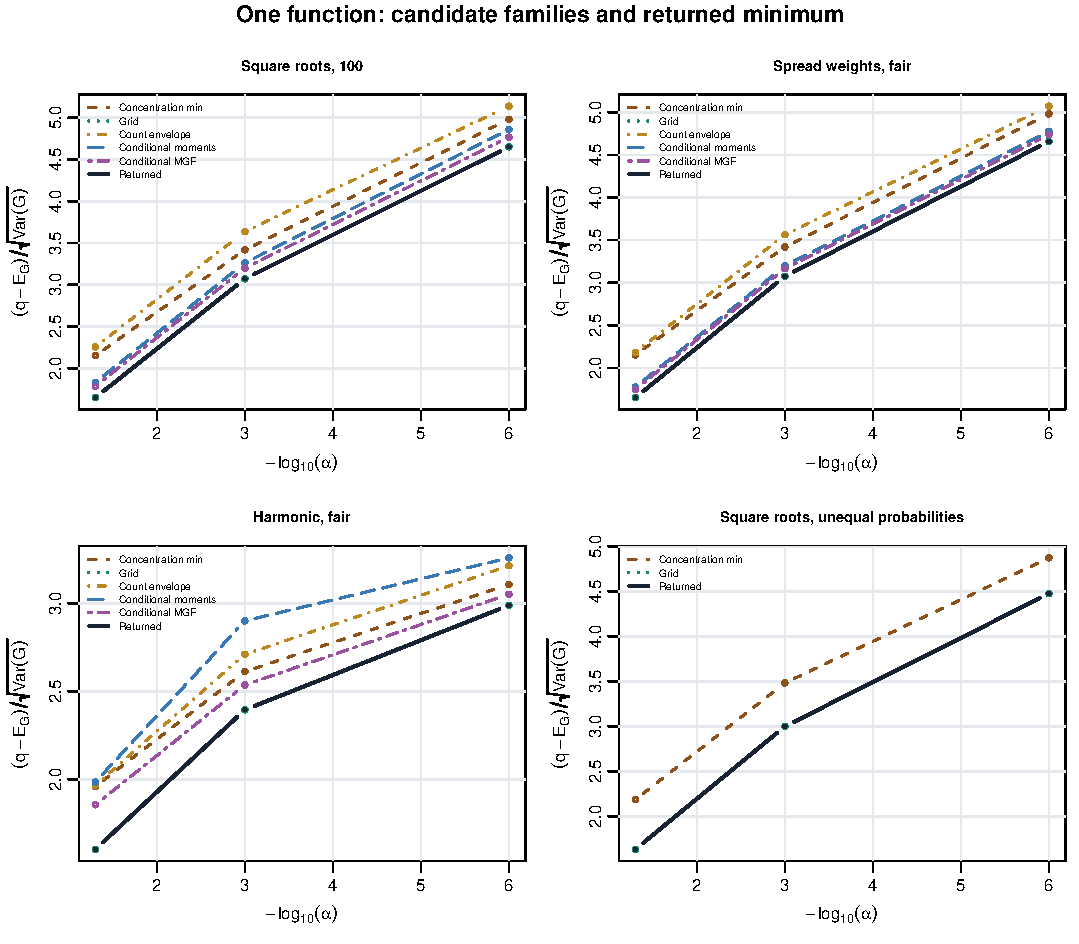
\includegraphics[width=\linewidth]{figures/bound_curves.pdf}
\caption{Candidate-family quantiles and the returned minimum in four
settings. Values are standardized by the true mean and standard deviation.
Lines connect only the three evaluated levels; they do not assert a
continuous interpolation guarantee. Some curves coincide because the
returned result is itself one of the plotted candidates.}
\label{fig:bound-curves}
\end{figure}

\begin{figure}[htbp]
\centering
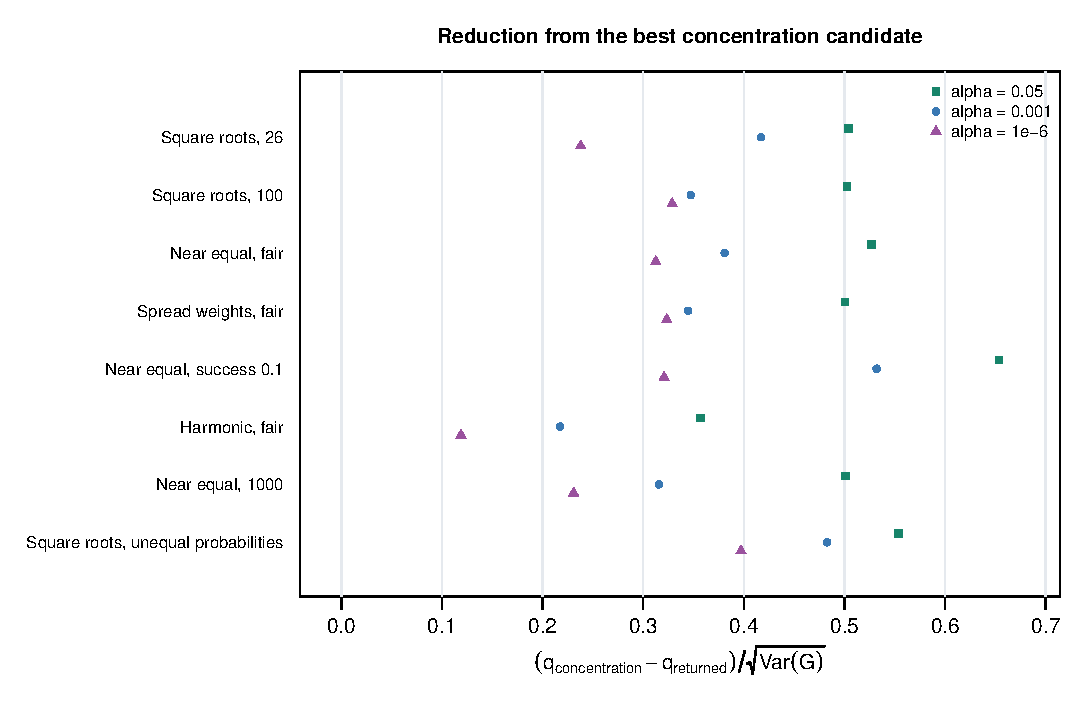
\includegraphics[width=\linewidth]{figures/improvement.pdf}
\caption{Reduction in the returned quantile relative to the smallest
ordinary concentration candidate, measured in standard deviations. Only
settings using the conservative branch appear. This compares deterministic
bounds with one another and does not require an independently known true
quantile.}
\label{fig:improvement}
\end{figure}

\subsection{Individual concentration bounds and achieved tails}

The Gaussian and Montgomery-Smith refinements remain part of the
calculation even when a numerical distribution surrogate wins. To inspect
them, filter the same diagnostic table rather than request a separate
concentration-only public method:
\par\noindent\begin{minipage}{\linewidth}
\begin{lstlisting}[language=R]
fit <- qweighted_bernoulli(
  0.05, 1 / (1:100), lower.tail = FALSE, details = TRUE
)
subset(fit$bounds,
       available & method %in% c("chernoff", "bentkus_gaussian",
                                "bentkus_gaussian_k", "pinelis_k"),
       select = c("method", "quantile", "selected"))
\end{lstlisting}
\end{minipage}\par

\begin{table}[htbp]
\centering
\small
\begin{tabular}{lrr}
\toprule
Individual candidate & Square roots, 100 & Harmonic, 100 \\
\midrule
Chernoff & 422.1244 & 3.8866 \\
Hoeffding & 422.7040 & 4.1586 \\
Cantelli & 490.6105 & 5.1874 \\
Bernstein & 427.8401 & 4.7356 \\
P2 & 414.1387 & 4.2667 \\
BD & 412.1675 & 3.9690 \\
K-BD & -- & 3.8466 \\
Pinelis & 413.9186 & 4.0005 \\
K-Pinelis & -- & 3.8667 \\
Sym. Chebyshev & 448.0925 & 4.6154 \\
Support & 671.4629 & 5.1874 \\
\bottomrule
\end{tabular}

\caption{Individual concentration candidates at $\alpha=0.05$. These are
component bounds, not the public function's final output. A missing
$K$-functional row can mean the decomposition adds no improvement over its
unsplit comparison. The returned minimum also includes the numerical
candidates in Table~\ref{tab:family-comparison}.}
\label{tab:concentration-components}
\end{table}

A valid upper quantile bound need not use the entire tail budget. For an
exact discrete quantile this already follows from its atom, and a
conservative candidate can leave additional probability unused.
Table~\ref{tab:actual-tails} computes the achieved strict tails directly
from independent reference distributions. The target is
$\Pr(G>\widehat q)\le\alpha$; replacing the strict inequality by an
inclusive one would count the boundary atom and change the comparison.

\begin{table}[htbp]
\centering
\footnotesize
\setlength{\tabcolsep}{3.3pt}
\begin{tabular}{llrrrl}
\toprule
Setting & $\alpha$ & Reference & Returned & Actual tail/$\alpha$ & Engine \\
\midrule
Equal, fair & 0.05 & 58.000 & 58.000 & 0.886 & Binomial \\
Equal, fair & $10^{-6}$ & 73.000 & 73.000 & 0.834 & Binomial \\
60 + 39 unit weights & 0.05 & 83.000 & 83.000 & 0.998 & Count classes \\
60 + 39 unit weights & $10^{-6}$ & 93.000 & 93.000 & 0.607 & Count classes \\
Near equal, fair & 0.05 & 58.096 & 58.124 & 0.974 & Grid \\
Near equal, fair & $10^{-6}$ & 73.160 & 73.195 & 0.935 & Grid \\
Spread weights, fair & 0.05 & 58.571 & 58.598 & 0.989 & Grid \\
Spread weights, fair & $10^{-6}$ & 74.222 & 74.256 & 0.966 & Grid \\
Near equal, success 0.1 & 0.05 & 15.053 & 15.060 & 0.985 & Grid \\
Near equal, success 0.1 & $10^{-6}$ & 26.914 & 26.928 & 0.971 & Grid \\
\bottomrule
\end{tabular}

\caption{Returned quantiles and achieved strict-tail ratios from independent
finite-law references. A ratio below one measures unused tail budget;
it is not an error in the exact quantile convention.}
\label{tab:actual-tails}
\end{table}

\subsection{Changing a resource limit still returns the minimum}

Table~\ref{tab:grid-resolution} changes only the lattice-state cap for
$w_i=\sqrt{i}$, $B=100$, at $\alpha=0.05$. The same function still evaluates
the other applicable candidates. The grid column is the internal grid
candidate, whereas ``Returned'' is the overall minimum. A coarse grid
therefore does not force the public answer to use that grid when another
candidate is smaller.

\begin{table}[htbp]
\centering
\small
\begin{tabular}{rrrrl}
\toprule
State cap & Grid candidate & Grid allowance & Returned & Selected engine \\
\midrule
512 & 446.0000 & 88.53705 & 399.1570 & Conditional MGF \\
8192 & 397.0000 & 4.78705 & 397.0000 & Grid \\
262144 & 394.3164 & 0.20893 & 394.3164 & Grid \\
\bottomrule
\end{tabular}

\caption{Grid state-budget study with the dynamic-programming work cap
fixed at its default $2\times10^7$. The grid allowance is its deterministic
absolute quantile-error bound plus numerical allowance. No method selector
is used in any row.}
\label{tab:grid-resolution}
\end{table}

\par\noindent\begin{minipage}{\linewidth}
\begin{lstlisting}[language=R]
fit <- qweighted_bernoulli(
  0.05, sqrt(1:100), lower.tail = FALSE, details = TRUE,
  control = list(max_states = 512)
)
fit$summary
subset(fit$bounds, method == "grid",
       select = c("quantile", "grid_error", "selected"))
\end{lstlisting}
\end{minipage}\par
The work caps are computational limits, not a user choice among competing
quantile methods. Increasing one cap can permit a sharper candidate, but
the cost and automatic partition choices should be assessed through the
reported diagnostics.

\subsection{Reproduction and validation}

There are 42 setting--level comparisons in the main run: 18 exact and
24 conservative returned values. Eight settings have independent reference
laws, yielding 261 individual candidate-tail checks. All returned
conservative values are checked against the minimum available diagnostic
candidate. Exact values are compared with the available independent
reference distributions, and every available candidate with such a
reference is checked using
\[
 \Pr(G>Q_j)\le \text{reported bound}_j(1+10^{-10})+10^{-15}.
\]
The file \texttt{results/validation.txt} records the actual counts, and
\texttt{results/all\_bounds.csv} includes available and skipped candidates,
partition labels, work counts, and reasons.

The separate regression script passed 708 checks across 25 categories.
These include 324 fair-binomial CDF atoms, 192 arbitrary-weight CDF-atom
and neighboring-level checks, mandatory exact behavior at length 25,
the minimum rule at length 26, structured exact calculations above 25,
tiny and subnormal success probabilities, extreme log tails, and 132
candidate-tail checks against exhaustive distributions. The record is
\texttt{results/unified\_validation.csv}. These checks are deterministic;
no Monte Carlo test is used to justify a probability bound.

The scripts run with standard R packages only \citep{rcore2026}. The
supplied run used WebR 0.6.0 with R 4.6.0 on
\texttt{wasm32-unknown-emscripten}; its session information is included.
Elapsed times in the CSV refer to one call with the three requested
levels. They describe this runtime and should not be read as native R
performance claims. The proofs establish the underlying conservative
formulas, while the numerical checks address implementation behavior.

\section{Recovering the randomized symmetric cutoff}
\label{sec:randomized}

This section connects ordinary quantiles to the original randomized
construction.  Assume $\pi_i=1/2$, retain nonnegative weights, and put
$W=\sum_{i=1}^B w_i$. In the original notation, $w_i=h(i)$,
$W=N_h=\sum_i h(i)$, and $G=G_{B,h}$.
Complementing every Bernoulli variable gives
$G\overset{d}=W-G$.  Define the folded statistic
\[
 C=\min\{G,W-G\}
   =\frac W2-\left|G-\frac W2\right|,
 \qquad 0\le C\le W/2.
\]
Its support is precisely
$\operatorname{supp}(G)\cap[0,W/2]$.  Adjoin the no-rejection sentinel
$-1$ and assign it CDF value zero, so that
$\mathcal S_h=\{-1\}\cup\operatorname{supp}(C)$.

\begin{proposition}[Folded quantile and exact randomization]
\label{prop:randomized-cutoff}
For every lower-half support point $c$,
\begin{equation}
 P_h(c):=\mathbb P\!\left(
  \left|G-\frac W2\right|\ge\frac W2-c\right)
 =\mathbb P(C\le c)
 =\begin{cases}
   2F_G(c),&c<W/2,\\
   1,&c=W/2.
  \end{cases}
 \label{eq:folded-cdf}
\end{equation}
Equivalently, $P_h(c)=\min\{1,2F_G(c)\}$ on that support.
For $0<\alpha<1$,
\begin{equation}
 c_+=q_C(\alpha)=q_G(\alpha/2).
 \label{eq:folded-ordinary-quantile}
\end{equation}
Let $c_-$ be the predecessor of $c_+$ in
$\{-1\}\cup\operatorname{supp}(C)$, with $P_h(-1)=0$.  Then
\begin{equation}
 \tau_{h,\alpha}
 =\frac{\alpha-P_h(c_-)}{P_h(c_+)-P_h(c_-)}\in(0,1].
 \label{eq:randomized-weight}
\end{equation}
If a variable $U\sim\operatorname{Unif}(0,1)$ is independent of $G$ and
of all data used in the rejection rule, set
\[
 \kappa=\begin{cases}
  c_+,&U\le\tau_{h,\alpha},\\
  c_-,&U>\tau_{h,\alpha}.
 \end{cases}
\]
Then $\mathbb P(C\le\kappa)=\alpha$ exactly.
\end{proposition}

\begin{proof}
The event $C\le c$ is
$\{G\le c\}\cup\{G\ge W-c\}$.  Below the midpoint these events are
disjoint and have equal probabilities by symmetry, giving
\eqref{eq:folded-cdf}.  At the midpoint their union is the whole sample
space, so a midpoint atom is counted only once.

Since $F_G(W/2)\ge1/2>\alpha/2$, the quantile $q_G(\alpha/2)$ is in
the lower half of the support.  Every smaller lower-half support point
$c$ satisfies $F_G(c)<\alpha/2$ and hence $P_h(c)<\alpha$.  At the
quantile, either it is below $W/2$ and $P_h(c)\ge\alpha$ follows by
doubling, or it equals $W/2$ and $P_h(c)=1$.  This proves
\eqref{eq:folded-ordinary-quantile}, including central support gaps and
midpoint atoms.  The predecessor definition implies
$P_h(c_-)<\alpha\le P_h(c_+)$, so the denominator in
\eqref{eq:randomized-weight} is positive and its ratio belongs to
$(0,1]$.  Finally, independence permits conditioning on the two values
of $\kappa$:
\[
 \mathbb P(C\le\kappa)
 =\tau_{h,\alpha}P_h(c_+)
 +(1-\tau_{h,\alpha})P_h(c_-)=\alpha.
\]
\end{proof}

The following straight-line calculation recovers the complete randomized
law when a finite PMF is available. The vector \texttt{s} contains support values for $G$,
\texttt{mass} contains their nonnegative masses, and \texttt{W} is the
sum of the original weights.  Repeated folded values are grouped and
their masses added.  This handles both the midpoint atom and ties caused
by different subsets with the same sum.  Input masses may be proportional
to probabilities; they are normalized at the start. This is a calculation
for a supplied PMF, rather than an additional quantile-function interface.
The first four lines specify a two-unit-weight example and can be replaced
by the support, masses, weight total, and target levels of interest.
\par\noindent\begin{minipage}{\linewidth}
\begin{lstlisting}[language=R]
s <- c(0, 1, 2)
mass <- c(1, 2, 1) / 4
W <- 2
alpha <- 0.75

stopifnot(length(s) == length(mass), length(s) > 0L,
          all(is.finite(s)), all(is.finite(mass)),
          all(mass >= 0), sum(mass) > 0,
          length(W) == 1L, is.finite(W), W >= 0,
          all(s >= 0 & s <= W),
          all(is.finite(alpha)), all(alpha > 0 & alpha < 1))
keep <- mass > 0
folded <- pmin(s[keep], W - s[keep])
mass <- mass[keep] / sum(mass[keep])
o <- order(folded)
folded <- folded[o]
mass <- mass[o]
first <- c(TRUE, diff(folded) != 0)
support <- folded[first]
folded_mass <- as.numeric(rowsum(mass, cumsum(first), reorder = FALSE))
F <- cumsum(folded_mass)
F[length(F)] <- 1
j <- vapply(alpha, function(a) which(F >= a)[1L], integer(1))
P_plus <- F[j]
P_minus <- c(0, F)[j]
cal <- data.frame(
  alpha = alpha, c_plus = support[j], c_minus = c(-1, support)[j],
  tau = (alpha - P_minus) / (P_plus - P_minus),
  P_minus = P_minus, P_plus = P_plus
)
\end{lstlisting}
\end{minipage}\par

For instance, with two unit weights the folded mass is $1/2$ at zero
and $1/2$ at one.  At $\alpha=3/4$, one therefore selects each of those
two cutoffs with probability $1/2$:
\begin{lstlisting}[language=R]
cal[, c("c_plus", "c_minus", "tau")]
#   c_plus c_minus tau
# 1      1       0 0.5

# Draw the cutoff using fresh randomization independent of the data.
u <- stats::runif(nrow(cal))
kappa <- ifelse(u <= cal$tau, cal$c_plus, cal$c_minus)
\end{lstlisting}

The calculation groups exact equalities of represented support values; it does
not merge arbitrarily close real values.  As with the main quantile
function, a floating-point PMF is subject to numerical representation
of its support and masses.  An integer lattice gives a convenient exact
description of support ties.  Zero weights cause no difficulty; if all
weights are zero, $C=0$ almost surely and the formula returns
$(c_-,c_+,\tau)=(-1,0,\alpha)$.

\subsection{Why an ordinary upper quantile cannot simply be reflected}

For a symmetric discrete distribution, reflection exchanges a strict
CDF inequality with a non-strict one.  In particular, for $0<p<1$,
\begin{equation}
 W-q_G(1-p)
 =\max\{x\in\operatorname{supp}(G):F_G(x^-)\le p\}.
 \label{eq:quantile-reflection}
\end{equation}
Indeed, $F_G(W-x)=\mathbb P(G\ge x)=1-F_G(x^-)$, and minimizing $W-x$
is equivalent to maximizing $x$.  Equation
\eqref{eq:quantile-reflection} is generally different from $q_G(p)$.
For $G\sim\operatorname{Bernoulli}(1/2)$ at $p=1/2$, the two values
are one and zero, respectively.

If the ordinary-quantile function supplies a conservative upper quantile
$u$ with $\mathbb P(G>u)\le\alpha/2$, symmetry gives only
\[
 \mathbb P(G<W-u)\le\alpha/2.
\]
Thus a lower cutoff $c<W-u$, with $c<W/2$, is safe for the inclusive
event $G\le c$; equality $c=W-u$ requires a separate check of the atom.
For a known lattice $\delta\mathbb Z$, one may choose
\begin{equation}
 c=\delta\left(\left\lceil\frac{W-u}{\delta}\right\rceil-1\right)
 \label{eq:strict-lattice-reflection}
\end{equation}
and replace a negative value by the sentinel $-1$.  The lattice point in
\eqref{eq:strict-lattice-reflection} need not be an attainable subset sum,
but its event is well defined and has probability at most $\alpha$ after
folding.  If a concentration calculation instead explicitly certifies
the inclusive upper event $\mathbb P(G\ge u)\le\alpha/2$, equality
$c=W-u<W/2$ is permitted.  The public function's general contract is
the strict-tail statement \eqref{eq:strict-quantile-tail}; an inclusive
certificate must therefore be established separately.

For integer weights, the conservative nonrandomized lower cutoff is computed
as follows. The two-sided target is \texttt{alpha}; the ordinary quantile
call uses its one-sided half.
\begin{lstlisting}[language=R]
w <- 1:100
alpha <- 0.05
upper <- qweighted_bernoulli(
  alpha / 2, weights = w, lower.tail = FALSE
)
c_safe <- ceiling(sum(w) - upper) - 1
if (c_safe < 0) c_safe <- -1
# Reject when min(G, sum(w) - G) <= c_safe.
\end{lstlisting}
This is a conservative rejection rule. It does not claim to recover the
canonical randomized law of Proposition~\ref{prop:randomized-cutoff}.

Finally, a conservative upper bound for $q_G(\alpha/2)$ cannot be used
as $c_+$ with the same randomization formula unless the associated
probabilities are also available.  Enlarging a lower rejection cutoff
increases its rejection probability.  The ordinary-quantile function
and the folded-PMF construction solve related but distinct inversion
problems, and the latter is the route that recovers the canonical
$c_-,c_+,\tau_{h,\alpha}$ exactly.

\section{Numerical precision, work limits, and reproducibility}
\label{sec:numerical-resources}

\subsection{What exact and conservative mean in the implementation}

All stochastic comparisons and quantile inequalities in this note are
statements in real arithmetic. An exact distribution algorithm removes
an approximation to the probability law, but its R implementation still
uses rounded additions, multiplications, and support comparisons. This
matters at or very near a CDF jump. The function preserves ordinary-scale
input probabilities when useful, evaluates small tails directly, checks
support boundaries, and switches to logarithmic probabilities when masses
would underflow. In particular, it never identifies the zero endpoint by
comparing two ordinary-scale probabilities that have both rounded to one
when a smaller upper-tail comparison is available.

The mandatory short-vector route has a log-domain meet-in-the-middle
calculation. A structural PMF calculation that cannot resolve a requested
extreme tail can pass that request to this exact route when the active
length is at most \texttt{max\_length}. If the requested exact calculation
cannot be resolved, it reports an error; it does not label an approximate
answer exact. Above the threshold an unresolved structural calculation
passes to the conservative collection instead of generic enumeration.

For conservative calculations, positive weights are rescaled by a power
of two before variances and generating functions are formed. This reduces
overflow risk. A term whose normalized weight is smaller than the smallest
positive normal floating-point number is replaced, for these normalized
bound calculations, by its deterministic maximum contribution. This
preserves an upper quantile bound. Common-probability and fairness
hypotheses are then checked on the remaining random sum; the deterministic
contribution is added back. This numerical reduction does not change the
active count used for the exact-dispatch threshold. Upward grid construction checks
the represented rounding direction. Conservative thresholds receive small
positive numerical allowances, and inverse searches retain a feasible
upper bracket. These are numerical safeguards, not a complete outward
error analysis of R's mathematical library.

Consequently, ``exact'' means an exact finite-distribution algorithm
evaluated in double precision. The conservative results implement the
proved formulas with the same numerical qualification. A formal
machine-verifiable certificate at a CDF boundary would require certified
interval or exact rational arithmetic for probabilities and special
functions. The reproducible checks below test numerical implementation;
they do not replace the proofs or turn double precision into such a
certificate.

There is a useful representable subcase: at most 52 active fair Bernoulli
variables on a represented integer lattice have dyadic PMF and cumulative
probabilities that the array recurrence can represent exactly, as proved
in Section~\ref{sec:exact-grid}. General success probabilities and arbitrary
real subset sums need not have that property.

\subsection{The exact threshold and the resource controls}

\texttt{max\_length = 25} controls whether generic exact subset-sum
computation is requested. It is separate from the work controls. For a
required exact calculation with $n\le25$ active terms, the implementation
allows at least $2^{\lceil n/2\rceil}$ entries per half-array and at least
2200 support-search iterations, and does not impose the
\texttt{max\_mitm\_work} query cap. Thus reducing conservative work budgets
does not silently change this exact request into a bound. A user who
raises \texttt{max\_length} above 25 is requesting a potentially larger
exact calculation; cases with $n>25$ use the specified exact work limits.
If a required exact calculation cannot be resolved, the function reports
an error.

The conservative and structural work limits are finite. They avoid a long
nonlattice vector accidentally initiating an unrestricted enumeration.
The defaults are:
\begin{lstlisting}[language=R]
control <- list(
  max_states = 2^18,
  max_dp_work = 2e7,
  max_mitm_work = 2e7,
  max_iterations = 80,
  chernoff_iterations = 60,
  max_p2_B = 10000,
  max_p2_work = 200000,
  max_group_states = 65536,
  max_count_states = 100000,
  max_mgf_work = 2e7,
  mgf_points = 37
)
\end{lstlisting}
Ordinary use does not require supplying this list. To adjust a resource,
pass only the named entries to change:
\begin{lstlisting}[language=R]
fit <- qweighted_bernoulli(
  c(0.05, 0.01), weights = sqrt(1:100), lower.tail = FALSE,
  details = TRUE, control = list(max_states = 2^19)
)
fit$summary
\end{lstlisting}

\begin{table}[htbp]
\centering
\small
\caption{Resource controls. Counts are work proxies, not elapsed-time or
byte-allocation promises.}
\label{tab:controls}
\begin{tabularx}{\linewidth}{@{}lX@{}}
\toprule
Control & Role \\
\midrule
\texttt{max\_states} & Lattice-array or meet-in-the-middle half-array cap;
the required $n\le25$ exact branch raises the latter if necessary. \\
\texttt{max\_dp\_work} & Sum of intermediate array lengths for one
PMF calculation; also determines an affordable upward grid. \\
\texttt{max\_mitm\_work} & Visited left-half entries in generic exact
support queries. This cap is not imposed for a required $n\le25$ exact
calculation. \\
\texttt{max\_iterations} & Budget for scalar searches and bound inversions;
the mandatory short exact route uses a larger floor when necessary. \\
\texttt{chernoff\_iterations} & Generating-function optimization evaluations
per distinct level. \\
\texttt{max\_p2\_B}, \texttt{max\_p2\_work} & Active-count and preparation/scan
limits for the binomial $P_2$ candidate. \\
\texttt{max\_group\_states} & Enumerated non-pivot states for a grouped
count envelope or an exact repeated-class representation. \\
\texttt{max\_count\_states} & Full joint count-state cap for conditional
moment and generating-function calculations. \\
\texttt{max\_mgf\_work} & Conditional generating-function preparation and
joint-table work cap, applied separately to each candidate partition. \\
\texttt{mgf\_points} & Total number of points in the automatic conditional
MGF grid, including zero. The default 37 means zero and 36 positive points. \\
\bottomrule
\end{tabularx}
\end{table}

Controls are integer-valued. The optional $P_2$, grouped, conditional-count,
and MGF budgets may be zero; zero disables the corresponding calculation.
Other controls are positive, with \texttt{mgf\_points}\,$\ge2$.
Each of the three state caps must be at most $2^{30}$.

The lattice recurrence takes $O(\sum_j(S_j+1))$ operations and
$O(S_B+1)$ memory. A balanced meet-in-the-middle representation stores
$O(2^{B/2})$ entries and makes sorted-array probability queries. At $B=25$
the two half-array sizes are only 4096 and 8192, although query work also
depends on the number of requested levels and support searches.

After moments are prepared, elementary and Gaussian bounds cost constant
work per level apart from scalar inversion. The $K$-functional uses sorted
weights and cumulative squares. Chernoff costs $O(BI)$ per level for a
fixed iteration budget $I$. The binomial $P_2$ preparation and each scan
cost $O(B)$, with prepared arrays shared across the requested levels.

For groups of sizes $m_j$, the grouped count envelope enumerates
$\prod_j(m_j+1)/\max_j(m_j+1)$ states and integrates the largest group
using its binomial CDF. The conditional calculation stores the full
$\prod_j(m_j+1)$ states. With one group this is only $B+1$. Conditional
MGF tables cost $O(|\Lambda|\sum_jm_j^2)$ to prepare; joint evaluation
also depends on $|\Lambda|\prod_j(m_j+1)$.

\paragraph{Automatic partitions and MGF parameters.}
For a common active success probability, the implementation considers a
fixed collection of inexpensive partitions: one full group, two or three
ordered blocks, partitions retaining a few largest weights as singletons,
and an affordable greedy refinement. Duplicate partitions are removed.
The grouped-envelope and conditional engines have different state caps,
so a partition can be available for one and skipped for the other.
For a positive largest within-group weight spread $R$, the default MGF
parameter grid consists of zero and 36 logarithmically spaced points from
$0.01/R$ to $500/R$. Thus \texttt{mgf\_points=37} counts zero as well.
These parameters are expressed in the original weight units in the
diagnostics. This is an explicit finite numerical family, not an exact
continuous minimization.
The minimum with all other candidates preserves validity if an MGF table
or a partition is skipped. Details of the actual partitions and work
limits are included in the returned diagnostics.

The mathematical improvement under a nested refinement of groups is
proved in Section~\ref{sec:aggregation}. Changing an automatic work budget
can also change which partitions and parameter grids are examined.
Accordingly, that theorem should not be read as a promise that every
heuristic budget change produces a monotone sequence of returned numbers.

\subsection{Error allowances and interpretation of diagnostics}

When a grid candidate has upper quantile $Q_{\rm grid}$ and deterministic
rounding allowance $\Delta$, the coupling proves
$q_G(p)\ge Q_{\rm grid}-\Delta$. If another valid candidate is smaller,
$Q_{\rm grid}-\Delta$ is still a lower certificate for comparison with the
selected upper value. Grouped lower envelopes give further lower
certificates. Whenever they are available, one may combine them as
\[
 \ell=\max\{Q_{\rm grid}-\Delta,\ Q^-_{\rm group},\ldots\}
 \le q_G(p)\le \widehat q.
\]
The resulting gap is $\widehat q-\ell$; there is no need to treat the
selected upper bound as a grid calculation. More generally, a candidate
row with quantile $Q_j$ and finite error allowance $E_j$ supplies the
lower bound $Q_j-E_j$. The candidate table therefore permits this
additional comparison even when the selected row has no error allowance;
the function does not currently return the combined value $\ell$.

The retained diagnostic field \texttt{grid\_error} records the explicit
absolute allowance of a selected grid or grouped-envelope candidate,
including its numerical search allowance. It is zero for an exact answer
and is \texttt{NA} when a different conservative candidate wins. Individual candidate
rows retain their own allowances; the field name does not make a
conditional concentration result an exact distribution calculation.
The \texttt{reason} column records failed hypotheses or resource limits.
An unavailable candidate is omitted from the numerical minimum, while
its reason remains visible.

\subsection{Contents and reproduction}

The package contains one public implementation,
\texttt{qweighted\_bernoulli.R}; this file sources nothing else.
The full function is also printed in Appendix~\ref{sec:complete-function}.
The accompanying files are:
\begin{itemize}
\item \texttt{weighted\_bernoulli\_quantiles.pdf} and its LaTeX source;
\item \texttt{usage\_examples.R}, executable examples of the one interface;
\item \texttt{reproduce.R}, all settings, tables, and figures in
Section~\ref{sec:comparisons};
\item \texttt{verify\_quantiles.R}, independent regression checks;
\item \texttt{results/}, CSV data, generated tables, validation summaries,
and runtime information; and \texttt{figures/}, vector PDF figures.
\end{itemize}
Run from the extracted directory:
\begin{lstlisting}[language=R]
source("usage_examples.R")
source("reproduce.R")
source("verify_quantiles.R")
\end{lstlisting}
Alternatively use \texttt{Rscript} with each script filename. The scripts
may define local reference calculations for validation; they do not add
alternative public quantile functions. All numerical references are
finite-distribution calculations or explicitly labeled coupling brackets,
not Monte Carlo approximations. Runtime information is recorded in
\texttt{results/sessionInfo.txt}.

\FloatBarrier
\begin{thebibliography}{10}
\small

\bibitem{bardenetmaillard2015}
R. Bardenet and O.-A. Maillard (2015).
Concentration inequalities for sampling without replacement.
\emph{Bernoulli} \textbf{21}(3), 1361--1385.
\href{https://doi.org/10.3150/14-BEJ605}{doi:10.3150/14-BEJ605}.
\href{https://arxiv.org/abs/1309.4029}{arXiv:1309.4029}.

\bibitem{bennett1962}
G. Bennett (1962).
Probability inequalities for the sum of independent random variables.
\emph{Journal of the American Statistical Association} \textbf{57}(297),
33--45.
\href{https://doi.org/10.1080/01621459.1962.10482149}
{doi:10.1080/01621459.1962.10482149}.

\bibitem{bentkus2004}
V. Bentkus (2004).
On Hoeffding's inequalities.
\emph{The Annals of Probability} \textbf{32}(2), 1650--1673.
\href{https://doi.org/10.1214/009117904000000360}
{doi:10.1214/009117904000000360}.
\href{https://arxiv.org/abs/math/0410159}{arXiv:math/0410159}.

\bibitem{bentkusdzindzalieta2015}
V. K. Bentkus and D. Dzindzalieta (2015).
A tight Gaussian bound for weighted sums of Rademacher random variables.
\emph{Bernoulli} \textbf{21}(2), 1231--1237.
\href{https://doi.org/10.3150/14-BEJ603}{doi:10.3150/14-BEJ603}.
\href{https://arxiv.org/abs/1307.3451}{arXiv:1307.3451}.

\bibitem{bentkusjuskevicius2008}
V. Bentkus and T. Ju\v skevi\v cius (2008).
Bounds for tail probabilities of martingales using skewness and kurtosis.
\emph{Lithuanian Mathematical Journal} \textbf{48}, 30--37.
\href{https://doi.org/10.1007/s10986-008-0003-8}
{doi:10.1007/s10986-008-0003-8}.
\href{https://arxiv.org/abs/1111.6358}{arXiv:1111.6358}
(posted in 2011).

\bibitem{hoeffding1963}
W. Hoeffding (1963).
Probability inequalities for sums of bounded random variables.
\emph{Journal of the American Statistical Association} \textbf{58}(301),
13--30.
\href{https://doi.org/10.1080/01621459.1963.10500830}
{doi:10.1080/01621459.1963.10500830}.

\bibitem{hitczenkokwapien1994}
P. Hitczenko and S. Kwapie\'n (1994).
On the Rademacher series.
In J. Hoffmann-J\o rgensen, J. Kuelbs, and M. B. Marcus (eds.),
\emph{Probability in Banach Spaces, 9}, Progress in Probability
\textbf{35}, 31--36. Birkh\"auser, Boston.
\href{https://doi.org/10.1007/978-1-4612-0253-0_2}
{doi:10.1007/978-1-4612-0253-0\_2}.

\bibitem{hollomportier2025}
L. Hollom and J. Portier (2025).
Tight anti-concentration of Rademacher sums.
\emph{Random Structures \& Algorithms} \textbf{67}(1), article e70024.
\href{https://doi.org/10.1002/rsa.70024}{doi:10.1002/rsa.70024}.
\href{https://arxiv.org/abs/2306.07811}{arXiv:2306.07811}.

\bibitem{kellerklein2022}
N. Keller and O. Klein (2022).
Proof of Tomaszewski's conjecture on randomly signed sums.
\emph{Advances in Mathematics} \textbf{407}, article 108558.
\href{https://doi.org/10.1016/j.aim.2022.108558}
{doi:10.1016/j.aim.2022.108558}.
\href{https://arxiv.org/abs/2006.16834}{arXiv:2006.16834}.

\bibitem{pinelis2012}
I. Pinelis (2012).
An asymptotically Gaussian bound on the Rademacher tails.
\emph{Electronic Journal of Probability} \textbf{17}, article 35, 1--22.
\href{https://doi.org/10.1214/EJP.v17-2026}{doi:10.1214/EJP.v17-2026}.
\href{https://arxiv.org/abs/1007.2137}{arXiv:1007.2137}.

\bibitem{montgomerysmith1990}
S. J. Montgomery-Smith (1990).
The distribution of Rademacher sums.
\emph{Proceedings of the American Mathematical Society}
\textbf{109}(2), 517--522.
\href{https://doi.org/10.1090/S0002-9939-1990-1013975-0}
{doi:10.1090/S0002-9939-1990-1013975-0}.
\href{https://stephenmontgomerysmith.github.io/preprints/tail.pdf}
{Author's preprint}.

\bibitem{rcore2026}
R Core Team (2026).
\emph{R: A Language and Environment for Statistical Computing}.
R Foundation for Statistical Computing, Vienna, Austria.
\url{https://www.R-project.org/}.

\bibitem{rbinomial}
R Core Team (2026).
\emph{The Binomial Distribution}. R \texttt{stats} documentation.
\url{https://stat.ethz.ch/R-manual/R-devel/library/stats/html/Binomial.html}.
Accessed October 6, 2026.

\bibitem{rsignrank}
R Core Team (2026).
\emph{Distribution of the Wilcoxon Signed Rank Statistic}.
R \texttt{stats} documentation.
\url{https://stat.ethz.ch/R-manual/R-devel/library/stats/html/SignRank.html}.
Accessed October 6, 2026.

\end{thebibliography}

\clearpage
\appendix
\section{Complete standalone implementation}
\label{sec:complete-function}

The listing below is the complete contents of
\texttt{qweighted\_bernoulli.R}. It defines one public function; all helpers
are local. The implementation uses only base R and \texttt{stats}, and
sources no companion implementation files. Save the code in that filename
and use the calls in Section~\ref{sec:usage}. This is the same source used
for the numerical comparisons and regression checks.

\begin{lstlisting}[style=Rcode,basicstyle=\ttfamily\fontsize{7.7}{9.4}\selectfont,
  numbers=left,numberstyle=\tiny\color{CodeComment},stepnumber=10,
  numbersep=7pt]
# Quantiles of independent weighted Bernoulli sums: ONE public function.
# X = sum(weights[i] * Bernoulli(prob[i])); nonnegative finite weights.
# Only base R and stats are needed. All implementation helpers are local.
#
# qweighted_bernoulli(p, weights, prob=0.5, max_length=25,
#                    lower.tail=TRUE, log.p=FALSE, details=FALSE,
#                    control=list())
#
# The ordinary p-quantile is inf{x: Pr(X <= x) >= p}. At p=0 and p=1
# return the support endpoints. lower.tail=FALSE supplies Pr(X > q);
# log.p=TRUE supplies its logarithm. Names and vector probability inputs work.
#
# Automatic dispatch (no method selector):
# 1. Remove zero and deterministic terms. Recognize binomial, fair rank,
#    affordable exact lattice, and repeated (weight, probability) count laws.
# 2. For at most max_length active terms, compute an exact finite-distribution
#    quantile by meet-in-the-middle if necessary. The default max_length is 25.
# 3. Otherwise evaluate every applicable candidate within its documented work
#    limits and return their minimum: concentration, upward grid, grouped
#    count envelopes, conditional moments, and conditional MGF-grid bounds.
# The count bounds currently require one common active success probability.
#
# A conservative result satisfies Pr(X > q) <= the requested upper-tail level.
# This is a STRICT tail. A returned bound need not be a support point.
# Exact means an exact finite-distribution algorithm in double precision,
# not symbolic or certified interval arithmetic. Numerically indistinguishable
# subset sums and CDF jumps retain the usual floating-point qualification.
#
# details=TRUE returns quantile, summary, bounds, and diagnostics. For a bound
# calculation, bounds records every attempted candidate, its availability,
# reason, partition, and selected flag; summary always selects its minimum.
# Exact requests have exact=TRUE and bypass unnecessary conservative work.
# The minimum is over the implemented finite candidate/partition/lambda set,
# not over all possible partitions or all probability inequalities.
#
# control defaults (integer limits; zero disables the indicated optional route):
# max_states=2^18: lattice/grid states and one MITM half-array.
# max_dp_work=2e7: cumulative lattice/grid updates.
# max_mitm_work=2e7: visited left-half entries in exact probability queries.
# max_iterations=80: conservative and structured-exact inversions.
# chernoff_iterations=60: optimized MGF-Chernoff evaluations per level.
# max_p2_B=10000, max_p2_work=200000: optional binomial P2 budgets.
# max_group_states=65536: exact-block/grouped pivot remainder states.
# max_count_states=100000: conditional joint count states.
# max_mgf_work=2e7: conditional MGF preparation/array budget per partition.
# mgf_points=37: finite grid, zero plus 36 log-spaced positive lambdas.
# Optional P2, grouped, count, and MGF budgets may be zero. For <=25 active
# terms, the promised exact branch floors MITM storage, bypasses the query-work cap,
# and allows 2200 support-search iterations; restrictive controls cannot silently
# switch it to an approximation. Larger user-selected max_length values are
# subject to the stated exact work limits and cause an error if unresolved.
#
# Examples:
# qweighted_bernoulli(c(0.025, 0.5, 0.975), weights=sqrt(1:25))
# qweighted_bernoulli(0.95, c(100, rep(1, 999)), details=TRUE)
# qweighted_bernoulli(0.05, seq(0.99, 1.01, length.out=1000),
#                    lower.tail=FALSE, details=TRUE)
# qweighted_bernoulli(log(1e-30), sqrt(1:100),
#                    lower.tail=FALSE, log.p=TRUE)
#
# Primary references: Bentkus-Dzindzalieta, doi:10.3150/14-BEJ603;
# Pinelis, doi:10.1214/EJP.v17-2026; Bentkus, arXiv:math/0410159;
# Keller-Klein, arXiv:2006.16834; Montgomery-Smith,
# doi:10.1090/S0002-9939-1990-1013975-0; Bardenet-Maillard,
# doi:10.3150/14-BEJ605. The accompanying note derives the count refinements.

qweighted_bernoulli <- function(
    p, weights, prob=0.5, max_length=25,
    lower.tail=TRUE, log.p=FALSE, details=FALSE, control=list()) {

  log_complement <- function(x) {
    answer <- numeric(length(x))
    small <- x < -log(2)
    answer[small] <- log1p(-exp(x[small]))
    answer[!small] <- log(-expm1(x[!small]))
    answer
  }

  probability_upper <- function(x) {
    ifelse(is.infinite(x) & x < 0, 0, pmin(1, pmax(2^-1074, exp(x))))
  }


  # Internal exact engines for the stand-alone weighted Bernoulli quantile.
  # These local helpers take positive weights as inputs;
  # probabilities are strictly between zero and one. The public wrapper handles
  # deterministic terms and endpoints. Each engine returns a data.frame with
  # quantile, exact, and method, or NULL when its resource limits do not permit
  # computation. An NA quantile is an unresolved request that needs a fallback.
  # lower_prob / upper_prob preserve unlogged input levels at CDF jumps.

  exact_target_ok <- function(cdf, survival, j, log_lower, log_upper,
                              lower_prob = NULL, upper_prob = NULL) {
    if (log_lower[j] <= -log(2)) {
      if (!is.null(lower_prob)) return(cdf >= lower_prob[j])
      return(log(cdf) >= log_lower[j])
    }
    if (!is.null(upper_prob)) return(survival <= upper_prob[j])
    log(survival) <= log_upper[j]
  }

  exact_result <- function(q, method) {
    data.frame(quantile = q, exact = TRUE, method = method,
               stringsAsFactors = FALSE)
  }

  # No approximate rounding of arbitrary scores is used to recognize a lattice.
  exact_lattice <- function(w) {
    integer_gcd <- function(a, b) {
      while (b != 0) {
        r <- a %% b
        a <- b
        b <- r
      }
      a
    }
    step <- min(w)
    z <- w / step
    if (all(is.finite(z)) && all(z == floor(z)) &&
        max(z) <= 2^52 && all(step * z == w) && sum(z) <= 2^52) {
      return(list(weights = z, step = step))
    }
    # Power-of-two scaling also recognizes, for example, weights (1, 1.5).
    # Try binary units without changing the represented input weights.
    exponent <- max(-1022, min(1023, floor(log2(max(w)))))
    step <- 2^exponent
    z <- w / step
    for (iteration in 0:52) {
      if (any(!is.finite(z)) || max(z) > 2^52) break
      if (all(z == floor(z)) && all(z > 0)) {
        g <- Reduce(integer_gcd, z)
        z <- z / g
        step <- step * g
        if (sum(z) <= 2^52 && all(z * step == w)) {
          return(list(weights = z, step = step))
        }
        break
      }
      z <- z * 2
      step <- step / 2
      if (step == 0) break
    }
    NULL
  }

  # Full lattice DP is also exposed for the wrapper's upward-rounded grid.
  # Its returned quantiles are in integer lattice coordinates.
  dp_quantiles <- function(w_integer, prob, log_lower, log_upper, control,
                           lower_prob = NULL, upper_prob = NULL) {
    ordering <- order(w_integer)
    w_integer <- w_integer[ordering]
    prob <- prob[ordering]
    total <- sum(w_integer)
    if (!is.finite(total) || total + 1 > control$max_states ||
        sum(1 + cumsum(w_integer)) > control$max_dp_work) return(NULL)
    if (any(w_integer < 1 | w_integer != floor(w_integer))) return(NULL)
    mass <- 1
    for (j in seq_along(w_integer)) {
      a <- w_integer[j]
      old <- seq_along(mass)
      next_mass <- numeric(length(mass) + a)
      next_mass[old] <- mass * (1 - prob[j])
      next_mass[old + a] <- next_mass[old + a] + mass * prob[j]
      mass <- next_mass
    }
    cdf <- cumsum(mass)
    # survival[k + 1] = P(sum > k), evaluated without 1 - CDF.
    survival <- c(rev(cumsum(rev(mass[-1L]))), 0)
    answer <- rep(NA_real_, length(log_lower))
    for (j in seq_along(answer)) {
      # Ordinary arithmetic is inappropriate for targets near probability
      # underflow. The public function may use a bound for these requests.
      if (min(log_lower[j], log_upper[j]) < -650) next
      ok <- function(k) exact_target_ok(cdf[k], survival[k], j,
        log_lower, log_upper, lower_prob, upper_prob)
      lo <- 1L
      hi <- length(mass)
      if (!ok(hi)) next
      while (lo < hi) {
        mid <- floor(lo + (hi - lo) / 2)
        if (ok(mid)) hi <- mid else lo <- mid + 1L
      }
      if (ok(lo) && (lo == 1L || !ok(lo - 1L))) answer[j] <- lo - 1
    }
    exact_result(answer, "lattice_dp")
  }

  # Correct the quantile routine's deliberate fuzz by checking the CDF jump.
  # The binary correction costs O(log(number of support points)) CDF calls.
  exact_standard_quantiles <- function(n, step, success, kind,
                                       log_lower, log_upper, control,
                                       lower_prob = NULL, upper_prob = NULL) {
    total <- if (kind == "binomial") n else n * (n + 1) / 2
    distribution <- if (kind == "binomial") {
      function(k, lower.tail, log.p) stats::pbinom(k, n, success,
        lower.tail = lower.tail, log.p = log.p)
    } else {
      function(k, lower.tail, log.p) stats::psignrank(k, n,
        lower.tail = lower.tail, log.p = log.p)
    }
    quantile <- if (kind == "binomial") {
      function(p, lower.tail) stats::qbinom(p, n, success,
        lower.tail = lower.tail, log.p = TRUE)
    } else {
      function(p, lower.tail) stats::qsignrank(p, n,
        lower.tail = lower.tail, log.p = TRUE)
    }
    if (kind == "binomial" && success == 0.5 && n <= 52L) {
      row <- 1
      for (j in seq_len(n)) row <- c(row, 0) + c(0, row)
      cdf <- cumsum(row) * 2^-n
      survival <- c(rev(cumsum(rev(row[-1L]))), 0) * 2^-n
      distribution <- function(k, lower.tail, log.p) {
        at <- pmin(n, pmax(0, floor(k))) + 1L
        value <- if (lower.tail) cdf[at] else survival[at]
        value[k < 0] <- if (lower.tail) 0 else 1
        value[k >= n] <- if (lower.tail) 1 else 0
        if (log.p) log(value) else value
      }
    }
    answer <- rep(NA_real_, length(log_lower))
    for (j in seq_along(answer)) {
      lower <- log_lower[j] <= -log(2)
      ok <- if (lower) {
        if (is.null(lower_prob)) {
          function(k) distribution(k, TRUE, TRUE) >= log_lower[j]
        } else {
          function(k) distribution(k, TRUE, FALSE) >= lower_prob[j]
        }
      } else {
        if (is.null(upper_prob)) {
          function(k) distribution(k, FALSE, TRUE) <= log_upper[j]
        } else {
          function(k) distribution(k, FALSE, FALSE) <= upper_prob[j]
        }
      }
      q <- quantile(if (lower) log_lower[j] else log_upper[j], lower)
      if (!is.finite(q)) next
      q <- min(total, max(0, q))
      lo <- 0
      hi <- total
      if (!ok(q)) {
        lo <- q + 1
      } else if (q > 0 && ok(q - 1)) {
        hi <- q - 1
      } else {
        lo <- hi <- q
      }
      if (lo > hi) next
      for (iteration in seq_len(control$max_iterations)) {
        if (lo >= hi) break
        mid <- floor(lo + (hi - lo) / 2)
        if (ok(mid)) hi <- mid else lo <- mid + 1
      }
      if (lo == hi && ok(lo) && (lo == 0 || !ok(lo - 1))) {
        answer[j] <- step * lo
      }
    }
    exact_result(answer, kind)
  }

  exact_half_distribution <- function(w, prob) {
    values <- 0
    mass <- 1
    log_mass <- 0
    for (j in seq_along(w)) {
      values <- c(values, values + w[j])
      mass <- c(mass * (1 - prob[j]), mass * prob[j])
      log_mass <- c(log_mass + log1p(-prob[j]), log_mass + log(prob[j]))
    }
    ordering <- order(values)
    list(values = values[ordering], mass = mass[ordering],
         log_mass = log_mass[ordering])
  }

  exact_mitm_quantiles <- function(w, prob, log_lower, log_upper, control,
                                  lower_prob = NULL, upper_prob = NULL) {
    n <- length(w)
    if (n > min(52, control$mitm_B) ||
        2^ceiling(n / 2) > control$max_states) return(NULL)
    m <- floor(n / 2)
    left <- exact_half_distribution(w[seq_len(m)], prob[seq_len(m)])
    right_indices <- seq.int(m + 1L, n)
    right <- exact_half_distribution(w[right_indices], prob[right_indices])
    a <- left$values
    b <- right$values
    nb <- length(b)
    prefix <- c(0, cumsum(right$mass))
    suffix <- c(rev(cumsum(rev(right$mass))), 0)
    use_log <- any(pmin(log_lower, log_upper) < -650)
    log_add <- function(x, y) {
      z <- max(x, y)
      if (!is.finite(z)) return(z)
      z + log1p(exp(-abs(x-y)))
    }
    log_sum <- function(x) {
      z <- max(x)
      if (!is.finite(z)) return(z)
      z + log(sum(exp(x-z)))
    }
    if (use_log) {
      log_prefix <- log_suffix <- rep(-Inf, nb + 1L)
      for (j in seq_len(nb))
        log_prefix[j + 1L] <- log_add(log_prefix[j], right$log_mass[j])
      for (j in rev(seq_len(nb)))
        log_suffix[j] <- log_add(log_suffix[j + 1L], right$log_mass[j])
    }
    used <- 0
    maximum <- max(a) + max(b)
    cache <- new.env(parent = emptyenv())

    pairs <- function(x, strict = FALSE) {
      used <<- used + length(a)
      if (used > control$max_mitm_work) return(NULL)
      j <- findInterval(x - a, b)
      bad <- logical(length(a))
      ii <- which(j > 0L)
      v <- a[ii] + b[j[ii]]
      bad[ii] <- if (strict) v >= x else v > x
      ii <- which(j < nb)
      v <- a[ii] + b[j[ii] + 1L]
      bad[ii] <- bad[ii] | if (strict) v < x else v <= x
      ii <- which(bad)
      if (length(ii)) {
        # Repair subtraction/addition rounding disagreements. This also
        # moves to the correct edge of a repeated subset-sum value.
        lower <- integer(length(ii))
        upper <- rep.int(nb + 1L, length(ii))
        active <- seq_along(ii)
        while (length(active)) {
          mid <- floor((lower[active] + upper[active]) / 2)
          v <- a[ii[active]] + b[mid]
          good <- if (strict) v < x else v <= x
          lower[active[good]] <- mid[good]
          upper[active[!good]] <- mid[!good]
          active <- which(upper - lower > 1L)
        }
        j[ii] <- lower
      }
      list(cdf = sum(left$mass * prefix[j + 1L]),
           survival = sum(left$mass * suffix[j + 1L]),
           log_cdf = if (use_log)
             min(0, log_sum(left$log_mass + log_prefix[j + 1L])) else NULL,
           log_survival = if (use_log)
             min(0, log_sum(left$log_mass + log_suffix[j + 1L])) else NULL,
           j = j)
    }

    answer <- rep(NA_real_, length(log_lower))
    for (k in seq_along(answer)) {
      lower <- log_lower[k] <= -log(2)
      target <- if (lower) {
        if (is.null(lower_prob)) log_lower[k] else lower_prob[k]
      } else {
        if (is.null(upper_prob)) log_upper[k] else upper_prob[k]
      }
      key <- paste0(if (lower) "L" else "U", sprintf("%.17g", target))
      if (exists(key, envir = cache, inherits = FALSE)) {
        answer[k] <- get(key, envir = cache, inherits = FALSE)
        next
      }
      ok <- function(z) {
        if (use_log && min(log_lower[k], log_upper[k]) < -650) {
          if (lower) return(z$log_cdf >= log_lower[k])
          return(z$log_survival <= log_upper[k])
        }
        exact_target_ok(z$cdf, z$survival, k,
          log_lower, log_upper, lower_prob, upper_prob)
      }
      low_query <- pairs(0)
      if (is.null(low_query)) break
      if (ok(low_query)) {
        lo <- hi <- 0
      } else {
        lo <- 0
        hi <- maximum
        for (iteration in seq_len(control$max_iterations)) {
          if (lo == hi) break
          mid <- lo + (hi - lo) / 2
          if (mid == hi) mid <- lo
          z <- pairs(mid)
          if (is.null(z)) break
          if (ok(z)) {
            ii <- which(z$j > 0L)
            if (!length(ii)) break
            hi <- max(a[ii] + b[z$j[ii]])
          } else {
            ii <- which(z$j < nb)
            if (!length(ii)) break
            lo <- min(a[ii] + b[z$j[ii] + 1L])
          }
          if (lo > hi) break
        }
      }
      if (lo != hi) next
      plus <- pairs(lo)
      minus <- pairs(lo, strict = TRUE)
      if (is.null(plus) || is.null(minus)) break
      if (ok(plus) && !ok(minus)) {
        answer[k] <- lo
        assign(key, lo, envir = cache)
      }
    }
    exact_result(answer, "meet_in_the_middle")
  }

  # Exact compression of repeated (weight, probability) pairs into independent
  # binomial counts. Integrate the largest group by its CDF and enumerate only
  # the other count states. A NULL result means that the structure/work limits
  # do not permit this route; unresolved numerical queries return NA.
  structured_count_quantiles <- function(
      w, prob, log_lower, log_upper, control,
      lower_prob = NULL, upper_prob = NULL) {
    n <- length(w)
    if (n < 2L) return(NULL)
    key <- paste(sprintf("%.17g", w), sprintf("%.17g", prob), sep = ":")
    group <- match(key, unique(key))
    ng <- max(group)
    m <- tabulate(group, nbins = ng)
    if (all(m == 1L)) return(NULL)
    first <- match(seq_len(ng), group)
    gw <- w[first]
    gp <- prob[first]
    pivot <- which.max(m)
    log_states <- sum(log1p(m[-pivot]))
    if (log_states > log(control$max_group_states) + 1e-12) return(NULL)
    states <- prod(m[-pivot] + 1)
    if (!is.finite(states) || states > control$max_group_states) return(NULL)

    log_sum <- function(x) {
      a <- max(x)
      if (!is.finite(a)) return(a)
      a + log(sum(exp(x - a)))
    }
    count_mass <- function(size, success) {
      k <- seq.int(0, size)
      if (success == 0.5 && size <= 52L) {
        a <- 1
        for (i in seq_len(size)) a <- c(a, 0) + c(0, a)
        mass <- a * 2^-size
        return(list(mass = mass, log_mass = log(mass)))
      }
      list(mass = stats::dbinom(k, size, success),
           log_mass = stats::dbinom(k, size, success, log = TRUE))
    }
    values <- 0
    mass <- 1
    log_mass <- 0
    for (j in setdiff(seq_len(ng), pivot)) {
      counts <- seq.int(0, m[j])
      tab <- count_mass(m[j], gp[j])
      old <- length(values)
      values <- as.vector(outer(values, gw[j] * counts, "+"))
      mass <- rep(mass, times = length(counts)) * rep(tab$mass, each = old)
      log_mass <- rep(log_mass, times = length(counts)) +
        rep(tab$log_mass, each = old)
    }
    pv <- gw[pivot] * seq.int(0, m[pivot])
    nv <- length(pv)
    maximum <- max(values) + pv[nv]
    if (!is.finite(maximum)) return(NULL)
    if (gp[pivot] == 0.5 && m[pivot] <= 52L) {
      pm <- count_mass(m[pivot], gp[pivot])$mass
      prefix <- c(0, cumsum(pm))
      suffix <- c(rev(cumsum(rev(pm))), 0)
      log_prefix <- log(prefix)
      log_suffix <- log(suffix)
    } else {
      thresholds <- seq.int(-1, m[pivot])
      prefix <- stats::pbinom(thresholds, m[pivot], gp[pivot])
      suffix <- stats::pbinom(thresholds, m[pivot], gp[pivot], lower.tail = FALSE)
      log_prefix <- stats::pbinom(thresholds, m[pivot], gp[pivot], log.p = TRUE)
      log_suffix <- stats::pbinom(thresholds, m[pivot], gp[pivot],
                                 lower.tail = FALSE, log.p = TRUE)
    }

    pair_query <- function(x, strict = FALSE) {
      j <- findInterval(x - values, pv)
      bad <- logical(length(values))
      ii <- which(j > 0L)
      v <- values[ii] + pv[j[ii]]
      bad[ii] <- if (strict) v >= x else v > x
      ii <- which(j < nv)
      v <- values[ii] + pv[j[ii] + 1L]
      bad[ii] <- bad[ii] | if (strict) v < x else v <= x
      ii <- which(bad)
      if (length(ii)) {
        lo <- integer(length(ii))
        hi <- rep.int(nv + 1L, length(ii))
        active <- seq_along(ii)
        while (length(active)) {
          mid <- floor((lo[active] + hi[active]) / 2)
          v <- values[ii[active]] + pv[mid]
          good <- if (strict) v < x else v <= x
          lo[active[good]] <- mid[good]
          hi[active[!good]] <- mid[!good]
          active <- which(hi - lo > 1L)
        }
        j[ii] <- lo
      }
      list(cdf = min(1, sum(mass * prefix[j + 1L])),
           survival = min(1, sum(mass * suffix[j + 1L])),
           log_cdf = min(0, log_sum(log_mass + log_prefix[j + 1L])),
           log_survival = min(0, log_sum(log_mass + log_suffix[j + 1L])),
           j = j)
    }

    target_ok <- function(z, i) {
      if (log_lower[i] <= -log(2)) {
        if (!is.null(lower_prob) && log_lower[i] >= -650)
          return(z$cdf >= lower_prob[i])
        return(z$log_cdf >= log_lower[i])
      }
      if (!is.null(upper_prob) && log_upper[i] >= -650)
        return(z$survival <= upper_prob[i])
      z$log_survival <= log_upper[i]
    }
    ans <- rep(NA_real_, length(log_lower))
    for (i in seq_along(ans)) {
      lo <- 0
      hi <- maximum
      if (target_ok(pair_query(0), i)) hi <- 0
      for (iteration in seq_len(control$max_iterations)) {
        if (lo == hi) break
        mid <- lo + (hi - lo) / 2
        if (mid == hi) mid <- lo
        z <- pair_query(mid)
        if (target_ok(z, i)) {
          ii <- which(z$j > 0L)
          if (!length(ii)) break
          hi <- max(values[ii] + pv[z$j[ii]])
        } else {
          ii <- which(z$j < nv)
          if (!length(ii)) break
          lo <- min(values[ii] + pv[z$j[ii] + 1L])
        }
        if (lo > hi) break
      }
      if (lo == hi && target_ok(pair_query(lo), i) &&
          !target_ok(pair_query(lo, strict = TRUE), i)) ans[i] <- lo
    }
    exact_result(ans, "binomial_blocks")
  }

  # Nested inside the public weighted-Bernoulli quantile function.
  # Inputs: positive normalized w; 0 < prob[i] < 1; vector log_beta <= 0.
  # Returns one list per log_beta with quantile, method, log_tail_bound,
  # tail_bound, and a data.frame of the individual candidates.
  # Every finite candidate bounds the STRICT tail P(sum(w*Bernoulli(prob)) > q).
  bound_candidates <- function(w, prob, log_beta, control) {
    eps <- .Machine$double.eps
    tiny <- 2^-1074
    n <- length(w)
    total <- sum(w)
    center <- sum(w*prob)
    variance <- sum((w*sqrt(prob)*sqrt(1-prob))^2)*(1+128*eps) + n*tiny
    sd <- sqrt(variance)
    width2 <- sum(w*w)*(1+128*eps) + n*tiny
    y <- max(w*(1-prob))*(1+64*eps) + tiny
    symmetric <- all(prob == 0.5)
    margin <- max(256*eps*total, 8*tiny)
    log_p <- log(prob)
    log_q <- log1p(-prob)
    log_top <- sum(log_p)
    p2_remaining <- control$max_p2_work
    p2_prepared <- NULL
    p2_cache <- new.env(parent=emptyenv())
    k_prepared <- NULL
    log_C_BD <- -log(4)-stats::pnorm(sqrt(2), lower.tail=FALSE, log.p=TRUE)
    log_C_P <- log(5*sqrt(2*base::pi*exp(1))*(2*stats::pnorm(1)-1))

    log_add <- function(a,b) pmax(a,b)+log1p(exp(-abs(a-b)))
    log1pexp <- function(a) pmax(a,0)+log1p(exp(-abs(a)))
    log_Q <- function(x) {
      log_add(stats::pnorm(x, lower.tail=FALSE, log.p=TRUE),
              log_C_P+stats::dnorm(x, log=TRUE)-log(9+x*x))
    }
    inverse_Q <- function(target) {
      lo <- 0
      hi <- max(1, stats::qnorm(target-log_C_BD, lower.tail=FALSE, log.p=TRUE))
      for (j in seq_len(8L)) {
        if (log_Q(hi) <= target) break
        hi <- 2*hi
      }
      if (!is.finite(hi) || log_Q(hi) > target) return(Inf)
      for (j in seq_len(min(60,control$max_iterations))) {
        mid <- lo+(hi-lo)/2
        if (mid==lo || mid==hi) break
        if (log_Q(mid)>target) lo <- mid else hi <- mid
      }
      hi
    }

    # K(a,x; l1,l2) = inf_b {sum(abs(b)) + x*sqrt(sum((a-b)^2))}.
    # Montgomery-Smith's deterministic-part argument also applies to any
    # Gaussian Rademacher comparison. The minimizing residual caps the largest
    # coefficients at r: r^2=sum(a[(k+1):n]^2)/(x^2-k), for decreasing a.
    # w is already increasing. Cache its reverse cumulative second moments;
    # only k < x^2 cells can be relevant. The returned head/norm are evaluated
    # from an actual decomposition, so an inexact cap affects tightness only.
    gaussian_k_split <- function(x) {
      if (!is.finite(x) || x<=0 || x>=sqrt(n) ||
          x*max(w)<=sqrt(width2)) return(NULL)
      if (is.null(k_prepared))
        k_prepared <<- list(a=rev(w), tail2=rev(cumsum(w*w)))
      t2 <- x*x
      ii <- seq_len(min(n-1,ceiling(t2)-1)+1)
      cap <- sqrt(k_prepared$tail2[ii]/(t2-(ii-1)))
      jj <- which(is.finite(cap) & cap>=k_prepared$a[ii])
      if (!length(jj)) return(NULL)
      cap <- cap[jj[1L]]
      if (cap<=0 || cap>=max(w)) return(NULL)
      residual <- pmin(w,cap)
      head <- (sum(pmax(w-cap,0))/2)*(1+128*eps)+n*tiny
      residual_variance <- sum((residual/2)^2)*(1+128*eps)+n*tiny
      residual_sd <- sqrt(residual_variance)*(1+16*eps)+tiny
      radius <- head+x*residual_sd
      # Suppress numerical ties with the original Gaussian comparison.
      if (!is.finite(radius) || radius>=sd*x-128*eps*total) return(NULL)
      list(head=head,sd=residual_sd,radius=radius)
    }

    # Bentkus (2004), Lemmas 4.4--4.5, https://arxiv.org/pdf/math/0410159.
    # X_i=w_i*(Bernoulli(prob_i)-prob_i) <= y, with total variance <= variance.
    # The centered comparison variable is step*(Bin(n,pc)-n*pc).
    prepare_p2 <- function() {
      ratio <- variance/(n*y*y)
      pc <- (ratio/(1+ratio))*(1+16*eps)+tiny
      if (!is.finite(pc) || pc<=0 || pc>=1) return(NULL)
      step <- y/(1-pc)*(1+16*eps)
      if (!is.finite(step)) return(NULL)
      k <- seq.int(n,0)
      pmf <- stats::dbinom(k,n,pc,log=TRUE)
      tail_logs <- deltas <- variances <- numeric(n+1L)
      tail_log <- pmf[1L]
      delta <- v <- 0
      for (i in seq_along(k)) {
        if (i>1L) {
          combined <- log_add(pmf[i],tail_log)
          wt <- exp(tail_log-combined)
          wa <- exp(pmf[i]-combined)
          old_mean <- delta+1
          v <- wt*v+wt*wa*old_mean^2
          delta <- wt*old_mean
          tail_log <- combined
        }
        tail_logs[i] <- tail_log
        deltas[i] <- delta
        variances[i] <- v
      }
      list(p=pc,step=step,k=k,tail_log=tail_logs,delta=deltas,
           variance=variances,guard=256*eps*(n+1))
    }

    # Analytic optimization within each binomial support cell. Negative shifts
    # are included in the k=0 cell; preparation is shared across target levels.
    inverse_p2 <- function(target) {
      if (n>control$max_p2_B || control$max_p2_B==0) return(NULL)
      key <- sprintf("%.17g",target)
      if (exists(key,envir=p2_cache,inherits=FALSE))
        return(get(key,envir=p2_cache,inherits=FALSE))
      if (is.null(p2_prepared)) {
        if (2*(n+1)>p2_remaining) return(NULL)
        p2_remaining <<- p2_remaining-(n+1)
        p2_prepared <<- prepare_p2()
        if (is.null(p2_prepared)) return(NULL)
      }
      if (n+1>p2_remaining) return(NULL)
      p2_remaining <<- p2_remaining-(n+1)
      z <- p2_prepared
      if (target<=n*log(z$p)+z$guard) return(NULL)
      k <- z$k
      d <- z$delta
      v <- z$variance
      lr <- z$tail_log+z$guard-target
      offset <- rep(-1,length(k))
      offset[k==0] <- NA_real_
      ii <- which(lr>0 & v>0)
      if (length(ii)) {
        a <- lr[ii]
        ld <- a+log(-expm1(-a))
        lg <- (log(v[ii])-ld)/2
        interior <- k[ii]==0 | lg<log1p(d[ii])
        jj <- ii[interior]
        offset[jj] <- pmin(0,d[jj]-exp(lg[interior]))
      }
      moment <- (d-offset)^2+v
      lm <- z$tail_log+log(moment)+z$guard
      lradius <- (lm-target)/2
      good <- is.finite(moment) & moment>0 & is.finite(lradius) &
        lradius<log(.Machine$double.xmax)
      good[is.na(good)] <- FALSE
      ii <- which(good)
      if (!length(ii)) return(NULL)
      qb <- k[ii]+offset[ii]+exp(lradius[ii])
      j <- ii[which.min(qb)]
      ans <- list(radius=z$step*(min(qb)-n*z$p),
                  shift=z$step*(k[j]+offset[j]-n*z$p),
                  log_moment=2*log(z$step)+lm[j])
      assign(key,ans,envir=p2_cache)
      ans
    }

    # Optimize the Chernoff quantile directly: inf_{lambda>0}
    # {log E exp(lambda*G)-log(beta)}/lambda. Every evaluated lambda is valid.
    # The entropy equation lambda*K'(lambda)-K(lambda)=-log(beta) is monotone.
    chernoff <- function(target) {
      lambda <- min(1/max(w),sqrt(-2*target/variance))
      lo <- 0
      hi <- Inf
      best <- total
      certificate <- NULL
      for (j in seq_len(control$chernoff_iterations)) {
        z <- lambda*w
        if (any(!is.finite(z))) break
        g <- log_add(log_q,log_p+z)
        small <- z<1
        g[small] <- log1p(prob[small]*expm1(z[small]))
        K <- sum(g)
        k <- log_add(log_p,log_q-z)
        entropy_terms <- -k-z*stats::plogis(log_q-log_p-z)
        entropy_terms[small] <- z[small]*
          stats::plogis(log_p[small]-log_q[small]+z[small])-g[small]
        entropy <- sum(entropy_terms)
        guard <- 128*eps*(n+abs(K)+abs(target)+1)
        q <- (K-target+2*guard)/lambda
        if (is.finite(q) && q<best) {
          best <- q
          certificate <- list(lambda=lambda,K=K,guard=guard)
        }
        if (!is.finite(entropy)) break
        if (entropy < -target) lo <- lambda else hi <- lambda
        if (is.finite(hi) && hi-lo<=sqrt(eps)*hi) break
        next_lambda <- if (is.finite(hi)) lo+(hi-lo)/2 else 2*lambda
        if (!is.finite(next_lambda) || next_lambda==lambda) break
        lambda <- next_lambda
      }
      list(quantile=best,certificate=certificate)
    }

    lapply(log_beta,function(lb) {
      row <- function(method,q,log_tail) {
        data.frame(method=method,quantile=q,log_tail_bound=log_tail,
                   stringsAsFactors=FALSE)
      }
      # The upward allowance also covers the final sum of represented weights.
      # Without it, a rounded-down support endpoint can falsely exclude its atom.
      support <- total+margin
      candidates <- list(row("support",support,-Inf))
      if (lb==0) candidates[[2L]] <- row("support",0,0)
      if (is.finite(lb) && lb<0) {
        target <- lb-64*eps*(1+abs(lb))
        unavailable <- function(name) {
          candidates[[length(candidates)+1L]] <<- row(name,NA_real_,NA_real_)
        }
        add <- function(name,raw,log_tail) {
          if (!is.finite(raw)) return(unavailable(name))
          q <- max(0,raw+margin)
          if (q>=total) {
            candidates[[length(candidates)+1L]] <<- row(name,support,-Inf)
            return(invisible(NULL))
          }
          # Recheck at a slightly smaller threshold after the rounding allowance.
          certificate <- log_tail(max(0,q-margin/2))
          if (!is.finite(certificate) || certificate>lb)
            return(unavailable(name))
          candidates[[length(candidates)+1L]] <<- row(name,q,certificate)
          invisible(NULL)
        }
        atom_guard <- 64*eps*(1+abs(log_top))
        if (log_top+atom_guard<=lb)
          add("endpoint",total-min(w),function(q) log_top+atom_guard)

        z <- chernoff(target)
        if (is.null(z$certificate)) unavailable("chernoff") else {
          cert <- z$certificate
          add("chernoff",z$quantile,function(q)
            cert$K-cert$lambda*q+cert$guard)
        }
        add("hoeffding",center+sqrt(-width2*target/2),function(q)
          if (q>center) -2*((q-center)/sqrt(width2))^2 else 0)
        log_cantelli_radius <- (log(variance)-target+log(-expm1(target)))/2
        add("cantelli",center+exp(log_cantelli_radius),function(q)
          if (q>center) -log1pexp(2*log(q-center)-log(variance)) else 0)
        t <- -y*target/3
        add("bernstein",center+t+sqrt(t*t-2*variance*target),function(q) {
          r <- q-center
          if (r>0) -r*r/(2*(variance+y*r/3)) else 0
        })
        if (symmetric) {
          # Bentkus--Dzindzalieta, Theorem 1.1: https://arxiv.org/pdf/1307.3451.
          x <- stats::qnorm(target-log_C_BD,lower.tail=FALSE,log.p=TRUE)
          add("bentkus_gaussian",center+sd*x,function(q)
            log_C_BD+stats::pnorm((q-center)/sd,lower.tail=FALSE,log.p=TRUE))
          k_bd <- gaussian_k_split(x)
          if (is.null(k_bd)) unavailable("bentkus_gaussian_k") else
            add("bentkus_gaussian_k",center+k_bd$radius,function(q)
              log_C_BD+stats::pnorm((q-center-k_bd$head)/k_bd$sd,
                                    lower.tail=FALSE,log.p=TRUE))
          # Pinelis, Theorem 1.1, (1.7)--(1.8): https://arxiv.org/html/1007.2137v3.
          x <- inverse_Q(target)
          add("pinelis",center+sd*x,function(q) log_Q((q-center)/sd))
          k_pi <- gaussian_k_split(x)
          if (is.null(k_pi)) unavailable("pinelis_k") else
            add("pinelis_k",center+k_pi$radius,function(q)
              log_Q((q-center-k_pi$head)/k_pi$sd))
          add("symmetric_chebyshev",center+exp((log(variance)-log(2)-target)/2),
              function(q) if (q>center) log(variance)-log(2)-2*log(q-center) else 0)
          # Keller--Klein, Theorem 1.2: https://arxiv.org/pdf/2006.16834.
          # Symmetry halves their strict two-sided tail bound of 1/2.
          if (lb>=-log(4)) add("tomaszewski",center+sd,function(q)
            if (q-center>=sd) -log(4) else 0)
          if (lb>=-log(2)) add("symmetry",center,function(q)
            if (q>=center) -log(2) else 0)
        }
        p2 <- inverse_p2(target)
        if (is.null(p2)) unavailable("binomial_p2") else {
          add("binomial_p2",center+p2$radius,function(q) {
            gap <- q-center-p2$shift
            if (gap>0) p2$log_moment-2*log(gap) else 0
          })
        }
      }
      tab <- do.call(rbind,candidates)
      tab$available <- is.finite(tab$quantile) & !is.na(tab$log_tail_bound) &
        tab$log_tail_bound<=lb
      valid <- which(tab$available)
      winner <- valid[which.min(tab$quantile[valid])]
      tab$selected <- seq_len(nrow(tab))==winner
      log_bound <- tab$log_tail_bound[winner]
      list(quantile=tab$quantile[winner],method=tab$method[winner],
           log_tail_bound=log_bound,
           tail_bound=if (log_bound==-Inf) 0 else max(tiny,exp(log_bound)),
           candidates=tab)
    })
  }
  grid_quantiles <- function(w, prob, log_lower, log_upper, control,
                             lower_prob=NULL, upper_prob=NULL) {
    n <- length(w)
    states <- min(control$max_states, floor(control$max_dp_work/n))
    # Every positive weight costs at least one grid unit when rounded upward.
    if (states <= n+1) return(NULL)
    units <- states-1
    exponent <- ceiling(log2(sum(w))-log2(units-n))
    step <- 2^max(-1074, min(1023, exponent))
    repeat {
      integer_weights <- ceiling(w/step)
      if (any(!is.finite(integer_weights))) return(NULL)
      # Explicitly retain the direction of the coupling after multiplication.
      too_small <- integer_weights*step < w
      integer_weights[too_small] <- integer_weights[too_small]+1
      if (sum(integer_weights) <= units) break
      step <- 2*step
      if (!is.finite(step)) return(NULL)
    }
    proxy <- step*integer_weights
    if (any(!is.finite(proxy)) || any(proxy < w)) return(NULL)
    z <- dp_quantiles(integer_weights, prob, log_lower, log_upper, control,
                      lower_prob=lower_prob, upper_prob=upper_prob)
    if (is.null(z)) return(NULL)
    z$quantile <- step*z$quantile
    z$exact <- all(proxy == w)
    error <- sum(proxy-w)
    if (error > 0) error <- error*(1+64*.Machine$double.eps)+
      64*.Machine$double.eps*sum(w)
    z$error <- error
    z
  }

  grouped_quantiles <- function(
      p, weights, prob=0.5, groups=NULL, exact=integer(),
      lower.tail=TRUE, log.p=FALSE, details=FALSE, control=list()) {

    scalar_flag <- function(x) is.logical(x) && length(x) == 1L && !is.na(x)
    if (!is.numeric(weights) || anyNA(weights) ||
        any(!is.finite(weights)) || any(weights < 0)) {
      stop("weights must be a finite nonnegative numeric vector")
    }
    if (!is.numeric(prob) || length(prob) != 1L || is.na(prob) ||
        !is.finite(prob) || prob < 0 || prob > 1) {
      stop("prob must be one common Bernoulli success probability in [0,1]")
    }
    if (!scalar_flag(lower.tail) || !scalar_flag(log.p) ||
        !scalar_flag(details)) {
      stop("lower.tail, log.p, and details must be single logical values")
    }
    if (!is.numeric(p) || anyNA(p) ||
        (!log.p && any(!is.finite(p) | p < 0 | p > 1)) ||
        (log.p && any(p > 0))) {
      stop("p must contain probabilities in [0,1], or log probabilities <= 0")
    }
    defaults <- list(max_states=65536, max_iterations=64)
    if (!is.list(control) ||
        (length(control) && (is.null(names(control)) ||
         any(!names(control) %in% names(defaults)) ||
         anyDuplicated(names(control))))) {
      stop("control must be a named list containing max_states or max_iterations")
    }
    for (nm in names(control)) defaults[[nm]] <- control[[nm]]
    for (nm in names(defaults)) {
      value <- defaults[[nm]]
      if (!is.numeric(value) || length(value) != 1L || !is.finite(value) ||
          value < 1 || value != floor(value)) {
        stop(paste0("control$", nm, " must be a positive finite integer"))
      }
    }
    if (defaults$max_states > .Machine$integer.max) {
      stop("control$max_states must not exceed .Machine$integer.max")
    }
    control <- defaults
    total <- sum(weights)
    if (!is.finite(total)) stop("sum(weights) must be finite")

    check_indices <- function(x, what) {
      if (!is.numeric(x) || anyNA(x) || any(!is.finite(x)) ||
          any(x != floor(x) | x < 1 | x > length(weights)) ||
          anyDuplicated(x)) {
        stop(paste0(what, " must contain distinct valid weight indices"))
      }
      as.integer(x)
    }
    exact <- check_indices(exact, "exact")
    if (!is.null(groups)) {
      if (!is.list(groups)) stop("groups must be a list of index vectors")
      if (length(exact)) stop("use either explicit groups or exact, not both")
      groups <- lapply(groups, check_indices, what="each group")
      used <- unlist(groups, use.names=FALSE)
      if (anyDuplicated(used)) stop("groups must be disjoint")
    }

    log_complement <- function(x) {
      ans <- numeric(length(x))
      small <- x < -log(2)
      ans[small] <- log1p(-exp(x[small]))
      ans[!small] <- log(-expm1(x[!small]))
      ans
    }
    log_input <- if (log.p) p else log(p)
    log_other <- log_complement(log_input)
    log_lower <- if (lower.tail) log_input else log_other
    log_upper <- if (lower.tail) log_other else log_input
    numeric_lower <- if (!log.p) if (lower.tail) p else 1-p else NULL
    numeric_upper <- if (!log.p) if (lower.tail) 1-p else p else NULL
    use_lower <- log_lower <= -log(2)

    active <- which(weights > 0)
    singleton_result <- function(value) {
      answer <- rep(value, length(p))
      if (!details) return(answer)
      list(quantile=answer, lower=answer, deterministic_error=0,
        groups=list(), group_summary=data.frame(), pivot=NA_integer_,
        enumerated_states=1, total_count_states=1, exact_grouping=TRUE,
        summary=data.frame(p=p, lower=answer, quantile=answer,
          bracket_width=rep(0, length(p)), search_error=rep(0, length(p)),
          resolved=rep(TRUE, length(p))))
    }
    if (!length(active) || prob == 0) return(singleton_result(0))
    if (prob == 1) return(singleton_result(total))

    gap <- function(indices) {
      a <- sort(weights[indices], decreasing=TRUE)
      h <- length(a) %/% 2L
      if (h == 0L || a[1L] == a[length(a)]) return(0)
      max(0, sum(a[seq_len(h)]) - sum(tail(a, h)))
    }
    log_states <- function(blocks) {
      m <- lengths(blocks)
      if (!length(m)) return(0)
      sum(log1p(m)) - log1p(max(m))
    }
    log_budget <- log(control$max_states)

    if (is.null(groups)) {
      kept <- setdiff(active, exact)
      kept <- kept[order(weights[kept], decreasing=TRUE)]
      groups <- if (length(kept)) list(kept) else list()
      exact <- intersect(exact, active)
      groups <- c(groups, lapply(exact, function(i) i))
      if (log_states(groups) > log_budget + 1e-12) {
        stop("the requested exact indices exceed control$max_states")
      }

      # Each candidate is a split between adjacent sorted coefficients.
      # The choice minimizes the resulting deterministic error greedily.
      repeat {
        m <- lengths(groups)
        all_log <- sum(log1p(m))
        best_gain <- 0
        best_cost <- Inf
        best_group <- best_split <- NA_integer_
        for (j in seq_along(groups)) {
          a <- weights[groups[[j]]]
          n <- length(a)
          if (n < 2L || a[1L] == a[n]) next
          k <- seq_len(n - 1L)
          other_max <- if (length(m) == 1L) 0 else max(m[-j])
          cost <- all_log - log1p(n) + log1p(k) + log1p(n-k) -
            log1p(pmax(other_max, k, n-k))
          feasible <- cost <= log_budget + 1e-12
          if (!any(feasible)) next
          z <- c(0, cumsum(a))
          h1 <- k %/% 2L
          h2 <- (n-k) %/% 2L
          left_gap <- z[h1+1L] - z[k+1L] + z[k-h1+1L]
          right_gap <- z[k+h2+1L] - z[k+1L] - z[n+1L] + z[n-h2+1L]
          gain <- gap(groups[[j]]) - pmax(0, left_gap) - pmax(0, right_gap)
          gain[!feasible] <- -Inf
          candidates <- which(gain == max(gain))
          at <- candidates[which.min(cost[candidates])]
          if (gain[at] > best_gain ||
              (gain[at] == best_gain && gain[at] > 0 && cost[at] < best_cost)) {
            best_gain <- gain[at]
            best_cost <- cost[at]
            best_group <- j
            best_split <- k[at]
          }
        }
        if (is.na(best_group)) break
        old <- groups[[best_group]]
        groups[[best_group]] <- old[seq_len(best_split)]
        groups <- append(groups, list(old[-seq_len(best_split)]), best_group)
      }
    } else {
      used <- unlist(groups, use.names=FALSE)
      groups <- lapply(groups, function(g) intersect(g, active))
      groups <- groups[lengths(groups) > 0L]
      groups <- c(groups, lapply(setdiff(active, used), function(i) i))
    }
    groups <- lapply(groups, function(g) g[order(weights[g], decreasing=TRUE)])
    m <- lengths(groups)
    pivot <- which.max(m)
    states <- prod(m[-pivot] + 1)
    if (!is.finite(states) || states > control$max_states * (1 + 1e-12)) {
      stop("explicit groups require too many states; aggregate more indices or increase max_states")
    }

    upper_values <- lapply(groups, function(g) c(0, cumsum(weights[g])))
    lower_values <- lapply(groups, function(g) c(0, cumsum(rev(weights[g]))))
    errors <- vapply(groups, gap, numeric(1))
    deterministic_error <- sum(errors)
    exact_grouping <- all(vapply(groups, function(g) {
      all(weights[g] == weights[g[1L]])
    }, logical(1)))

    binomial_table <- function(n) {
      # Preserve exact dyadic probabilities for small fair-binomial groups.
      if (prob == 0.5 && n <= 52L) {
        row <- 1
        for (i in seq_len(n)) row <- c(row, 0) + c(0, row)
        mass <- row / 2^n
        cdf <- c(0, cumsum(mass))
        survival <- c(1, rev(cumsum(rev(mass[-1L]))), 0)
        return(list(mass=mass, log_mass=log(mass), cdf=cdf,
          survival=survival, log_cdf=log(cdf), log_survival=log(survival)))
      }
      k <- 0:n
      list(mass=stats::dbinom(k, n, prob),
        log_mass=stats::dbinom(k, n, prob, log=TRUE),
        cdf=stats::pbinom(c(-1, k), n, prob),
        survival=stats::pbinom(c(-1, k), n, prob, lower.tail=FALSE),
        log_cdf=stats::pbinom(c(-1, k), n, prob, log.p=TRUE),
        log_survival=stats::pbinom(c(-1, k), n, prob,
          lower.tail=FALSE, log.p=TRUE))
    }

    remainder_upper <- remainder_lower <- 0
    remainder_mass <- 1
    remainder_log_mass <- 0
    for (j in setdiff(seq_along(groups), pivot)) {
      tab <- binomial_table(m[j])
      remainder_upper <- as.vector(outer(remainder_upper, upper_values[[j]], "+"))
      remainder_lower <- as.vector(outer(remainder_lower, lower_values[[j]], "+"))
      remainder_mass <- as.vector(outer(remainder_mass, tab$mass, "*"))
      remainder_log_mass <- as.vector(outer(remainder_log_mass, tab$log_mass, "+"))
    }
    tab <- binomial_table(m[pivot])

    # Number of pivot support values at most x-r. Correct cancellation at the
    # comparison boundary using the actually represented sum r+value.
    support_index <- function(x, remainder, values) {
      index <- findInterval(x - remainder, values)
      repeat {
        good <- index > 0L
        bad <- which(good & (remainder + values[pmax(1L, index)] > x))
        if (!length(bad)) break
        index[bad] <- index[bad] - 1L
      }
      repeat {
        good <- index < length(values)
        bad <- which(good &
          (remainder + values[pmin(length(values), index+1L)] <= x))
        if (!length(bad)) break
        index[bad] <- index[bad] + 1L
      }
      index
    }
    log_sum <- function(x) {
      top <- max(x)
      if (!is.finite(top)) return(top)
      min(0, top + log(sum(exp(x-top))))
    }

    quantile_intervals <- function(remainder, values) {
      support_max <- max(remainder) + tail(values, 1)
      result <- matrix(NA_real_, nrow=length(p), ncol=2L,
        dimnames=list(NULL, c("lower", "upper")))
      resolved <- logical(length(p))
      target_ok <- function(x, i) {
        index <- support_index(x, remainder, values) + 1L
        if (use_lower[i]) {
          if (!is.null(numeric_lower) && log_lower[i] > -650) {
            return(sum(remainder_mass * tab$cdf[index]) >= numeric_lower[i])
          }
          log_sum(remainder_log_mass + tab$log_cdf[index]) >= log_lower[i]
        } else {
          if (!is.null(numeric_upper) && log_upper[i] > -650) {
            return(sum(remainder_mass * tab$survival[index]) <= numeric_upper[i])
          }
          log_sum(remainder_log_mass + tab$log_survival[index]) <= log_upper[i]
        }
      }
      neighbor <- function(x, above) {
        index <- support_index(x, remainder, values)
        if (above) {
          use <- index < length(values)
          if (!any(use)) return(Inf)
          min(remainder[use] + values[index[use]+1L])
        } else {
          use <- index > 0L
          if (!any(use)) return(-Inf)
          max(remainder[use] + values[index[use]])
        }
      }
      for (i in seq_along(p)) {
        if (log_lower[i] == -Inf || target_ok(0, i)) {
          result[i, ] <- 0
          resolved[i] <- TRUE
          next
        }
        if (log_upper[i] == -Inf) {
          result[i, ] <- support_max
          resolved[i] <- TRUE
          next
        }
        lo <- 0
        hi <- support_max
        for (iteration in seq_len(control$max_iterations)) {
          mid <- lo + (hi-lo) / 2
          if (mid <= lo || mid >= hi) break
          if (target_ok(mid, i)) hi <- mid else lo <- mid
        }
        # The successor of lo cannot exceed the true quantile; the predecessor
        # of hi has the same CDF as hi. Usually these identify one support point.
        lower <- neighbor(lo, TRUE)
        upper <- neighbor(hi, FALSE)
        if (is.finite(lower) && target_ok(lower, i)) {
          result[i, ] <- lower
          resolved[i] <- TRUE
        } else if (is.finite(upper) && upper >= lower && target_ok(upper, i)) {
          result[i, ] <- c(lower, upper)
          resolved[i] <- lower == upper
        } else {
          result[i, ] <- c(lo, hi)
        }
      }
      list(interval=result, resolved=resolved)
    }

    upper_search <- quantile_intervals(remainder_upper, upper_values[[pivot]])
    lower_search <- if (exact_grouping) upper_search else
      quantile_intervals(remainder_lower, lower_values[[pivot]])
    answer <- unname(pmin(total, upper_search$interval[, "upper"]))
    lower <- unname(pmin(total, pmax(0, lower_search$interval[, "lower"])))
    answer[log_lower == -Inf] <- lower[log_lower == -Inf] <- 0
    answer[log_upper == -Inf] <- lower[log_upper == -Inf] <- total
    if (!details) return(answer)
    search_error <- unname((upper_search$interval[, "upper"] -
      upper_search$interval[, "lower"]) +
      (lower_search$interval[, "upper"] - lower_search$interval[, "lower"]))
    group_summary <- data.frame(group=seq_along(groups), count=m,
      min_weight=vapply(groups, function(g) min(weights[g]), numeric(1)),
      max_weight=vapply(groups, function(g) max(weights[g]), numeric(1)),
      deterministic_error=errors)
    list(quantile=answer, lower=lower,
      deterministic_error=deterministic_error, groups=groups,
      group_summary=group_summary, pivot=pivot,
      enumerated_states=length(remainder_mass),
      total_count_states=prod(m+1), exact_grouping=exact_grouping,
      summary=data.frame(p=p, lower=lower, quantile=answer,
        bracket_width=answer-lower, search_error=search_error,
        resolved=upper_search$resolved & lower_search$resolved))
  }
  conditioned_quantiles <- function(
      p, weights, prob=0.5, groups=NULL, lower.tail=TRUE, log.p=FALSE,
      details=FALSE, lambda=NULL, max_states=100000,
      max_mgf_work=20000000, max_iterations=80) {
    flag <- function(x) is.logical(x) && length(x)==1L && !is.na(x)
    if (!flag(lower.tail) || !flag(log.p) || !flag(details))
      stop("lower.tail, log.p, and details must be single logical values.")
    if (!is.numeric(p) || anyNA(p) || any(p > if (log.p) 0 else 1) ||
        any(p < if (log.p) -Inf else 0) || any(is.nan(p)))
      stop("p must contain valid quantile probabilities.")
    if (!is.numeric(weights) || anyNA(weights) ||
        any(!is.finite(weights)) || any(weights < 0))
      stop("weights must contain finite nonnegative numbers.")
    if (!is.numeric(prob) || length(prob)!=1L || !is.finite(prob) ||
        prob < 0 || prob > 1)
      stop("prob must be one common Bernoulli probability in [0, 1].")
    for (z in list(max_states, max_mgf_work, max_iterations)) {
      if (!is.numeric(z) || length(z)!=1L || !is.finite(z) ||
          z < 1 || z != floor(z)) stop("Work limits must be positive integers.")
    }
    if (!is.null(lambda) && (!is.numeric(lambda) || anyNA(lambda) ||
        any(!is.finite(lambda)) || any(lambda < 0)))
      stop("lambda must be NULL or a finite nonnegative numerical vector.")
    n <- length(weights)
    if (!is.null(groups)) {
      if (!is.list(groups)) stop("groups must be a list of index vectors.")
      for (g in groups) {
        if (!is.numeric(g) || anyNA(g) || any(!is.finite(g)) ||
            any(g != floor(g)) || any(g < 1 | g > n))
          stop("Every group must contain valid integer indices into weights.")
      }
      used <- unlist(groups, use.names=FALSE)
      if (anyDuplicated(used)) stop("The groups must be disjoint.")
      groups <- c(groups, lapply(setdiff(seq_len(n), used), function(i) i))
    } else groups <- list(seq_len(n))
    groups <- lapply(groups, function(g) g[weights[g] > 0])
    groups <- Filter(length, groups)
    total <- sum(weights)
    if (!is.finite(total)) stop("The sum of weights must be finite.")
    log_complement <- function(x) {
      ans <- x
      low <- x < -log(2)
      ans[low] <- log1p(-exp(x[low]))
      ans[!low] <- log(-expm1(x[!low]))
      ans
    }
    lp <- if (log.p) p else log(p)
    log_alpha <- if (lower.tail) {
      if (log.p) log_complement(p) else log1p(-p)
    } else lp
    lower_endpoint <- if (lower.tail) lp == -Inf else lp == 0
    upper_endpoint <- if (lower.tail) lp == 0 else lp == -Inf
    probability <- if (lower.tail) exp(lp) else -expm1(lp)
    numeric_lower <- if (!log.p) { if (lower.tail) p else 1-p } else NULL
    numeric_upper <- if (!log.p) { if (lower.tail) 1-p else p } else NULL
    if (!length(groups) || prob %in% c(0, 1)) {
      value <- if (prob==1) total else 0
      out <- rep(value, length(p))
      if (!details) return(out)
      return(list(quantile=out, summary=data.frame(
        probability=probability, quantile=out, lower=out, prefix_upper=out,
        log_tail_bound=rep(-Inf, length(p)), exact=rep(TRUE,length(p))),
        groups=groups, count_states=1, deterministic_error=0,
        lambda=lambda, method="constant"))
    }
    sizes <- lengths(groups)
    log_states <- sum(log(sizes + 1))
    if (log_states > log(max_states) + 1e-12)
      stop("The joint count states exceed max_states; use fewer aggregated groups or retain fewer individual weights.")
    states <- prod(sizes + 1)
    if (!is.finite(states) || states > max_states)
      stop("The joint count states exceed max_states.")
    scale <- max(weights)
    w <- weights / scale
    lambda <- unique(c(0, lambda))
    use_mgf <- length(lambda) > 1L
    scaled_lambda <- lambda * scale
    if (any(!is.finite(scaled_lambda)))
      stop("The products of lambda and the largest weight must be finite.")
    if (use_mgf && (length(lambda)*sum(sizes*(sizes+1)/2) > max_mgf_work ||
                    length(lambda)*states > max_mgf_work))
      stop("The conditional MGF calculation exceeds max_mgf_work; use a smaller lambda grid or smaller groups.")
    log_add <- function(a, b) {
      z <- pmax(a,b)
      ans <- z
      ok <- is.finite(z)
      ans[ok] <- z[ok]+log1p(exp(-abs(a[ok]-b[ok])))
      ans
    }
    log_sum <- function(x) {
      z <- max(x)
      if (!is.finite(z)) return(z)
      z + log(sum(exp(x-z)))
    }
    # Conditional centered MGFs, one row for each count k=0,...,m.
    group_mgf <- function(a) {
      m <- length(a)
      z <- a-mean(a)
      ans <- matrix(0, nrow=m+1L, ncol=length(lambda))
      if (all(a==a[1L])) return(ans)
      for (ell in seq_along(lambda)) {
        if (lambda[ell]==0) next
        f <- 0
        for (j in seq_len(m)) {
          k <- 0:j
          no <- c(f, -Inf)+log((j-k)/j)
          yes <- c(-Inf, f)+scaled_lambda[ell]*z[j]+log(k/j)
          f <- log_add(no, yes)
        }
        ans[,ell] <- pmax(0,f)
      }
      ans[c(1L,m+1L),] <- 0
      ans
    }
    low <- high <- mu <- variance <- proxy <- log_mass <- 0
    mass <- 1
    log_mgf <- if (use_mgf) matrix(0, 1L, length(lambda)) else NULL
    deterministic_error <- 0
    for (g in groups) {
      a <- sort(w[g])
      m <- length(a)
      k <- 0:m
      a_low <- c(0,cumsum(a))
      a_high <- c(0,cumsum(rev(a)))
      a_mu <- k*mean(a)
      a_low[m+1L] <- a_high[m+1L] <- a_mu[m+1L] <- sum(a)
      a_var <- if (m > 1L) k*(m-k)/(m*(m-1))*sum((a-mean(a))^2) else c(0,0)
      # Bardenet--Maillard (2015), Propositions 2.2 and 2.3, combined.
      a_proxy <- pmin(k*(m-k+1), (k+1)*(m-k))/m*(max(a)-min(a))^2
      a_log <- stats::dbinom(k,m,prob,log=TRUE)
      if (prob==0.5 && m<=52L) {
        row <- 1
        for (j in seq_len(m)) row <- c(row,0)+c(0,row)
        a_mass <- row/2^m
        a_log <- log(a_mass)
      } else a_mass <- stats::dbinom(k,m,prob)
      previous <- length(mu)
      expand <- function(old, new) rep(old, each=m+1L)+rep(new, times=previous)
      low <- expand(low,a_low)
      high <- expand(high,a_high)
      mu <- expand(mu,a_mu)
      variance <- expand(variance,a_var)
      proxy <- expand(proxy,a_proxy)
      log_mass <- expand(log_mass,a_log)
      mass <- rep(mass,each=m+1L)*rep(a_mass,times=previous)
      if (use_mgf) {
        part <- group_mgf(a)
        log_mgf <- log_mgf[rep(seq_len(previous),each=m+1L),,drop=FALSE]+
          part[rep(seq_len(m+1L),times=previous),,drop=FALSE]
      }
      deterministic_error <- deterministic_error+max(a_high-a_low)
    }
    # CDF inversion for the two discrete count envelopes. We use sorted support
    # and a log-tail test, rather than subtracting a nearly unit CDF from one.
    envelope_quantile <- function(value, target, lower_bound=FALSE) {
      if (length(groups)==1L) {
        count <- stats::qbinom(p,sizes[1L],prob,lower.tail=lower.tail,log.p=log.p)
        return(value[count+1L])
      }
      ord <- order(value)
      s <- value[ord]
      log_weight <- log_mass[ord]
      weight <- mass[ord]
      cdf <- cumsum(weight)
      survival <- c(rev(cumsum(rev(weight[-1L]))),0)
      survivor <- rep(-Inf, length(s))
      running <- -Inf
      for (j in rev(seq_along(s))) {
        survivor[j] <- running
        running <- log_add(running,log_weight[j])
      }
      # A tied support value includes all its probability mass.
      last <- !duplicated(s,fromLast=TRUE)
      s <- s[last]
      survivor <- survivor[last]
      cdf <- cdf[last]
      survival <- survival[last]
      dyadic <- prob==0.5 && sum(sizes)<=52L
      guard <- if (lower_bound && !dyadic)
        64*.Machine$double.eps*(sum(sizes)+length(weight)) else 0
      vapply(seq_along(target),function(i) {
        if (target[i] >= -log(2)) {
          wanted <- if (is.null(numeric_lower))
            exp(log_complement(target[i])) else numeric_lower[i]
          wanted <- wanted/(1+guard)
          ok <- cdf >= wanted
        } else if (target[i] > -650) {
          wanted <- if (is.null(numeric_upper)) exp(target[i]) else numeric_upper[i]
          ok <- survival <= wanted*(1+guard)
        } else ok <- survivor <= target[i]+log1p(guard)
        if (any(ok)) s[which(ok)[1L]] else tail(s,1L)
      },numeric(1))
    }
    prefix <- envelope_quantile(high,log_alpha)
    lower <- envelope_quantile(low,log_alpha,lower_bound=TRUE)
    prefix[lower_endpoint] <- 0
    lower[lower_endpoint] <- 0
    prefix[upper_endpoint] <- sum(w)
    lower[upper_endpoint] <- sum(w)
    conditional_tail <- function(x) {
      log_bound <- rep(0,length(mu))
      log_bound[x >= high] <- -Inf
      constant <- variance==0
      log_bound[constant] <- ifelse(x < mu[constant],0,-Inf)
      active <- which(!constant & x < high & x > low)
      if (length(active)) {
        delta <- x-mu[active]
        spread <- high[active]-low[active]
        mean_above_low <- mu[active]-low[active]
        slack <- pmax(0,mean_above_low*(high[active]-mu[active])-variance[active])
        polynomial <- (mean_above_low+slack/(x-low[active]))/spread
        b <- pmin(0,log(polynomial))
        above <- which(delta > 0)
        if (length(above)) {
          lv <- log(variance[active[above]])
          cantelli <- lv-log_add(lv,2*log(delta[above]))
          b[above] <- pmin(b[above],cantelli)
          hp <- proxy[active[above]]
          use <- which(hp > 0)
          if (length(use)) b[above[use]] <- pmin(b[above[use]],
            -2*delta[above[use]]^2/hp[use])
        }
        log_bound[active] <- b
      }
      if (use_mgf) {
        for (ell in seq_along(lambda)) {
          b <- log_mgf[,ell]-scaled_lambda[ell]*(x-mu)
          log_bound <- pmin(log_bound,b)
        }
      }
      min(0,log_sum(log_mass+log_bound))
    }
    answer <- prefix
    log_tail <- vapply(prefix,conditional_tail,numeric(1))
    exact <- rep(all(variance==0),length(p))
    for (i in seq_along(p)) {
      if (lower_endpoint[i] || upper_endpoint[i] || exact[i]) next
      left <- 0
      right <- prefix[i]
      if (conditional_tail(left) <= log_alpha[i]) {
        answer[i] <- left
        next
      }
      # Keep an admissible upper bracket throughout. Stop at representable
      # resolution; the returned value need not coincide with a support point.
      for (iteration in seq_len(max_iterations)) {
        middle <- left+(right-left)/2
        if (middle==left || middle==right) break
        if (conditional_tail(middle) <= log_alpha[i]) right <- middle else left <- middle
      }
      answer[i] <- right
    }
    log_tail <- vapply(answer,conditional_tail,numeric(1))
    margin <- 128*.Machine$double.eps*max(1,n)*sum(w)
    answer <- pmin(sum(w),answer+ifelse(exact | lower_endpoint | upper_endpoint,0,margin))
    log_tail <- vapply(answer,conditional_tail,numeric(1))
    saturated <- answer >= sum(w)
    answer <- pmin(total,answer*scale)
    answer[saturated | upper_endpoint] <- total
    answer[lower_endpoint] <- 0
    lower <- pmax(0,lower-margin)*scale
    lower[lower_endpoint] <- 0
    lower[upper_endpoint] <- total
    if (!details) return(answer)
    list(quantile=answer, summary=data.frame(
      probability=probability, quantile=answer, lower=lower,
      prefix_upper=prefix*scale, log_tail_bound=log_tail, exact=exact),
      groups=groups, count_states=length(mu),
      deterministic_error=deterministic_error*scale,
      lambda=if (use_mgf) lambda else NULL,
      method=if (use_mgf) "conditional_moments_and_mgf" else "conditional_moments")
  }

  for (flag in list(lower.tail=lower.tail, log.p=log.p, details=details)) {
    if (!is.logical(flag) || length(flag) != 1L || is.na(flag))
      stop("lower.tail, log.p, and details must each be TRUE or FALSE.")
  }
  if (!is.numeric(p) || !is.null(dim(p)) || anyNA(p) ||
      (if (log.p) any(p > 0) else any(!is.finite(p) | p < 0 | p > 1)))
    stop("p must be a probability vector, or its logarithm when log.p=TRUE.")
  if (!is.numeric(weights) || !is.null(dim(weights)) ||
      any(!is.finite(weights) | weights < 0) || !is.finite(sum(weights)))
    stop("weights must be finite nonnegative numbers with a finite sum.")
  if (!is.numeric(prob) || !is.null(dim(prob)) ||
      !length(prob) %in% c(1L, length(weights)) ||
      any(!is.finite(prob) | prob < 0 | prob > 1))
    stop("prob must be a success probability, or one probability per weight.")
  if (!is.numeric(max_length) || length(max_length) != 1L ||
      !is.finite(max_length) || max_length < 0 || max_length > 52 ||
      max_length != floor(max_length))
    stop("max_length must be an integer between 0 and 52; the default is 25.")

  defaults <- list(max_states=2^18, max_dp_work=2e7,
    max_mitm_work=2e7, max_iterations=80, chernoff_iterations=60,
    max_p2_B=10000, max_p2_work=200000,
    max_group_states=65536, max_count_states=100000,
    max_mgf_work=2e7, mgf_points=37)
  if (!is.list(control) || (length(control) &&
      (is.null(names(control)) || any(!names(control) %in% names(defaults)) ||
       anyDuplicated(names(control)))))
    stop("control must be a named list of documented resource limits.")
  defaults[names(control)] <- control
  control <- defaults
  optional <- c("max_p2_B", "max_p2_work", "max_group_states",
                "max_count_states", "max_mgf_work")
  for (name in names(control)) {
    value <- control[[name]]
    minimum <- if (name %in% optional) 0 else if (name == "mgf_points") 2 else 1
    if (!is.numeric(value) || length(value) != 1L || !is.finite(value) ||
        value < minimum || value != floor(value))
      stop(paste0("Invalid control$", name, "."))
  }
  if (max(control$max_states, control$max_group_states,
          control$max_count_states) > 2^30)
    stop("State limits must be at most 2^30.")

  lower_prob <- upper_prob <- NULL
  if (log.p) {
    log_lower <- p
    log_upper <- log_complement(p)
  } else {
    lower_prob <- p
    upper_prob <- 1-p
    log_lower <- log(p)
    log_upper <- log1p(-p)
  }
  if (!lower.tail) {
    temporary <- log_lower
    log_lower <- log_upper
    log_upper <- temporary
    temporary <- lower_prob
    lower_prob <- upper_prob
    upper_prob <- temporary
  }
  n_request <- length(p)
  answer <- data.frame(probability=exp(log_lower),
    quantile=rep(NA_real_, n_request), exact=rep(FALSE, n_request),
    method=rep(NA_character_, n_request),
    tail_bound=probability_upper(log_upper), log_tail_bound=log_upper,
    grid_error=rep(NA_real_, n_request))
  bounds <- NULL
  diagnostics <- list(input_length=length(weights), active_length=0L,
    max_length=max_length, control=control, exact_attempts=list(),
    partitions=list())
  finish <- function() {
    q <- answer$quantile
    names(q) <- names(p)
    if (!details) return(q)
    list(quantile=q, summary=answer, bounds=bounds, diagnostics=diagnostics)
  }
  if (!n_request) return(finish())

  prob <- rep_len(prob, length(weights))
  offset <- sum(weights[prob == 1])
  active <- weights > 0 & prob > 0 & prob < 1
  w <- weights[active]
  pr <- prob[active]
  n <- length(w)
  diagnostics$active_length <- n
  if (!n) {
    answer$quantile <- offset
    answer$exact <- TRUE
    answer$method <- "constant"
    answer$tail_bound <- 0
    answer$log_tail_bound <- -Inf
    answer$grid_error <- 0
    return(finish())
  }
  order_w <- order(w)
  w <- w[order_w]
  pr <- pr[order_w]
  total <- sum(w)
  upper_endpoint <- offset+total
  round_margin <- 128*.Machine$double.eps*upper_endpoint+8*2^-1074
  upper_cap <- upper_endpoint+512*.Machine$double.eps*upper_endpoint+16*2^-1074
  if (!is.finite(upper_cap)) upper_cap <- Inf

  # Compare the smaller tail. In particular, never infer that q=0 merely
  # because 1-alpha and the zero-atom probability both rounded to one.
  log_zero <- sum(log1p(-pr))
  log_top <- sum(log(pr))
  fair <- all(pr == 0.5)
  zero_mass <- if (fair) 2^-n else exp(log_zero)
  top_mass <- if (fair) 2^-n else exp(log_top)
  endpoint_ok <- function(cdf, survival, log_cdf, log_survival) {
    vapply(seq_along(p), function(i) {
      if (log_lower[i] <= -log(2)) {
        if (!is.null(lower_prob) && log_lower[i] >= -650)
          return(cdf >= lower_prob[i])
        return(log_cdf >= log_lower[i])
      }
      if (!is.null(upper_prob) && log_upper[i] >= -650)
        return(survival <= upper_prob[i])
      log_survival <= log_upper[i]
    }, logical(1))
  }
  zero_survival <- if (fair && n <= 52L) 1-zero_mass else -expm1(log_zero)
  below_top <- if (fair && n <= 52L) 1-top_mass else -expm1(log_top)
  at_zero <- endpoint_ok(zero_mass, zero_survival,
    log_zero, log_complement(log_zero))
  at_top <- !endpoint_ok(below_top, top_mass,
    log_complement(log_top), log_top)
  at_zero <- at_zero | (log_lower == -Inf)
  at_top <- at_top | (log_upper == -Inf)
  at_zero[log_upper == -Inf] <- FALSE
  at_top[at_zero] <- FALSE
  answer$quantile[at_zero] <- offset
  answer$exact[at_zero] <- TRUE
  answer$method[at_zero] <- "lower_endpoint"
  answer$log_tail_bound[at_zero] <- log_complement(log_zero)
  answer$tail_bound[at_zero] <- probability_upper(log_complement(log_zero))
  answer$grid_error[at_zero] <- 0
  answer$quantile[at_top] <- upper_endpoint
  answer$exact[at_top] <- TRUE
  answer$method[at_top] <- "upper_endpoint"
  answer$log_tail_bound[at_top] <- -Inf
  answer$tail_bound[at_top] <- 0
  answer$grid_error[at_top] <- 0
  pending <- which(is.na(answer$quantile))
  short <- n <= max_length
  exact_control <- control
  exact_control$mitm_B <- max_length
  if (short && n <= 25L) {
    exact_control$max_states <- max(control$max_states, 2^ceiling(n/2))
    exact_control$max_mitm_work <- Inf
    exact_control$max_iterations <- max(2200, control$max_iterations)
  }
  accept_exact <- function(value, route) {
    available <- !is.null(value) && any(is.finite(value$quantile))
    diagnostics$exact_attempts[[route]] <<- list(available=available,
      reason=if (available) "Finite-distribution calculation succeeded." else
        "Structure, work limit, or a numerical CDF jump prevented this route.")
    if (!available) return(invisible(NULL))
    done <- which(is.finite(value$quantile))
    indices <- pending[done]
    answer$quantile[indices] <<- offset+value$quantile[done]
    answer$exact[indices] <<- TRUE
    answer$method[indices] <<- value$method[done]
    answer$grid_error[indices] <<- 0
    pending <<- which(is.na(answer$quantile))
    invisible(NULL)
  }
  exact_arguments <- function() list(
    log_lower=log_lower[pending], log_upper=log_upper[pending],
    control=exact_control,
    lower_prob=if (is.null(lower_prob)) NULL else lower_prob[pending],
    upper_prob=if (is.null(upper_prob)) NULL else upper_prob[pending])

  # Structured exact computations have priority at every input length.
  if (length(pending) && all(w == w[1L]) && all(pr == pr[1L])) {
    args <- c(list(n=n, step=w[1L], success=pr[1L], kind="binomial"),
              exact_arguments())
    accept_exact(do.call(exact_standard_quantiles, args), "binomial")
  }
  if (length(pending) && control$max_group_states > 0) {
    args <- c(list(w=w, prob=pr), exact_arguments())
    accept_exact(do.call(structured_count_quantiles, args), "binomial_blocks")
  }
  lattice <- if (length(pending)) exact_lattice(w) else NULL
  if (length(pending) && fair && n <= 52L && !is.null(lattice)) {
    args <- c(list(w_integer=lattice$weights, prob=pr), exact_arguments())
    value <- do.call(dp_quantiles, args)
    if (!is.null(value)) value$quantile <- lattice$step*value$quantile
    accept_exact(value, "lattice_dp")
  }
  if (length(pending) && fair && !is.null(lattice) &&
      identical(as.numeric(sort(lattice$weights)), as.numeric(seq_len(n)))) {
    states <- floor(n*(n+1)/4)+1
    if (states <= control$max_states && n*states <= control$max_dp_work) {
      args <- c(list(n=n, step=lattice$step, success=0.5, kind="wilcoxon"),
                exact_arguments())
      accept_exact(do.call(exact_standard_quantiles, args), "wilcoxon")
    }
  }
  if (length(pending) && !is.null(lattice)) {
    args <- c(list(w_integer=lattice$weights, prob=pr), exact_arguments())
    value <- do.call(dp_quantiles, args)
    if (!is.null(value)) value$quantile <- lattice$step*value$quantile
    accept_exact(value, "lattice_dp")
  }
  if (length(pending) && short) {
    args <- c(list(w=w, prob=pr), exact_arguments())
    accept_exact(do.call(exact_mitm_quantiles, args), "meet_in_the_middle")
    if (length(pending))
      stop("The required short-vector exact calculation did not resolve every ",
        "CDF jump within the exact work limits or double precision. ",
        "No conservative value has been substituted. Increase the exact work ",
        "limits for max_length > 25, or use higher precision for unresolved jumps.")
  }
  if (!length(pending)) return(finish())

  # Every remaining calculation supplies an upper bound. Normalization by a
  # binary unit avoids moment overflow. Tiny normalized terms are replaced by
  # deterministic maxima, preserving the direction of the bound.
  unit <- 2^max(-1074, min(1023, floor(log2(max(w)))))
  normalized <- w/unit
  tiny <- normalized < .Machine$double.xmin
  omitted <- sum(w[tiny])
  wn <- normalized[!tiny]
  pn <- pr[!tiny]
  nn <- length(wn)
  normalized_offset <- offset+omitted
  common <- all(pn == pn[1L])
  tab_rows <- list()
  add_rows <- function(method, quantile=NA_real_, log_tail=NA_real_,
                       exact=FALSE, reason="", partition="", states=NA_real_,
                       grid_error=NA_real_, original_units=FALSE) {
    q <- rep_len(quantile, length(pending))
    lt <- rep_len(log_tail, length(pending))
    good <- !is.na(q) & !is.na(lt) & lt <= log_upper[pending]
    if (!original_units)
      q <- pmin(upper_cap, normalized_offset+unit*q+round_margin)
    else q <- pmin(upper_cap, offset+q+round_margin)
    reason <- rep_len(reason, length(pending))
    reason[!good & reason == ""] <-
      "The numerical tail certificate was not resolved at the requested level."
    z <- data.frame(request=pending, probability=exp(log_lower[pending]),
      method=method, quantile=q, tail_bound=probability_upper(lt),
      log_tail_bound=lt, available=good, selected=FALSE,
      exact=rep(FALSE, length(pending)), reason=reason,
      partition=partition, states=rep_len(states, length(pending)),
      grid_error=rep_len(grid_error, length(pending)), stringsAsFactors=FALSE)
    tab_rows[[length(tab_rows)+1L]] <<- z
    invisible(NULL)
  }
  unique_targets <- unique(log_upper[pending])
  evaluated <- bound_candidates(wn, pn, unique_targets, control)
  evaluated <- evaluated[match(log_upper[pending], unique_targets)]
  old_names <- c("support", "endpoint", "chernoff", "hoeffding", "cantelli",
    "bernstein", "binomial_p2", "bentkus_gaussian", "bentkus_gaussian_k",
    "pinelis", "pinelis_k", "symmetric_chebyshev", "tomaszewski", "symmetry")
  rademacher_names <- c("bentkus_gaussian", "bentkus_gaussian_k", "pinelis",
    "pinelis_k", "symmetric_chebyshev", "tomaszewski", "symmetry")
  for (name in old_names) {
    q <- lt <- rep(NA_real_, length(pending))
    why <- rep("", length(pending))
    for (j in seq_along(pending)) {
      tab <- evaluated[[j]]$candidates
      rows <- which(tab$method == name)
      if (length(rows)) {
        r <- rows[which.min(ifelse(is.na(tab$quantile[rows]), Inf, tab$quantile[rows]))]
        q[j] <- tab$quantile[r]
        lt[j] <- tab$log_tail_bound[r]
      }
      if (is.na(q[j])) {
        why[j] <- if (name %in% rademacher_names && !all(pn == 0.5)) {
          "Requires fair active Bernoulli variables."
        } else if (name == "endpoint") {
          "The upper endpoint atom exceeds the requested tail probability."
        } else if (name == "tomaszewski") {
          "Requires an upper-tail probability at least 1/4."
        } else if (name == "symmetry") {
          "Requires an upper-tail probability at least 1/2."
        } else if (name %in% c("bentkus_gaussian_k", "pinelis_k")) {
          "The split coincides with, or does not improve, its unsplit comparison."
        } else if (name == "binomial_p2" &&
            (nn > control$max_p2_B || control$max_p2_work < nn+1)) {
          "Exceeds max_p2_B or max_p2_work."
        } else "A numerical certificate was not resolved within the work limits."
      }
    }
    add_rows(name, q, lt, reason=why)
  }

  # Upward rounding is evaluated alongside every concentration candidate.
  grid <- grid_quantiles(w, pr, log_lower[pending], log_upper[pending], control,
    lower_prob=if (is.null(lower_prob)) NULL else lower_prob[pending],
    upper_prob=if (is.null(upper_prob)) NULL else upper_prob[pending])
  if (is.null(grid)) add_rows("grid", reason="Exceeds max_states or max_dp_work.") else
    add_rows("grid", grid$quantile, log_upper[pending], grid$exact,
      grid_error=grid$error+round_margin, original_units=TRUE)

  # A fixed, disclosed collection of deterministic partitions is compared.
  # The greedy envelope partition adds further resolution under its budget.
  partitions <- list()
  partition_keys <- character()
  add_partition <- function(name, groups) {
    groups <- lapply(groups, function(g) sort(as.integer(g)))
    groups <- groups[lengths(groups) > 0L]
    groups <- groups[order(vapply(groups, min, numeric(1)))]
    key <- paste(vapply(groups, paste, collapse=",", FUN.VALUE=character(1)),
                 collapse=";")
    if (!key %in% partition_keys) {
      partitions[[name]] <<- groups
      partition_keys <<- c(partition_keys, key)
    }
  }
  grouped_cache <- list()
  if (common) {
    add_partition("one", list(seq_len(nn)))
    for (k in c(2L, 3L)) {
      if (nn >= k) {
        blocks <- split(seq_len(nn), pmin(k, floor((seq_len(nn)-1)*k/nn)+1L))
        add_partition(if (k == 2L) "two" else "three", blocks)
      }
    }
    for (r in c(1L, 2L, 4L)) {
      if (nn > r)
        add_partition(paste0("retain", r),
          c(list(seq_len(nn-r)), lapply(seq.int(nn-r+1L, nn), function(i) i)))
    }
    if (control$max_group_states > 0) {
      auto <- tryCatch(grouped_quantiles(
        p[pending], wn, prob=pn[1L], lower.tail=lower.tail, log.p=log.p,
        details=TRUE, control=list(max_states=control$max_group_states,
                                  max_iterations=control$max_iterations)),
        error=function(e) e)
      if (inherits(auto, "error")) {
        add_rows("grouped_auto", reason=conditionMessage(auto), partition="auto")
      } else {
        old_count <- length(partitions)
        add_partition("auto", auto$groups)
        if (length(partitions) > old_count) grouped_cache$auto <- auto
      }
    } else add_rows("grouped_auto", reason="Disabled by max_group_states=0.",
                    partition="auto")
  } else {
    add_rows("grouped", reason="Count envelopes require one common active success probability.")
    add_rows("conditional_moments", reason="Conditional count moments require one common active success probability.")
    add_rows("conditional_mgf", reason="Conditional count MGFs require one common active success probability.")
  }

  for (name in names(partitions)) {
    groups <- partitions[[name]]
    sizes <- lengths(groups)
    log_count <- sum(log1p(sizes))
    count_states <- if (log_count < log(.Machine$double.xmax)) exp(log_count) else Inf
    pivot_states <- prod(sizes[-which.max(sizes)]+1)
    count_states <- if (is.finite(count_states)) prod(sizes+1) else Inf
    meta <- list(sizes=sizes, pivot_states=pivot_states,
                 count_states=count_states, lambda=NULL)
    if (control$max_group_states == 0 || pivot_states > control$max_group_states) {
      add_rows(paste0("grouped_", name),
        reason="Exceeds max_group_states.", partition=name, states=pivot_states)
    } else {
      result <- grouped_cache[[name]]
      if (is.null(result)) result <- tryCatch(grouped_quantiles(
        p[pending], wn, prob=pn[1L], groups=groups,
        lower.tail=lower.tail, log.p=log.p, details=TRUE,
        control=list(max_states=control$max_group_states,
                     max_iterations=control$max_iterations)), error=function(e) e)
      if (inherits(result, "error"))
        add_rows(paste0("grouped_", name), reason=conditionMessage(result),
                 partition=name, states=pivot_states)
      else add_rows(paste0("grouped_", name), result$quantile,
        log_upper[pending], result$exact_grouping & result$summary$resolved,
        partition=name, states=pivot_states,
        grid_error=omitted+unit*(result$deterministic_error+result$summary$search_error)+round_margin)
    }
    if (control$max_count_states == 0 || count_states > control$max_count_states) {
      for (family in c("conditional_moments_", "conditional_mgf_"))
        add_rows(paste0(family, name), reason="Exceeds max_count_states.",
                 partition=name, states=count_states)
      diagnostics$partitions[[name]] <- meta
      next
    }
    # A slightly smaller tail target absorbs ordinary log-sum rounding.
    target <- log_upper[pending]-64*.Machine$double.eps*(1+abs(log_upper[pending]))
    run_conditioned <- function(lambda=NULL) tryCatch(conditioned_quantiles(
      target, wn, prob=pn[1L], groups=groups, lower.tail=FALSE,
      log.p=TRUE, details=TRUE, lambda=lambda,
      max_states=control$max_count_states,
      max_mgf_work=max(1, control$max_mgf_work),
      max_iterations=control$max_iterations), error=function(e) e)
    moments <- run_conditioned()
    if (inherits(moments, "error"))
      add_rows(paste0("conditional_moments_", name), reason=conditionMessage(moments),
               partition=name, states=count_states)
    else add_rows(paste0("conditional_moments_", name), moments$quantile,
      moments$summary$log_tail_bound, moments$summary$exact,
      partition=name, states=count_states)

    spread <- max(vapply(groups, function(g) diff(range(wn[g])), numeric(1)))
    mgf_work <- control$mgf_points*max(sum(sizes*(sizes+1)/2), count_states)
    if (control$max_mgf_work == 0 || mgf_work > control$max_mgf_work) {
      add_rows(paste0("conditional_mgf_", name),
        reason="Exceeds max_mgf_work.", partition=name, states=count_states)
    } else if (spread == 0) {
      if (inherits(moments, "error"))
        add_rows(paste0("conditional_mgf_", name), reason=conditionMessage(moments),
          partition=name, states=count_states)
      else add_rows(paste0("conditional_mgf_", name), moments$quantile,
        moments$summary$log_tail_bound, moments$summary$exact,
        reason="Counts determine each group exactly; its conditional MGF is constant.",
        partition=name, states=count_states)
    } else {
      lambda <- c(0, exp(seq(log(0.01), log(500),
                             length.out=control$mgf_points-1L))/spread)
      meta$lambda <- lambda/unit
      if (any(!is.finite(lambda)))
        add_rows(paste0("conditional_mgf_", name),
          reason="The automatic lambda grid exceeds floating-point range.",
          partition=name, states=count_states)
      else {
        mgf <- run_conditioned(lambda)
        if (inherits(mgf, "error"))
          add_rows(paste0("conditional_mgf_", name), reason=conditionMessage(mgf),
            partition=name, states=count_states)
        else add_rows(paste0("conditional_mgf_", name), mgf$quantile,
          mgf$summary$log_tail_bound, mgf$summary$exact,
          partition=name, states=count_states)
      }
    }
    diagnostics$partitions[[name]] <- meta
  }
  bounds <- do.call(rbind, tab_rows)
  rownames(bounds) <- NULL
  for (i in pending) {
    rows <- which(bounds$request == i & bounds$available)
    if (!length(rows)) stop("No valid quantile candidate was available.")
    winner <- rows[which.min(bounds$quantile[rows])]
    bounds$selected[winner] <- TRUE
    answer$quantile[i] <- bounds$quantile[winner]
    answer$exact[i] <- bounds$exact[winner]
    answer$method[i] <- bounds$method[winner]
    answer$tail_bound[i] <- bounds$tail_bound[winner]
    answer$log_tail_bound[i] <- bounds$log_tail_bound[winner]
    answer$grid_error[i] <- bounds$grid_error[winner]
  }
  finish()
}
\end{lstlisting}

\end{document}
